\documentclass{beamer}

\usepackage{beamerthemesplit}
\usepackage{hyperref}
\usepackage{mathtools}
\usepackage{appendix}
\usepackage{amsmath}
\usepackage{bm}
\usepackage{multirow}
\usepackage{todonotes}
\usepackage{breqn}
\usepackage{subfigure}
%\usepackage{enumitem}
\usepackage{booktabs}
\usepackage{listings}
\usepackage{tikz}
\usepackage{color}
\usepackage{xcolor}
\usepackage{float}
\usepackage{cancel}
\usepackage{appendixnumberbeamer}
\usepackage{siunitx}
\sisetup{separate-uncertainty=true,table-text-alignment=left}
\usetikzlibrary{shapes,arrows}

% Set up flowchart stuff
\tikzstyle{startstop} = [rectangle, rounded corners, minimum width=3cm, minimum height=1cm,text centered, draw=black, fill=red!30]
\tikzstyle{io} = [trapezium, trapezium left angle=70, trapezium right angle=110, minimum width=2cm, minimum height=1cm, text centered, text width=2cm, draw=black, fill=blue!30]
\tikzstyle{process} = [rectangle, minimum width=3cm, minimum height=1cm, text centered, text width=3cm, draw=black, fill=orange!30]
\tikzstyle{decision} = [diamond, minimum width=3cm, minimum height=1cm, text centered, text width=3cm, draw=black, fill=green!30]
\tikzstyle{arrow} = [thick,->,>=stealth]

% Set up graphics path
\graphicspath{{../figs/}}

\setbeamertemplate{navigation symbols}{}
\usetheme{Darmstadt}
\useoutertheme{infolines}
\setbeamerfont{headline}{size=\fontsize{10}{11}}
% \usecolortheme{wolverine}
\newcommand*{\bfrac}[2]{\genfrac{}{}{0pt}{}{#1}{#2}}

% Macros
\newif\ifstartedinmathmode
\newcommand{\keff}[0]{\ifmmode\startedinmathmodetrue\else\startedinmathmodefalse\fi
    {\ifstartedinmathmode{k_{eff}}\else{$k_{eff}$}\fi}}
\newcommand{\bfc}[0]{B$_4$C}

\title[Planar Synthesis Subgrid Methods]{Subgrid Methods for Resolving Axial Heterogeneity in Planar Synthesis Solutions for the Boltzmann Transport Equation}
\subtitle{Ph.D. Defense}
\author{Aaron M. Graham}
\date{July 20, 2017}

\begin{document}

\begin{frame}[t]
    \titlepage
\end{frame}

\begin{frame}[t]
    \tableofcontents[hideallsubsections]
\end{frame}

\section{Introduction}
\begin{itemize}
    \item Importance of predicting flux distributions (safety, economics)
    \item Historical reactor analysis methods
    \item shift toward direct whole-core transport
    \item Monte Carlo \& Deterministic
\end{itemize}

\section{Motivation}

\begin{itemize}
    \item Planar Synthesis Methods
    \item Need for Speed
    \item Axial Heterogeneities
\end{itemize}

\section{Previous Work in 2D/1D}

\begin{itemize}
    \item Introduce rod cusping as most significant heterogeneity
    \item Briefly discuss prior methods used to address rod cusping
    \item Mention general limitations of these methods to motivate new ones
\end{itemize}

\section{Dissertation Overview}

\begin{itemize}
    \item Introduction to transport theory, including standard/relevant approximations to the equation \& numerical methods to solve it
    \item Description of the 2D/1D Method.  Introduce MPACT at this point?
    \item History of prior rod cusping methods, both nodal and whole-core transport
    \item Description of methods I've developed
    \item Results \& Analysis
    \item Conclusions \& Future Work
\end{itemize}

\section{Theory}
\subsection{Transport Theory}
\begin{frame}[t]{Steady-State Multi-Group Transport Equation}    

\begin{itemize}
    \item Time-dependence removed
    \item Formulated as eigenvalue problem
    \item Discretized in energy
\end{itemize}    
        \begin{dmath*}
            {\bm \Omega \cdot \bm \nabla \psi_g} + {\Sigma_{t,g}\left(\bm 
            x\right)\psi_g\left(\bm x,\bm \Omega\right)} = 
            {\frac{1}{4\pi}\sum_{g'=1}^G \intop_{4\pi} \Sigma_{s,g'\rightarrow 
            g}\left(\bm x,\bm \Omega' \rightarrow \bm \Omega\right) 
            \psi_{g'}\left(\bm x,\bm \Omega'\right) d\Omega'} + 
            {\frac{1}{k_{eff}}\frac{\chi_g}{4\pi} \sum_{g'=1}^{G} \intop_{4\pi} 
            \nu \Sigma_{f,g'}\left(\bm x\right) \psi_{g'}\left(\bm x,\bm 
            \Omega'\right)d\Omega' + \frac{Q_g\left(\bm x\right)}{4\pi}}
        \end{dmath*}
        \begin{equation*}\label{e:multigroupboltzmannBC}
        \psi_g\left(\bm x_b, \bm{\Omega}\right) = \intop_{E_n}^{E_{n-1}} \psi^b\left(\bm x_b, E, \bm{\Omega}\right)dE\ ,\quad \bm{\Omega}\cdot \bm n < 0
        \end{equation*}

\end{frame}

%%%%%%%%%%%%%%%%%%%%%%%%%%%%%%%%%%%%%%%%%%%%%%%%%%%%%%%%%%%%%%%%%%%%%%%%%%%%%%%%%

\begin{frame}[t]{Discrete Ordinates Approximation}
  
  \begin{itemize}
    \item Apply quadrature to approximate integrals
    \begin{equation*}
    \intop_{4\pi} f\left(\bm \Omega\right)d\Omega \approx \sum_{n=1}^N 
    f\left(\bm \Omega_n\right) w_n
    \end{equation*}
    \item Pick a set of unique angles $\bm \Omega_n$
    \begin{dmath*}
      \bm\Omega_n\cdot\bm\nabla\psi_{g,n} + \Sigma_{t,g}\left(\bm 
      x\right)\psi_{g,n}\left(\bm x\right) = {\frac{1}{4\pi}\sum_{g'=1}^G 
      \sum_{n'=1}^N \Sigma_{g'\rightarrow g,n'\rightarrow n}\left(\bm 
      x\right)\psi_{g',n'}\left(\bm x\right) w_{n'}} + 
      {\frac{1}{k_{eff}}\frac{\chi_g}{4\pi} \sum_{g'=1}^G \sum_{n'=1}^N 
      \nu\Sigma_{f,g'}\left(\bm x\right)\psi_{g',n'}\left(\bm x\right) w_{n'}} 
      + \frac{Q_{g,n}\left(\bm x\right)}{4\pi}
    \end{dmath*}
    \begin{equation*}
      \psi_{g,n}\left(\bm x_b\right) = \psi_{g}^b\left(\bm 
      x_b,\bm{\Omega}_n\right)\ ,\quad \bm{\Omega}_n\cdot \bm n < 0
    \end{equation*}
  \end{itemize}
  
\end{frame}

%%%%%%%%%%%%%%%%%%%%%%%%%%%%%%%%%%%%%%%%%%%%%%%%%%%%%%%%%%%%%%%%%%%%%%%%%%%%%%%%%

\begin{frame}[t]{Transport-Corrected Scattering Approximation}

  \begin{itemize}
    \item Modifies self-scatter and total cross-sections to account for 
    anisotropy while performing isotropic calculations
    \item Neutron Leakage Conservation (NLC) Method: H-1
    \begin{equation*}
    \Sigma_{s0,g\rightarrow g} = \Sigma_{s0,g\rightarrow g} + \frac{1}{3D_g} 
    - \Sigma_{t,g}
    \end{equation*}
    \item In-Scatter Method: B-11, C-12, O-16
    \begin{equation*}
    \Sigma_{s0,g\rightarrow g} = \Sigma_{s0,g\rightarrow g} - 
    \frac{1}{\phi_{1,g}}\sum_{g'=1}^G \Sigma_{s1,g'\rightarrow g}\phi_{1,g'}
    \end{equation*}
    \item Out-Scatter Method: All other isotopes
    \begin{equation*}
    \Sigma_{s0,g\rightarrow g} = \Sigma_{s0,g\rightarrow g} - \sum_{g'=1}^G 
    \Sigma_{s1,g\rightarrow g'}
    \end{equation*}
  \end{itemize}

\end{frame}

%%%%%%%%%%%%%%%%%%%%%%%%%%%%%%%%%%%%%%%%%%%%%%%%%%%%%%%%%%%%%%%%%%%%%%%%%%%%%%%%%

\begin{frame}[t]{Diffusion Approximation}
    
    \begin{itemize}
      \item Assumes flux is linearly anisotropic
      \begin{equation*}
       \psi_g\left(\bm x,\bm \Omega\right) \approx 
       \frac{1}{4\pi}\left(\phi_g\left(\bm x\right) + 3\bm \Omega \cdot \bm 
       J_g\left(\bm x\right)\right)
      \end{equation*}
      \item Assumes relationship between scalar flux $\phi$ and current $J$
      \begin{equation*}
      \bm J\left(\bm x\right) \approx -\bm D\left(\bm x\right) \bm \nabla 
      \bm \phi\left(x\right)
      \end{equation*}
      \begin{equation*}
      \bm D\left(\bm x\right)  = \frac{1}{3}\left(\bm \Sigma_{tr,g}\left(\bm 
      x\right)\right)^{-1}
      \end{equation*}
      \item Eliminates angle dependence
      \item Simplifies streaming and scattering source terms
    \end{itemize}
  
\end{frame}

%%%%%%%%%%%%%%%%%%%%%%%%%%%%%%%%%%%%%%%%%%%%%%%%%%%%%%%%%%%%%%%%%%%%%%%%%%%%%%%%%

\begin{frame}[t]{Diffusion Approximation}
  
    \begin{dmath*}\label{e:DiffusionEquation}
        {-\bm\nabla \cdot  \bm D_g\left(\bm x\right)\bm{\nabla} \bm \phi\left(\bm x\right)+ \Sigma_{t,g}\left(\bm x\right)\phi_g\left(\bm x\right) = 
        \sum_{g'=1}^G \Sigma_{s0,g'\rightarrow g}\left(\bm 
        x\right)\phi_{g'}\left(\bm x\right)} + 
        {\frac{1}{k_{eff}}\frac{\chi_g}{4\pi} \sum_{g'=1}^G 
        \nu\Sigma_{f,g'}\left(\bm x\right)\phi_{g'}\left(\bm x\right)} + 
        Q_g\left(\bm x\right)
    \end{dmath*}
    \begin{equation*}\label{e:DiffusionEquationBC}
    \frac{1}{4} \phi_g\left(\bm x_b\right) + \frac{\bm D_g\left(\bm x_b\right)}{2} 
    \bm \cdot \bm \nabla \bm \phi\left(\bm x_b\right) = J^-_g\left(\bm x_b\right)
    \end{equation*}
    
\end{frame}

\subsection{2D/1D Method}
\section{Background}

The Boltzmann transport equation can be solved directly in 3D to obtain 3D flux and power distributions.  One method to do this is the 3D Method of characteristics, which is implemented in MPACT \cite{KochunasThesis}.  However, performing these 3D transport calculations becomes too computationally burdensome to be of practical use, even with today's improved computing resources.  Because LWRs have most of their material heterogeneity in the radial direction with very little change in the axial direction, it was recognized that approximations could be made in the axial direction to increase the efficiency of the calculations while still performing high-fidelity transport calculations in the radial direction.  Two different groups of researchers pursued this concept and developed two different methods of solving the transport equation for LWR problems.

The first of these methods was the ``2D/1D Fusion'' technique, developed by researchers at Korea Advanced Institute of Science and Technology (KAIST) and implemented in codes such as CRX \cite{Fusion2D1D,FusionMOC}.  In this method, the 3D problem is decomposed into a stack of 2D planes.  These planes are solved using 2D MOC, with incoming angular fluxes on the top and bottom boundaries of the plane as source terms.  To couple the planes, the problem domain is integrated in the x- and y-directions for each pin cell.  The angular fluxes at the radial edges are obtained from the 2D MOC calculations and used as source terms.  The angular fluxes are then solved in the axial direction using the Diamond Difference method.  These results, in turn, are fed back into the radial calculations.  Iterating between the radial and axial calculations then produces a full 3D solutions.

\begin{figure}[h]
    \centering
    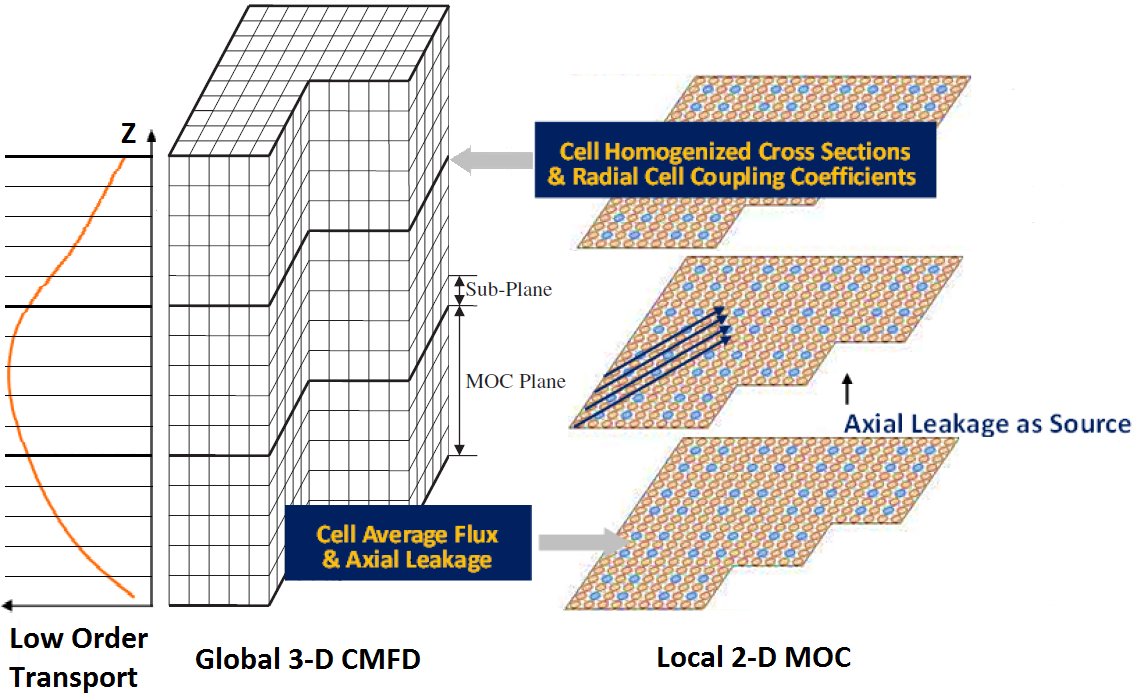
\includegraphics[width=0.8\textwidth]{../figs/2d1d-subplane.png}
    \caption[2D/1D Illustration]{The 2D/1D Method illustrated with the sub-plane scheme for the axial and CMFD calculations}
    \label{f:2d1dsubpalne}
\end{figure}

The second group of researchers was at Korea Atomic Energy Research Institute (KAERI).  They developed what is known more simply as the ``2D/1D'' scheme, first implemented in the DeCART code \cite{3DHetWholeCoreTransPlanarMOC,DeCARTTheoryManual,MethodsAndPerformanceOfDecart}.  This employs very similar technique to the 2D/1D Fusion method described above.  However, rather than using angular fluxes from each solver as a source term, currents are tallied on each of the six faces of each pin cell.  The currents can then be used to compute axial and radial ``transverse leakage'' sources for the radial and axial solvers, respectively.  This change allows for the storage of group-wise currents at each interface instead of storing the group-wise angular fluxes for each angle, significantly reducing the memory burden of the calculation.

After some development, the DeCART code was forked into several different versions for different institutions, one of them being the University of Michigan (UM).  After some development, it was determined that there would be no further development of the DeCART code at UM and a new 2D/1D implementation would be put in MPACT \cite{2D1DApproxTo3DTransport1,StabilityAndAccuracyOf3DTransportInMPACT}.  In MPACT's implementation of 2D/1D, 2D MOC is used for each of the radial planes, as with earlier 2D/1D codes.  The axial calculation done on a pin-homogenized mesh usually with SP$_3$, though a variety of other solver are available such as NEM, SENM, SP$_1$, SP$_5$, or S$_N$.  Finally, MPACT also uses 3D CMFD on the same pin-homogenized mesh to provide convergence acceleration to the calculations.  The remainder of this chapter will look at the derivation of the 2D/1D equations, the details of how they are implemented in MPACT, and some of the approximations and sources of errors related to this method.

\section{Derivation}

\subsection{Radial Equations}\label{ss:2d1dradialEq}

To derive the radial equations, we begin with the multigroup approximation in equation \ref{e:multigroupboltzmann}  and integrate in the $z$-direction over some range $\Delta z_i = z_{k+\frac{1}{2}} - z_{k-\frac{1}{2}}$.  To do this, we assume the cross-sections are all constant in the interval $z \in \left[z_{k-\frac{1}{2}},z_{k+\frac{1}{2}}\right]$.  With this assumption, we obtain the following equation:
\begin{subequations}
\begin{dmath}\label{e:2D1DradialEq}
{\Omega_x\frac{\partial \psi_{g}^Z}{\partial x} + \Omega_y\frac{\partial \psi_{g}^Z}{\partial y} + \frac{\Omega_z}{\Delta z_k}\left(\psi_{g,z_{k+\frac{1}{2}}} - \psi_{g,z_{k-\frac{1}{2}}}\right)} + {\Sigma_{t,g}\left(x,y\right)\psi_{g}^Z\left(x,y,\bm\Omega\right)} = {\frac{1}{4\pi}\sum_{g'=1}^{G}\intop_{4\pi}\Sigma_{s,g'\rightarrow g}^Z\left(x,y,\bm\Omega'\cdot\bm\Omega\right)\psi_{g'}^Z\left(x,y,\bm\Omega'\right)d\Omega'} + {\frac{1}{k_{eff}}\frac{\chi_{g}^Z}{4\pi}\sum_{g'=1}^G\intop_{4\pi} \nu\Sigma_{f,g'}^Z\left(x,y\right)\psi_{g'}^Z\left(x,y,\bm\Omega'\right)d\Omega'} + {\frac{Q_{g}^Z\left(x,y\right)}{4\pi}}
\end{dmath}
\begin{equation}
\psi_g^Z\left(x,y,\bm{\Omega}\right) = \frac{1}{\Delta z_k} \intop_{z_{k-\frac{1}{2}}}^{z_{k+\frac{1}{2}}} \psi_g^Z\left(x,y,z,\bm{\Omega}\right) dz
\end{equation}
\end{subequations}
where a superscript $Z$ indicates the average of a quantity over a given plane.  The $z$-component of the streaming can now be moved to the right-hand side of the equation and treated as a source term, giving a 2D transport problem which could be solved with a variety of methods:
\begin{subequations}
\begin{dmath}
{\Omega_x\frac{\partial \psi_{g}^Z}{\partial x} + \Omega_y\frac{\partial \psi_{g}^Z}{\partial y}} + {\Sigma_{t,g}\left(x,y\right)\psi_{g}^Z\left(x,y,\bm\Omega\right)} = {q_{g}^Z\left(x,y\right) + L_{g}^Z\left(x,y,\Omega_z\right)}
\end{dmath}
\begin{dmath}
q_{g}^Z\left(x,y\right) = {\frac{1}{4\pi}\sum_{g'=1}^{G}\intop_{4\pi}\Sigma_{s,g'\rightarrow g}^Z\left(x,y,\bm\Omega'\cdot\bm\Omega\right)\psi_{g'}^Z\left(x,y,\bm\Omega'\right)d\Omega'} + {\frac{1}{k_{eff}}\frac{\chi_{g}^Z}{4\pi}\sum_{g'=1}^G\intop_{4\pi} \nu\Sigma_{f,g'}^Z\left(x,y\right)\psi_{g'}^Z\left(x,y,\bm\Omega'\right)d\Omega'} + {\frac{Q_{g}^Z\left(x,y\right)}{4\pi}}
\end{dmath}
\begin{equation}
L_{g}^Z\left(x,y,\Omega_z\right) = \frac{\Omega_z}{\Delta z_k}\left(\psi_{g,z_{k-\frac{1}{2}}} - \psi_{g,z_{k+\frac{1}{2}}}\right)
\end{equation}
\end{subequations}
where $L_{g}^Z\left(x,y,\Omega_z\right)$ is the axial transverse leakage source term for plane $z$.  To simplify the source term, the axial transverse leakage term is often handled isotropically.  This is done by averaging over angle:
\begin{equation}
L_{g}^Z\left(x,y\right) = \frac{1}{4\pi}\intop L_{g}^Z\left(x,y,\Omega_z\right) \approx \frac{J_{g,z_{k-\frac{1}{2}}} - J_{g,z_{k+\frac{1}{2}}}}{4\pi\Delta z_k}
\end{equation}
where $J_{z_{i\pm \frac{1}{2}}}$ is the current at the top ($+$) or bottom ($-$) of the plane.  This eliminates the need for storing all the angluar fluxes on the top and bottom of every plane.  Other methods exist that allow the axial transverse leakage source to maintain its angular dependence without storing the angular fluxes \cite{KelleyBlakeThesis}, but these methods are not discussed here since they were not used by this work.

\subsection{Axial Equations}\label{ss:2d1daxialEq}

The axial equations can be derived in a manner similar to the radial equations.  Again, we begin with the multi-group approximation shown in equation \ref{e:multigroupboltzmann}.  This time, we integrate in both the x and y directions over intervals $x \in \left[x_{i-\frac{1}{2}},x_{i+\frac{1}{2}}\right]$ and $y \in \left[y_{j-\frac{1}{2}},y_{j+\frac{1}{2}}\right]$, giving the following equations in the axial direction, which are analogous to the radial equations in the previous section:
\begin{subequations}\label{e:2D1DaxialEq}
\begin{dmath}
{\Omega_z \frac{\partial \psi_{g}^{XY}}{\partial z}} + {\Sigma_{t,g}^{XY}\left(z\right)\psi_{g}^{XY}\left(z,\bm\Omega\right)} = q_{g}^{XY}\left(z,\Omega_x,\Omega_y\right) + {L_{g}^{XY}\left(z,\Omega_x,\Omega_y\right)}
\end{dmath}
\begin{dmath}
q_{g}^{XY}\left(z,\Omega_x,\Omega_y\right) = {\frac{1}{4\pi}\sum_{g'=1}^G\intop_{4\pi} \Sigma_{s,g'\rightarrow g}^{XY}\left(z,\bm\Omega'\cdot\bm\Omega\right)\psi_{g'}^{XY}\left(z,\bm\Omega'\right)d\Omega'} + {\frac{1}{k_{eff}}\frac{\chi_{g}^{XY}}{4\pi}\sum_{g'=1}^G\intop_{4\pi}\nu\Sigma_{f,g'}^{XY}\left(z\right)\psi_{g'}^{XY}\left(z,\bm\Omega'\right)d\Omega'} + {\frac{Q_{g}^{XY}\left(z\right)}{4\pi}}
\end{dmath}
\begin{dmath}
L_{g}^{XY}\left(z,\Omega_x,\Omega_y\right) = {\frac{\Omega_x}{\Delta y_i}\intop_{y_{i-\frac{1}{2}}}^{y_{i+\frac{1}{2}}} \left(\psi_{g,x_{i-\frac{1}{2}}}\left(y\right) - \psi_{g,x_{i+\frac{1}{2}}}\left(y\right) dy\right)} + {\frac{\Omega_y}{\Delta x_i}\intop_{x_{i-\frac{1}{2}}}^{x_{i+\frac{1}{2}}} \left(\psi_{g,y_{i-\frac{1}{2}}}\left(x\right) - \psi_{g,y_{i+\frac{1}{2}}}\left(x\right) dx\right)}
\end{dmath}
\begin{equation}\label{e:2D1DaxFluxDef}
\psi_g^{XY} = \frac{1}{\Delta_i \Delta_j} \intop_{y_{j-\frac{1}{2}}}^{y_{j+\frac{1}{2}}} \intop_{x_{i-\frac{1}{2}}}^{x_{i+\frac{1}{2}}} \psi_g\left(x,y,z,\bm{\Omega}\right) dx dy
\end{equation}
\end{subequations}
where a superscript $XY$ now corresponds to a particular x- and y-region which extends the full height of the problem in the z-direction.  Again, it is assumed that the cross-sections are constant in the x- and y-directions inside the region of integration.  How this is accomplished will be discussed in more detail when discussing MPACT's implementation of SP$_3$ and CMFD.

As with the radial equations, we can treat the transverse leakage source isotropically by averaging over angle:

\begin{dmath}
{L_{g}^{XY}\left(z\right)} = {\frac{1}{4\pi}\intop_{4\pi} L_{g}^{XY}\left(z,\Omega_x,\Omega_y\right)} \approx {\frac{1}{4\pi\\Delta y_i}\intop_{y_{i-\frac{1}{2}}}^{y_{i+\frac{1}{2}}}\left( J_{g,x_{i-\frac{1}{2}},y_i}\left(z\right) - J_{g,x_{i+\frac{1}{2}},y_i}\left(z\right)\right)dy} + {\frac{1}{4\pi\Delta x_i}\intop_{x_{i-\frac{1}{2}}}^{x_{i+\frac{1}{2}}}\left( J_{g,x_i,y_{i-\frac{1}{2}}}\left(z\right) - J_{g,x_i,y_{i+\frac{1}{2}}}\left(z\right)\right)dx}
\end{dmath}

Again, methods have been developed to angle the angle-dependence of the radial transverse leakage source \cite{StimpsonShaneThesis}, but this work used only isotropic radial leakage.

\section{Implementation}

\begin{figure}[h]
  \centering
  \begin{tikzpicture}[node distance=2cm]

% Begin
\node (start) [startstop] {Start};
\node (init) [io, right of=start, xshift=2.0cm] {Input, Initialize Solution};

% CMFD
\node (CMFD) [process, below of=init] {CMFD Eigenvalue Calculation};

% Nodal
\node (Nodal) [process, below of=CMFD] {Axial P$_3$ Calculation};

% MOC
\node (MOC) [process, below of=Nodal] {2D MOC Sweeps};

% Finish
\node (convCheck) [decision, below of=MOC, yshift=-1.5cm] {Fission Source, k-eff Converged?};
\node (out) [io, below of=convCheck,yshift=-1.5cm] {Output};
\node (stop) [startstop, right of=out, xshift=2.0cm] {Stop};

% Basic Arrows
\draw [arrow] (start) -- (init);
\draw [arrow] (init) -- (CMFD);
\draw [arrow] (CMFD) -- (Nodal);
\draw [arrow] (Nodal) -- (MOC);
\draw [arrow] (MOC) -- (convCheck);
\draw [arrow] (out) -- (stop);

% Fancy Arrows
\draw [arrow] (convCheck) -- node[anchor=west] {yes} (out);
\draw [arrow] (convCheck) -| node[anchor=north] {no} ([xshift=1.5cm]Nodal.east) |- (CMFD);

\end{tikzpicture}
  \caption{Calculation flow for 2D/1D scheme}\label{f:2d1d-flowchart}
\end{figure}

Now that the general 2D/1D scheme has been described, some attention should be given to the details of its implementation in MPACT.  Figure \ref{f:2d1d-flowchart} shows the calculation flow used by MPACT.  The first step is to perform a global 3D CMFD calculation to obtain pin-averaged flux and interface currents between each cell.  Next, the axial solver uses the radial currents calculated by CMFD as a radial transverse leakage source to obtain an axial transverse leakage source for the radial solver.  Finally, 2D MOC is used as the radial solver to obtain a solution with sub-pin resolution in each plane.

\subsection{3D Sub-plane CMFD}\label{ss:2d1d-3dcmfd}

The CMFD method was originally implemented in MPACT just as described in section \ref{ss:CMFD}.  To do this, each pin cell is homogenized using the quantities defined in equation \ref{e:CMFDhomogTerms} in every plane in the model.  The radial coupling coefficients defined in equation \ref{e:CMFDcouplingCoeffs} are obtained by calculating the current at the interface between each pair of pin cells using the 2D MOC sweeper, while the axial coupling coefficients are obtained from the axial currents calculated by the axial solve during the previous iteration.  The matrix for the 3D multi-group system can then be set up and solved, typically using the generalized Davidson eigenvalue solver.

In addition to this traditional 3D CMFD, MPACT also has the capability to use the sub-plane scheme.  This scheme was first developed by Cho et al. for the DeCART code \cite{DeCARTsubplane}.  Thin MOC planes are capable of causing instability in the 2D/1D scheme, but are sometimes required to maintain accuracy.  The sub-plane scheme allows users to increase the thickness of the 2D planes while still maintaining the accuracy of a fine axial mesh.  Later, the developers of the nTRACER code \cite{RyuBEAVRSnTRACER2015} also used the sub-plane scheme.  In addition to how it was used in DeCART, nTRACER also uses the sub-plane scheme as part of its rod decusping methods \cite{ICAPPcontrolRodDecuspingNTRACER}.  MPACT also uses sub-plane as part of a decusping treatment, which will be discussed in greater detail in chapter \ref{chap:cusping}.  This section will deal only with the basics of the sub-plane method as it was used in DeCART.


\subsubsection{Homogenization}

The difference between the sub-plane scheme and traditional CMFD is that the CMFD system is that the CMFD system is allowed to have multiple axial planes for each of the 2D planes in which the transport calculations are done.  This allows CMFD to capture sub-plane axial flux shapes that would otherwise be ignored.  To do this, a sub-plane scaling factor is introduced which will be used to provide an axial shape within a 2D plane:

\begin{align}
c_{g,i}^k &= \frac{\phi_{g,i}^{k-1}}{\overline{\phi}_{g,i}^{k-1}} \nonumber\\
 &= \frac{\phi_{g,i}^{k-1} \sum_{i'=1}^{N_{sp}} V_{i'}}{\sum_{i'=1}^{N_{sp}} \phi_{g,i'}^{k-1} V_{i'}}
\end{align}

where superscripts indicate which iteration the values are taken from and $N_{sp}$ is the number of sub-planes for the pin cell of interest.  Now when the homogenized values are calculated from the 2D transport solution using equation \ref{e:CMFDhomogTerms}, the fine mesh flux is multiplied by this sub-plane scaling factor everywhere it appears.  Because the 2D/1D scheme assumes a constant material axially in each plane, this sub-plane factor has no impact on the homogenized cross-sections.  However, the homogenized flux $\phi_{g,i}$ and fission source distribution $\chi_{g,i}$ will be changed, providing an axial shape for the source term in the eigenvalue calculation.

\subsubsection{Coupling Coefficients}

In addition to the homogenized cell terms, the coupling coefficients described by equations \ref{e:CMFDinterface} and \ref{e:CMFDcouplingCoeffs} must be calculated for each sub-plane.  To maintain consistency, the area-averaged current calculated by the radial sweeper must be preserved across the sub-surfaces used by the sub-plane scheme.  Thus, the current calculated by the radial sweeper at an interface is used at the corresponding interfaces for all sub-planes in that plane.  Additionally, to maintain consistency, this requires that the cell-homogenized flux used in the calculation of the diffusion coefficients be defined for the entire MOC plane as in equation \ref{e:CMFDhomogFlux} rather than using the sub-plane scaling factor for each sub-plane.

The axial coupling coefficient can be treated in a more straightforward manner.  Because the 1D axial solvers use the same pin-homogenized mesh as the CMFD solver, axial currents are naturally calculated at the top and bottom of each of the sub-planes.  Thus, these currents can be used together with the sub-planes fluxes to calculate sub-plane--dependent axial coupling coefficients.

\subsubsection{Projection}

The projection of the CMFD flux back to the 2D planes must also account for the presence of the sub-planes.  To do this, the solution is volume-averaged over all sub-planes for each pin cell, resulting in an equation similar to \ref{e:CMFDscaling}:

\begin{equation}
\phi_{trans,g,j}^k = \frac{\sum_{i'=1}^{N_{sp}} \phi_{CMFD,g,i'}^k V_i}{\sum_{i'=1}^{N_{sp}} \phi_{CMFD,g,i'}^k V_i} \phi_{trans,g,j}^{k-1}
\end{equation}

The calculation flow for 3D CMFD is shown in figure \ref{f:CMFD-flowchart}.

\begin{figure}[h]
  \centering
  \begin{tikzpicture}[node distance=2cm]

% Start
\node (start) [startstop] {Start};

% CMFD
\node (homog) [process, right of=start, xshift=2.0cm] {Homogenize Cross-sections and Flux; Calculate $\tilde{D}$};
\node (iterCheck) [decision, below of=homog, yshift=-1.5cm] {First Iteration?};
\node (firstIter) [process, below of=iterCheck, xshift=-2.5cm, yshift=-1.0cm] {Set $\hat{D}=0$};
\node (laterIter) [process, below of=iterCheck, xshift=2.5cm, yshift=-1.0cm] {Calculate $\hat{D}$};
\node (matrix) [process, below of=firstIter, xshift=2.5cm] {Set up CMFD Matrix};
\node (3DCMFD) [process, below of=matrix] {3D CMFD Calculation};
\node (proj) [process, below of=3DCMFD] {Scale MOC flux with CMFD flux};

% Stop
\node (stop) [startstop, right of=proj, xshift=2.0cm] {Stop};

% Basic Arrows
\draw [arrow] (start) -- (homog);
\draw [arrow] (homog) -- (iterCheck);
\draw [arrow] (matrix) -- (3DCMFD);
\draw [arrow] (3DCMFD) -- (proj);
\draw [arrow] (proj) -- (stop);

% Fancy Arrows
\draw [arrow] (iterCheck) -| node[anchor=south] {yes} (firstIter);
\draw [arrow] (iterCheck) -| node[anchor=south] {no} (laterIter);
\draw [arrow] (firstIter) |- (matrix);
\draw [arrow] (laterIter) |- (matrix);

\end{tikzpicture}
  \caption{Calculation flow for 3D sub-plane CMFD}\label{f:CMFD-flowchart}
\end{figure}

\subsection{1D SP\textsubscript{3}}

In MPACT, the 1D axial solvers operate on the same mesh as the 3D CMFD calculations, meaning that cell-homogenized quantities and radial currents have already been obtained from the CMFD calculation.  All the 1D axial solver must do is construct a source term from the radial currents for each cell, then perform a calculation to obtain currents on the axial interfaces at the top and bottom of each node.

MPACT has a variety of 1D nodal methods that are capable of performing these calculations, including diffusion-based such as NEM and SENM and higher-order solvers such as SP$_N$ and S$_N$.  For most MPACT calculations, including those in this work, the solver of choice is SP$_3$, which provides significant improvement over the diffusion-based methods and SP$_1$.  Very little benefit is obtained by using the higher-order SP$_5$.

\begin{figure}[h]
  \centering
  \begin{tikzpicture}[node distance=2cm]

% Begin
\node (start) [startstop] {Start};

% Nodal
\node (radialTL) [process, right of=start, xshift=2.5cm] {Calculate radial transverse leakage source};
\node (sp3-0) [process, below of=radialTL] {Solve 0th moment equation};
\node (sp3-2) [process, below of=sp3-0] {Solve 2nd moment equation};
\node (convCheck) [decision, below of=sp3-2, yshift=-1.5cm] {Converged?};

% Stop
\node (stop) [startstop, right of=convCheck, xshift=2.5cm] {Stop};

% Basic Arrows
\draw [arrow] (start) -- (radialTL);
\draw [arrow] (radialTL) -- (sp3-0);
\draw [arrow] (sp3-0) -- (sp3-2);
\draw [arrow] (sp3-2) -- (convCheck);
\draw [arrow] (convCheck) -- node[anchor=north] {yes} (stop);

% Fancy Arrows
\draw [arrow] (convCheck) -| node[anchor=north] {no} ([xshift=-1.5cm]sp3-2.west) |- (sp3-0);

\end{tikzpicture}
  \caption{Calculation flow for 1D axial calculations in MPACT}\label{f:Axial-flowchart}
\end{figure}

The SP$_3$ equations consist of equations for angular flux moments 0 through 3.  These equations can be combined into two equations for just the 0th and 2nd moments.  With the equations formulated this way, MPACT can iterate between the two moments until they converge, then calculate axial currents and move on to the radial calculations.

While SP$_3$ handles the angle dependence of the flux, it does not handle the spatial dependence.  To do this, the SP$_3$ solvers are wrapped in a two-node NEM solver.  This method assumes that the flux has a fourth-order polynomial shape in space and that the source term has a second-order shape.  Using the neighboring cells above and below each cell, this source term shape is constructed and used to solve for the 0th moment of the flux.

\subsection{2D MOC}

For the radial calculations, 2D MOC is used.  This allows MPACT to easily calculate scalar fluxes and currents in each plane regardless of the geometric complexity.  This section is devoted to discussing some of the details of the MOC implementation and sweeping algorithm in MPACT.

\subsubsection{Ray Tracing}

\begin{figure}[h]
    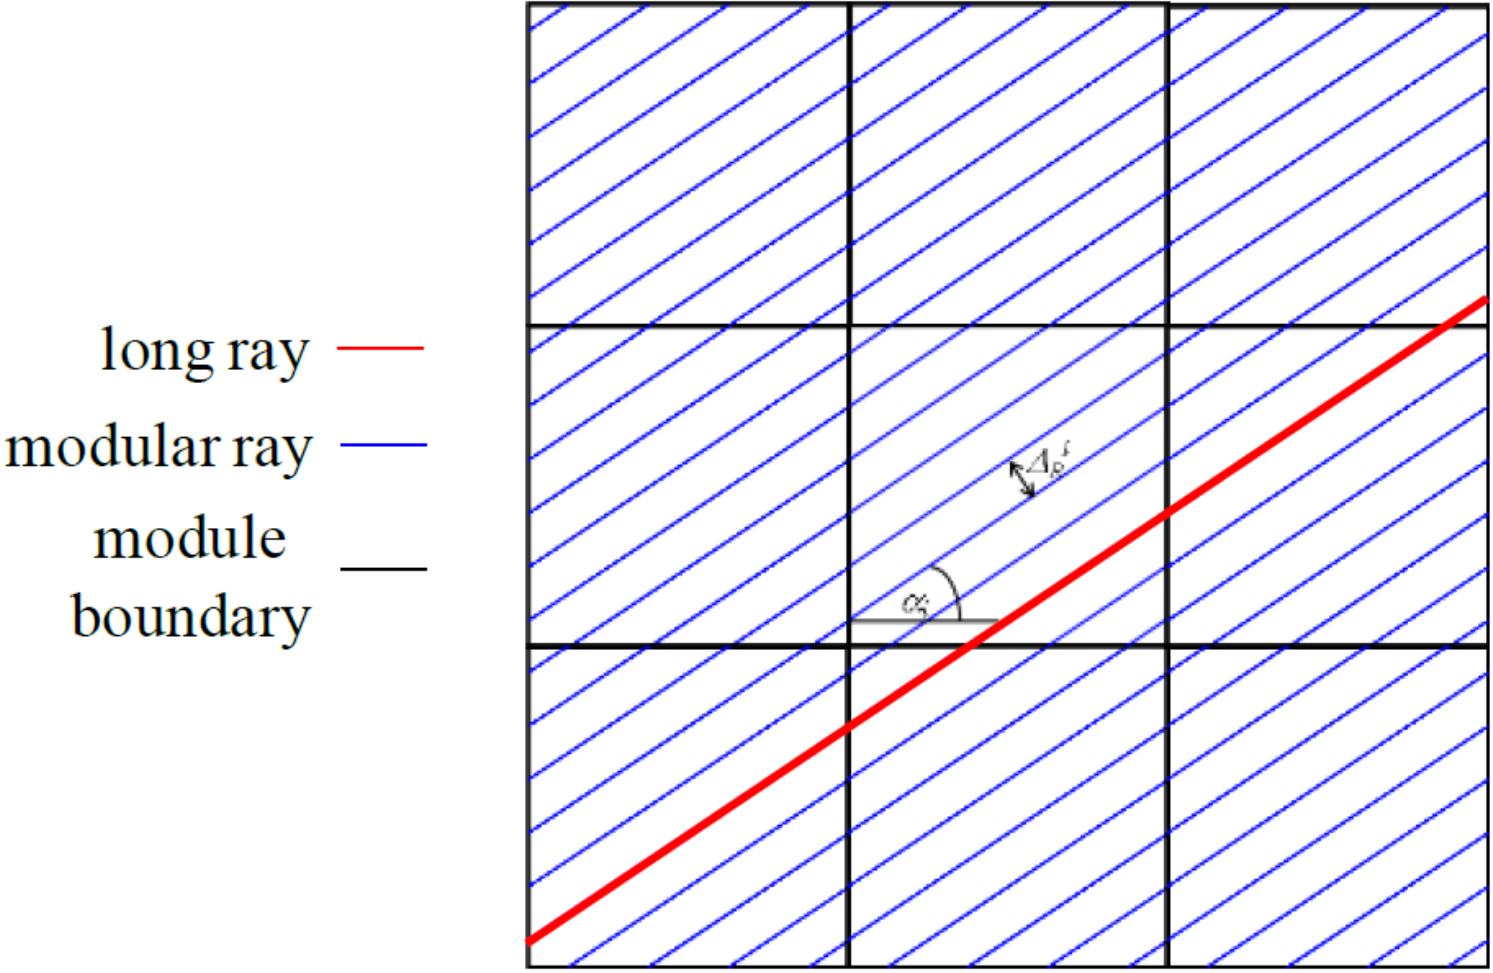
\includegraphics[width=0.5\textwidth]{modular_rays.png}
    \caption[Modular Ray Tracing]{Modular ray tracing depiction \cite{MPACTTheoryManual}}\label{e:ModRays}
\end{figure}

One of the key features of MPACT's MOC implementation is that of modular ray tracing.  Ray tracing is performed once at the beginning of a calculation and stored for the remainder of the calculation.  Doing this greatly reduces the runtime of the MOC sweeps since the length of each ray segment and the region it is crossing are already known ahead of time.  Furthermore, MPACT takes advantage of the repeatable nature of a reactor's geometry.  Because reactor geometry is repetitive, small portions of the geometry which repeat frequently can be ray-traced separately instead of tracing the entire core.  These smaller units of geometry are known as ray tracing modules, and in MPACT can be a full fuel assembly, a quarter fuel assembly, or a single fuel pin.  After the unique modules are identified, each of them is ray-traced in such a way that the endpoints of a ray in each module will line up with the beginning of a ray in the neighboring module.  This significantly reduces the storage requirements for the ray data since a small number of ray tracing modules can represent a full core problem.

As a result of the modular ray tracing, several corrections are required.  First, to successfully perform the ray tracing the angles of the rays had to be adjusted slightly to line up.  However, because a quadrature is used to integrate the angular flux, this angle modification requires a correction to the quadrature weights as well to maintain accuracy.  Second, the spacing between the rays must also be adjusted slightly to ensure that all rays align.  Along with these corrections, there are other MOC concepts such as volume corrections, cyclic rays, and others which are important to be aware of but will be deferred to the MPACT theory manual for details \cite{MPACTTheoryManual}.

\subsubsection{Sweeping Algorithm}\label{sss:2d1dMOCsweepAlgorithm}

\begin{figure}[h]
  \centering
  \begin{tikzpicture}[node distance=2cm]

% Begin
\node (start) [startstop] {Start};
\node (init) [io, right of=start, xshift=2.5cm] {Input N$_{inners}$};

% MOC
\node (begin) [process, below of=init] {Set $n=0$};
\node (source) [process, below of=begin] {Calculate fission and axial transverse leakage sources};
\node (scatSource) [process, below of=source] {Calculate scattering source};
\node (MOC) [process, below of=scatSource] {2D MOC sweep over each energy group};
\node (MOCdone) [decision, below of=MOC, yshift=-1.5cm] {$n = N_{inners}$?};z
\node (stop) [startstop, right of=MOCdone, xshift=2.5cm] {Stop};

% Basic Arrows
\draw [arrow] (start) -- (init);
\draw [arrow] (init) -- (begin);
\draw [arrow] (begin) -- (source);
\draw [arrow] (source) -- (scatSource);
\draw [arrow] (scatSource) -- (MOC);
\draw [arrow] (MOC) -- (MOCdone);

% Fancy Arrows
\draw [arrow] (MOCdone) -| node[anchor=north] {no} ([xshift=-1.5cm]MOC.west) |- (scatSource);
\draw [arrow] (MOCdone) -- node[anchor=north] {yes} (stop);

\end{tikzpicture}
  \caption{Calculation flow for 2D MOC calculation in MPACT}\label{f:MOC-flowchart}
\end{figure}

To perform the MOC sweeps, MPACT uses a multi-group sweeping method.  To do this, multi-group sources and cross-sections are prepared for each of the fine mesh regions in each plane.  There are then four total loops for the sweeping algorithm.  From outermost to innermost, these loops are over azimuthal angle, ray (across the entire domain), polar angle, and energy group.  Each ray is divided into many segments that the MOC steps its way along as described in section \ref{ss:MOCtheory}.  As these sweeps are performed, scalar flux is tallied in each fine mesh region, and, assuming CMFD is being used, currents are tallied at the interfaces between each pin cell.  Normally only one inner MOC iteration is required per 2D/1D iteration.  This algorithm is shown in figure \ref{f:MOC-flowchart}.

MPACT also has the capability of performing the MOC sweeps with the energy loop as the outermost.  This has two advantages.  First, the previous group is used to construct the scattering source for the current group.  This means that the iteration scheme is a Gauss-Seidel iteration instead of a Jacobi iteration, which can speed up the convergence of the problem.  Secondly, the cross-sections and sources only need to be stored for one group at a time, minimizing the storage requirements for the calculations.  However, when using transport-corrected cross-sections, some instabilities have been observed in this iteration scheme when using only a single inner iteration.  Further more, having the energy loop on the inside results in some improved cache efficiency when it comes to traversing the rays, reducing the runtime for a single MOC sweep \cite{JacobiInscatterTechReport}.  For these two reasons, MPACT defaults to the Jacobi-style iteration scheme described first.

\section{Parallel Decomposition}

While the 2D/1D scheme greatly reduces runtime from a direct 3D transport calculation, it is still computationally expensive when compared to nodal methods traditionally used by industry.  To minimize the walltime required for 2D/1D calculations in MPACT, several different methods of decomposing the problem for parallel execution have been implemented.  These methods allow MPACT to easily scale to hundreds or thousands of CPUs.  Each of these methods will be briefly described in this section.

\begin{enumerate}[leftmargin=*]
\item \textbf{Spatial Decomposition}

When using this decomposition, each parallel process only has a portion of the model.  Each portion is solved locally by one process, then boundary data is communicated to all processes which own neighboring portions of the model.  The updated boundary data is then used in the following iteration.  When using spatial decomposition, planar decomposition is performed first.  This means that if the total number of parallel processes being used is less than or equal to the number of 2D MOC planes, then one or more entire planes is simulated by each process.  If more processes are used than there are planes in the model, then radial decomposition is performed.  This decomposes every plane radially into smaller pieces.  Every plane must be radially decomposed in the same way, and the smallest unit allowed in radial decomposition is a single ray-tracing module.  Because spatial decomposition does not duplicate much memory and does not decrease the computational efficiency significantly, it is usually the preferred choice of decomposition methods.

\item \textbf{Angle Decomposition}

For angle decomposition, each process has the entire spatial domain.  When the MOC sweeps are performed, each process only sweeps a subset of the angles in the selected quadrature.  After the sweep, a reduction is performed to get the actual scalar flux and currents on all processes.  For the CMFD calculation, the angle processes are re-purposed as spatial processes.  Each angle process owns the full domain, but only solves a portion of it as if it were spatially decomposed.

It is possible to use both spatial and angle decomposition together.  When this is done, spatial decomposition is performed first, then angle decomposition is done within each spatial domain.  In general, the efficiency of angle decomposition calculations is less than that of spatial decompositions.  Furthermore, it also requires that each angle process models all of the spatial domain, increasing the total memory required for the calculation compared with finer spatial decomposition.  However, angle decomposition is still useful for reducing the runtime of cases where further spatial decomposition is not possible.

\item \textbf{Ray Decomposition}

A third type of decomposition that can be done is to decompose the rays in the MOC calculation.  Unlike the previous methods, the ray decomposition makes use of shared-memory threading instead of distributed memory message passing.  While performing the MOC sweeps, several threads are used to solve all the rays in each angle.  For the CMFD calculation, MPACT has internal RBSOR solvers which are capable of using threading.  However, when third-party libraries are used for the CMFD calculations, the threading will be used only during the CMFD calculation.  Threading can also be combined with both spatial and angle decomposition to further increase the parallelism of MPACT.

\item \textbf{Energy Decomposition}

At this time, energy decomposition is not available in MPACT.  However, when it is added, it will be similar to the angle decomposition.  For the MOC calculation, each process will solve a subset of the energy groups on the spatial domain, and for the CMFD calculation, the energy processes will be re-purposed as space processes.
\end{enumerate}

\section{Sources of Error}\label{s:2d1dErrors}

The 2D/1D approximation as several sources of error.  Some of these are addressed by mesh, ray spacing, or quadrature refinements, but others are due to approximations made in the method itself.  The sources of error which are due to fundamental approximations in the 2D/1D method will be discussed first, followed by a brief (not comprehensive) list of some other common sources of error.

\subsection{Axial Homogenization}

When deriving the radial equations in section \ref{ss:2d1dradialEq}, it was assumed that the cross-sections were constant in the axial direction for each of the planes.  While this is often the case if an appropriate axial mesh is selected, sometimes it is impractical to mesh the problem finely enough to ensure this.  When an axial material heterogeneity is present in a plane, 2D MOC requires that these materials be homogenized.  In some cases, a simple volume-averaging is sufficient, but if a material with a large cross-section is being homogenized with a material that has a significantly different cross-section, significant errors can result.  To prevent this without refining the axial mesh, some modification to the 2D/1D scheme is required to improve the homogenization.  This will be addressed in chapter \ref{chap:cusping}.

\subsection{Axial Transverse Leakage Source}

Another approximation relates to the assumptions made while deriving the axial equations in section \ref{ss:2d1daxialEq}.  The SP$_3$ calculations are performed on a pin-homogenized mesh.  Because of this, the axial currents used in the axial TL source are assumed to be flat across the entire pin cell.  However, the currents will obviously be quite different in the fuel and moderator regions.  Furthermore, the axial TL is treated isotropically.  While this simplifies the axial calculations and MOC storage requirements, it does not perfectly reflect reality.  Both these spatial and angular assumptions introduce some error into the axial TL source used by MOC.

\subsection{Radial Currents}

The radial TL source used by the axial SP$_3$ solver has the same two approximations as the axial TL source did.  Radial currents are used to generate the source, which assumes isotropy.  Additionally, the spatial shape is flat across each pin cell.  This is corrected to some extent since the axial solver produces a quadratic source shape using the neighboring nodes, but this is not a perfect solution.

Additionally, when using the sub-plane method, the $\hat{D}$ correction terms used by CMFD are assumed to be axially flat within each MOC plane.  While this assumption improves the stability of the calculations, it forces CMFD to capture any axial shape the current has within an MOC plane.  For most problems, this error is probably negligible, but for cases such as a partially inserted rod or other strong absorber, it would be beneficial to be able to have sub-plane--dependent $\hat{D}$ terms to more accurately calculate the radial currents.  Doing this would improve the radial TL source in the SP$_3$ solver, and the the overall 2D/1D results.

\subsection{Other Sources of Error}

Several other sources of error in the 2D/1D method will be briefly mentioned here, but not discussed in detail.

\begin{enumerate}[leftmargin=*]
  \item \textbf{Ray Spacing}
  
  The spacing between the rays in the MOC calculation is important to the accuracy of the calculation.  At minimum, one ray needs to pass through each of the fine mesh regions, but multiple rays will improve the accuracy.  A typical ray spacing is 0.05 cm, but sometimes finer spacing may be required.
  
  \item \textbf{Radial Meshing}
  
  The radial and azimuthal meshing of each of the pin cells must be fine enough to give a good solution.  In MPACT, fuel pins usually have 3 radial rings, with an extra ring in the moderator region to resolve the change in the flux near the edge of the fuel pin.  Each ring is typically divided into 8 azimuthal regions.
  
  \item \textbf{Axial Meshing}
  
  The axial mesh must be refined enough to capture the axial shape of the solution.  Usually MOC planes of about 8 cm thick are used for a typical PWR calculation, which some thinner planes to resolve spacer grids, burnable poison inserts, or other components.  Using thicker planes could decrease accuracy and worsen the convergence of the calculation.
  
  \item \textbf{Scattering Treatment}
  
  Scattering in a reactor, especially off the hydrogen atoms in the moderator, is anisotropic.  To resolve this, a sufficiently high-order scattering treatment must be used in the MOC calculations.  For PWRs, $P_1$ to $P_3$ is a typical range.  MPACT is capable of going up to P$_5$ scattering treatment for libraries which have the required data.
  
  An alternative is to use transport-correction P$_0$ scattering.  This can capture the anisotropy without increasing the runtime of the calculations.  However, there are several methods of calculating the transport cross-sections, and none of them are perfect.  Thus, using the TCP$_0$ option in MPACT also has some non-trivial error associated with it.
  
  \item \textbf{Cross-Section Library}
  
  To perform any calculations using the 2D/1D method, a multi-group cross-section library must be available.  While this is not technically a source of error in the 2D/1D method itself, the cross-section library can be difficult to generate correctly.  Any error in any isotope in the library will cause error in the 2D/1D calculations if the isotope is used in the model.  Thus, the 2D/1D method is useless if the a bad cross-section library is being used.
  
  \item \textbf{Self-Shielding}
  
  Another potential source of error is related to spatial and energy self-shielding.  To correctly deal with resonance absorption in the fuel while also accounting for the spatial self-shielding in the fuel, MPACT uses the subgroup method \cite{SubgroupOrig1974,SelfShieldingMethodologyMPACT2013}.  Without using this method, the k$_{eff}$ calculated by MPACT is off by several percent, along with an inaccurate flux distribution.
  
  \item \textbf{Quadrature}
  
  One final source of error that can arise is in the selection of a quadrature.  It is important to select both an appropriate number of azimuthal and polar angles as well as an appropriate type of quadrature.  Typically around 16 azimuthal angles and 3 polar angles is sufficient.  There are several different types of quadratures implemented in MPACT, but generally a Tabuchi-Yamamoto quadrature is used for the polar angles \cite{YamamotoQuadrature2012} with a Chebyshev quadrature for the azimuthal angles \cite{HandbookOfMathFunctions1972}.
\end{enumerate}

\section{Rod Cusping}
This chapter will focus specifically on control rod cusping effects, which are the focus of this work.  First, a more thorough definition of the problem and motivation for solving it will be presented.  The next section will then present some of the solutions that have been used to minimize the cusping effects in the past, including a simplified decusping model implemented in MPACT itself.  The third section will then discuss some newer methods based on the sublpane CMFD scheme that have recently been implemented in MPACT.  Finally, a new ``sub-ray'' MOC method will be proposed to deal with the cause of the cusping effects on a more fundamental level.

\section{Background}

In Section \todo{section num}, some potential sources of errors for the 2D/1D scheme were introduced.  One of these was the error introduced by axial homogenization within a 2D MOC plane.  In some cases, this can be done without introducing significant errors.  For example, MPACT often homogenizes components outside the active fuel region, such as the end plugs and gaps at the end of the fuel rods.  However, when strong neutron absorbers, such as control rods, are homogenized axially in active fuel region, this has the effect of introducing absorption in regions where there should be none.  This effect is known as ``cusping,'' and is illustrated in Figure 

\begin{figure}
    \centering
    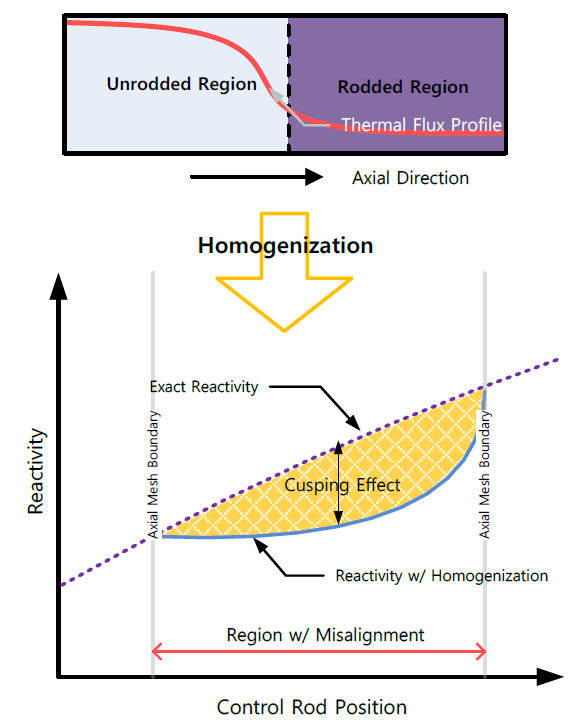
\includegraphics[width=0.4\textwidth]{cusping_effect_Joo.png}
    \caption{Illustration of Rod ``Cusping''}\label{f:cuspingEffectJoo}
\end{figure}
\todo{cite}

In some cases, this is easily handled by setting up an appropriate axial mesh which prevents the need for the homogenization, but this is not always a practical solution.  Throughout the course of an entire cycle of operation (usually about 18 months), several different control banks in the reactor may move to a variety of positions to maintain criticality in the core.  Control rods in a PWR typically have step sizes of approximately 1.5 cm, but a typical MOC plane in MPACT is about 8 cm thick in the active fuel region.  In order to prevent cusping effects for an entire cycle, the user may have to create a very detailed axial mesh to ensure that all the control rod positions used throughout the cycle align with the edge of an MOC plane.  Not only is this tedious for the user, but it also greatly increases the computational burden due to the increased number of MOC planes.  Figure \ref{f:p4cuspingEffects} shows the calculated k-eff as a function of control rod position.  The cusping effects in this figure are further complicated by a heterogeneous rod with AIC and B$_4$C poison regions and a stainless steal tip.  Thus, cusping effects occur not just at the control rod tip, but also at material interfaces throughout the rod.

\begin{figure}
    \centering
    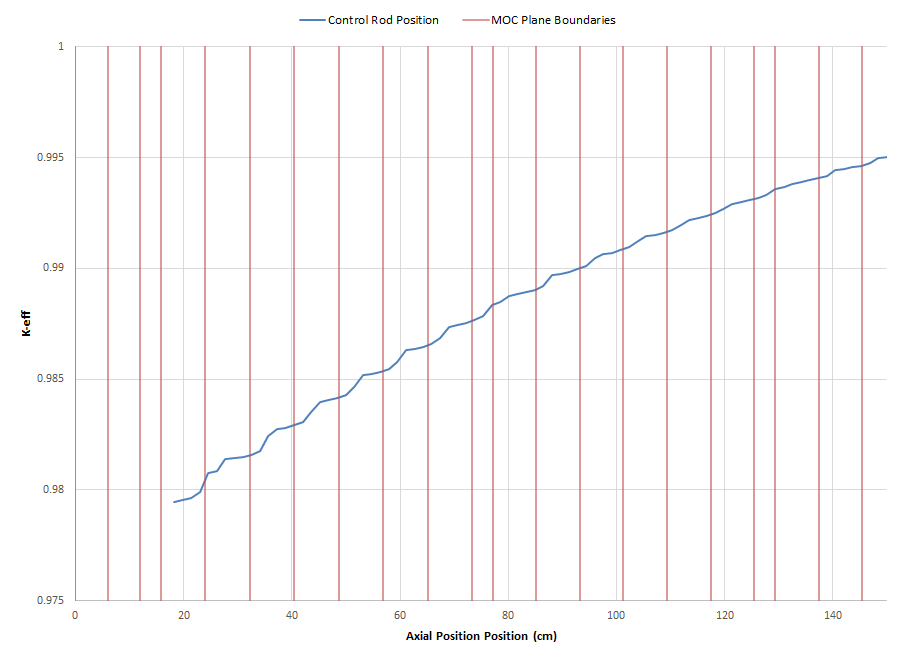
\includegraphics[width=0.8\textwidth]{p4cuspingEffects.png}
    \caption{Control Rod Cusping Effects for 3x3 Assembly}\label{f:p4cuspingEffects}
\end{figure}

\section{Traditional Solutions}

\subsection{Nodal Codes}

\todo{Legacy decusping methods}

\subsection{2D/1D Codes}\label{ss:2d1d-old-decusping-methods}

Several codes that have employed the 2D/1D method in recent years have also required rod decusping methods.  MPACT currently uses a simple polynomial correction to the volume fractions used to homogenize the control rod \cite{MC2015_VCS_Cycle_Depletion}.  To develop this method, a 3x3 assembly was set up with a control rod in the center assembly.  This problem was simulated with the rod tip at nine different positions in the plane.  These simulations were then repeated, but with the axial mesh refined so the rod tip aligned with a plane boundary.  The k-eff differences between the two sets of simulations were fitted with a sixth-order polynomial which is used in MPACT to reduce the volume fraction of the control rod by an appropriate amount to offset the cusping effects.  This process was repeated for different control rod materials such as AIC, B$_4$C, and Tungsten, since each material has unique cross-sections.  This method has the advantages of being simple to implement and requiring no increase in computational requirements.  However, the results obtained from this decusping method are tied to the control rod material and reactor model used to develop the corrections, limiting its usefulness to a small subset of reactors.

Another 2D/1D code is nTRACER, which is under active development by Seoul National University\todo{new citation}.  To address rod cusping effects in nTRACER, Jung and Joo developed a more general method than the polynomial correction method used by MPACT \cite{ICAPPcontrolRodDecuspingNTRACER}.  This method pre-generates correction factors at the start of a simulation, rather than relying on hard-coded corrections.  To do this, the assembly that will have a partially inserted control rod is identified, and a single-plane 3x3 assembly problem is set up using the partially-rodded assembly and its neighbors.  The radial and axial cusping effects are then determined separately.  First, the radial cusping effects are determined by performing 2D MOC calculations on the 3x3 sub-domain with the rod fully inserted and fully withdrawn.  This provides radial flux profiles in the rodded assembly for both rodded and unrodded regions, as well as current coupling coefficients for CMFD for the rodded and unrodded CMFD nodes.  Once this is done, the rod is simulated at positions of 25\%, 50\%, and 75\% withdrawn from the plane.  To reduce runtime, these calculations are done using only 3D sub-plane CMFD.  This generates axial flux profiles for the full MOC plane for each of the possible rod positions.  During the full-core 2D/1D calculation, these axial flux profiles are then used to generate improved homogenized cross-sections for the MOC calculation using equation.

\begin{equation}\label{e:nTRACERdecusping}
\overline{\Sigma_i} = \frac{\phi_{rad,i}^R \phi_{ax,i}^R \Sigma_i^R h^R + \phi_{rad,i}^U \phi_{ax,i}^U \Sigma_i^U h^U}{\phi_{rad,i}^R \phi_{ax,i}^R h^R + \phi_{rad,i}^U \phi_{ax,i}^U h^U}
\end{equation}

\todo{Look into other 2D/1D codes (decart)}

\section{Improved Decusping Methods}
\todo{Better Title?  Not that much ``better''}

This section discusses two new decusping treatments added to MPACT.  These methods rely on the sub-plane scheme described in section \todo{ref}.  The first method only treats the axial cusping effects, while the second method extends the first by also treating the radial decusping effects.

\subsection{Sub-plane Decusping}

In section \todo{section num}, the sub-plane scheme was introduced as a means of coarsening the 2D/1D axial mesh to improve runtime while maintaining accuracy.  However, one negative consequence of using the sub-plane scheme is that it increases the likelihood of partially inserted rods being present since there are fewer, thicker MOC planes.  To address this, two modifications were made to the sub-plane scheme to minimize cusping effects.

The first modification that was made was to modify the cross-sections used for the sub-plane CMFD and axial SP$_3$ calculations.  In the most basic form of the sub-plane scheme, the same cross-sections and radial coupling coefficients are used for all sub-planes in each MOC plane.  To use sub-plane as a decusping method, the requirement for constant cross-sections was removed.  Thus, when equation \ref{e:CMFDhomogTerms} is applied, explicit rodded or unrodded cross-sections are used for the cross-section homogenization in each sub-plane, rather than a single homogenized cross-section being using in all sub-planes.  This allows the CMFD and axial solvers to capture the sharp flux gradients that occur around the edge of the control rods.

In order to improve the MOC calculations as well, the CMFD flux projection described in equation \ref{e:CMFDscaling} is extended to also include a cross-section projection for the partially rodded pin cells.  This is done using equation \ref{e:nTRACERdecusping} with $\phi_{rad,i}^R = \phi_{rad,i}^U$.  This allows the 2D MOC calculations to also capture some of the axial effects of the partially inserted rod.

\subsection{Auxiliary 1D Collision Probabilities}

While the sub-plane decusping method is better than none, it captures only the axial effects of the partially inserted rod.  To also capture the radial effects, an additional radial calculation is needed to obtain radial flux profiles for the rodded and un-rodded regions.  In MPACT, this is done using a 1D Collision Probabilities (CP) solver.

After the CMFD homogenization, but prior to the calculation itself, a 1D CP kernel is solved for the rodded and un-rodded regions to obtain a radial flux profile.  These profiles are normalized so that the volume-average of each profile is exactly unity.  These profiles are then used with the sub-plane CMFD flux and material cross-sections to calculate improved homogenized cross-sections, as shown in equation \ref{e:CPMxs}.  Homogenizing the cross-sections in this way allows CMFD to capture both axial and radial effects of the partially inserted rod with negligible increase in computational expense.  This process is illustrated in figure \ref{f:CPdecusp}.

\begin{equation}\label{e:CPMxs}
\Sigma_{g,i}=\frac{1}{\phi_{g,i}V_i}\sum_{r=1}^{N_{rings}} \Sigma_{g,r} \phi_{CMFD,g,i} \phi_{CP,g,r} V_r
\end{equation}

\begin{figure}
  \centering
  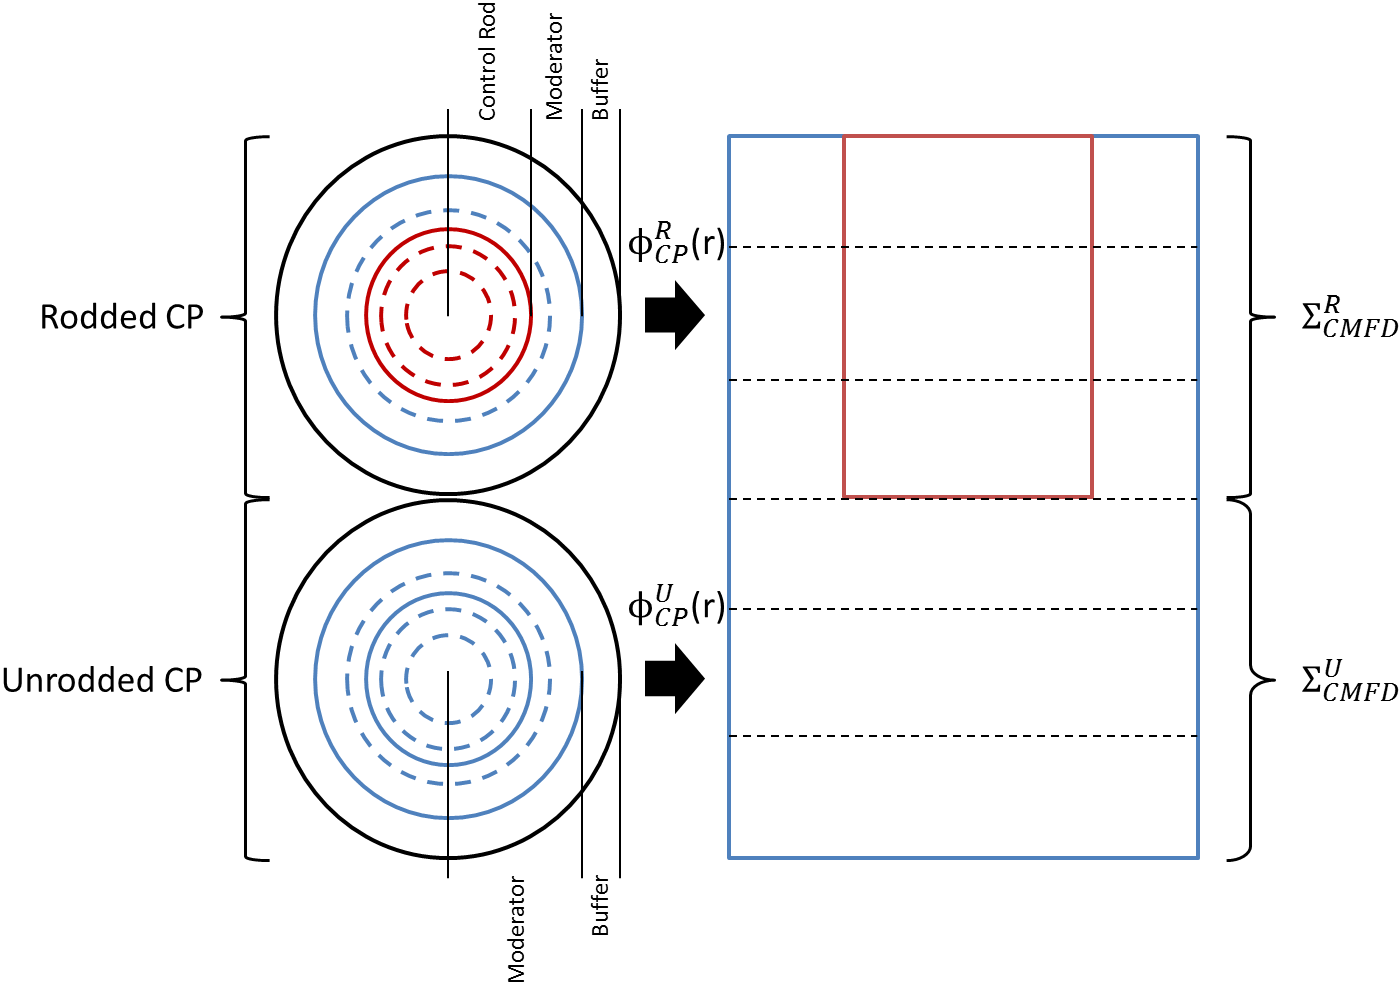
\includegraphics[width=\textwidth]{CPdecusp.png}
  \caption[Collision Probabilities Decusping]{Illustration of 1D Collision Probabilities rod decusping method}\label{f:CPdecusp}
\end{figure}

After the CMFD calculation, the MOC cross-sections must be modified as with the sub-plane decusping.  This is done using by using equation \ref{e:nTRACERdecusping} directly, where the radial flux terms are the projected MOC fluxes and the axial flux terms are the results of the sub-plane CMFD calculation that used the CP-homogenized cross-sections.  The projection of the CMFD flux to the MOC mesh is unchanged from the standard sub-plane scheme.  The CMFD calculation flow when using 1D CP is shown in figure \ref{f:1dcpm-flowchart}

\begin{figure}
  \centering
  \begin{tikzpicture}[node distance=2cm]

% Start
\node (start) [startstop] {Start};

% CMFD
\node (homog) [process, right of=start, xshift=2.0cm] {Homogenize cross-sections and flux; Calculate $\tilde{D}$};
\node (1dcpm) [process, below of=start, yshift=-0.5cm] {1D CP calculations};
\node (homogCP) [process, right of=1dcpm, xshift=2.0cm] {Re-homogenize cross-sections in partially rodded pin cells};
\node (iterCheck) [decision, below of=homogCP, yshift=-1.5cm] {First iteration?};
\node (firstIter) [process, below of=iterCheck, xshift=-2.5cm, yshift=-1.0cm] {Set $\hat{D}=0$};
\node (laterIter) [process, below of=iterCheck, xshift=2.5cm, yshift=-1.0cm] {Calculate $\hat{D}$};
\node (matrix) [process, below of=firstIter, xshift=2.5cm] {Set up CMFD matrix};
\node (3DCMFD) [process, below of=matrix] {3D CMFD calculation};
\node (proj) [process, below of=3DCMFD] {Scale MOC flux with CMFD flux};
\node (projCP) [process, below of=proj] {Homogenize partially rodded MOC cross-sections};

% Stop
\node (stop) [startstop, right of=projCP, xshift=2.0cm] {Stop};

% Basic Arrows
\draw [arrow] (start) -- (homog);
\draw [arrow] (1dcpm) -- (homogCP);
\draw [arrow] (homogCP) -- (iterCheck);
\draw [arrow] (matrix) -- (3DCMFD);
\draw [arrow] (3DCMFD) -- (proj);
\draw [arrow] (proj) -- (projCP);
\draw [arrow] (projCP) -- (stop);

% Fancy Arrows
\draw [arrow] (homog) |- ([yshift=-0.75cm]start.south) -| (1dcpm);
\draw [arrow] (iterCheck) -| node[anchor=south] {yes} (firstIter);
\draw [arrow] (iterCheck) -| node[anchor=south] {no} (laterIter);
\draw [arrow] (firstIter) |- (matrix);
\draw [arrow] (laterIter) |- (matrix);

\end{tikzpicture}
  \caption[Stuff]{Calculation flow for CMFD calculation in MPACT with 1D CP decusping treatment}\label{f:1dcpm-flowchart}
\end{figure}
\section{Polynomial Decusping}

\section{Subplane Collision Probabilities}

\subsection{Subplane CMFD}

\subsection{Collision Probabilities Decusping}

\section{Subray Method of Characteristics}

\subsection{Motivation}

\subsubsection{1D MOC Code and Problem Description}

The code is set up to take in a description of pins and materials to be used for the calculations.  For the geometry, a pin pitch is specified which is used for all pins.  Each pin consists of a list of radii.  Assuming a square pin cell, these pins are then transformed from cylindrical geometry to slab geometry while preserving the volume fraction of each material.  Thus, the thickness of the pin slab is equal to the pin pitch, but the width of the fuel material will not be equal to input radius, since the volume fractions are preserved.  One material is then specified for each region, though each material region is divided into many sub-regions for the MOC calculations.  These materials are defined by a separate cross-section library file.  This file uses the ``user library'' format supported by MPACT, which allows the user to put in macroscopic cross-sections for absorption, nu-fission, kappa-fission, chi, and scattering moments.  For all these calculations, the C5G7 benchmark cross-sections \cite{EELewisC5G72003,EELewisC5G7extended2005} were used.  These cross sections are included in Appendix \ref{app:c5g7xs}.

For the MOC sweeps, a Gaussian quadrature \cite{HandbookOfMathFunctions1972} is used with 2, 4, 8, 16, or 32 polar angles, with half of the angles being used in each direction.  The MOC sweeps are done similarly to how they are done in MPACT, with the loop over energy groups being the innermost loop.  The code can be run as either a fixed source solver or an eigenvalue solver.  For the eigenvalue mode, power iteration is used after each MOC calculation to determine and updated k$_{eff}$.  The fixed source mode can be used to run either a specified number of iterations or to run until the scattering source is converged below some tolerance.  This allows some flexibility on exactly what kinds of results can be obtained.

The problem used for these calculations was a 1D variation of VERA Problem 4.  The center row of pins across all three assemblies was pulled out and used for the 1D model, resulting in a row of 3$\times$17 pins with a pin pitch of 1.26 cm (the inter-assembly gap was neglected for this model).  The center assembly had 4 guide tubes in it which contained a mixture of moderator and control rod to represent a partially inserted control rod.  These partially rodded locations were the only part of the problem that had any material changes.  This allowed the effects of the cross-section homogenization to be isolated for each calculations.

\subsubsection{1D MOC Results}

\paragraph{Specified Total Source}

The first set of calculations performed were done using a specified total source.  To do this, the guide tubes were filled with 50\% control rod and 50\% moderator by volume fraction, and a full eigenvalue calculation was performed.  The source distribution from this calculation (both fission and scattering source) were then passed to the the fixed source solver.  A single iteration was run using this source on three different variations of the problem: the 50-50 mixture, fully rodded, and fully unrodded.  Because the multi-group source is set up before performing any MOC sweeps, this resulted in all three of those calculations having an identical source for the MOC sweep.  The only difference between them was the cross-sections used in the guide tubes.

Figure \ref{f:1dmoc-fixed-50-scalflux7} shows the scalar flux resulting from these three calculations.  The most important thing to note in this data is that the effects of the rod are very local in the MOC calculation.  Moving through the rodded pin cell, the rodded, unrodded, and mixed cases have converged back to the same shape by the time the edge of the pin cell is reached.  This indicates that whatever treatment is used for the partially rodded cell likely does not need to worry about interference between neighboring rods because the effects are so localized.

\begin{figure}[H]
    \centering
    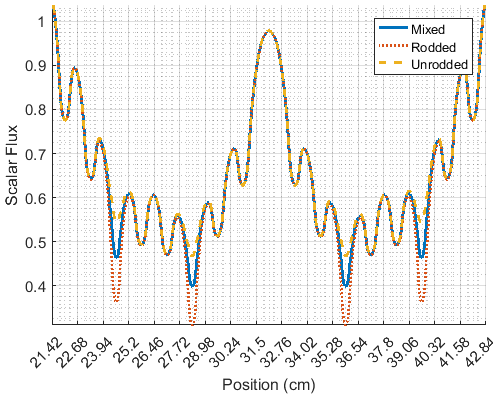
\includegraphics[width=0.7\textwidth]{1dmoc-50mix-fixedscat-scalflux7.png}
    \caption{Group 7 scalar flux comparisons for a fixed fission and scattering source calculation}\label{f:1dmoc-fixed-50-scalflux7}
\end{figure}

Figure \ref{f:1dmoc-fixed-50-angflux} shows the right-going angular flux in groups 1 (fast) and group 7 (thermal).  The group 7 angular flux behaves similarly to the group 7 scalar flux in that the effects are localized around each rod.  The three different angular flux shapes are still somewhat different at the edge of the neighboring pin cell, but have pretty much converged upon reaching the clad and fuel.  The reason for this is that the mean free path of thermal neutrons is small.  The total group 7 cross-section in the moderator is about 2.65 cm$^{-1}$, which corresponds to a mean free path of about 0.38 cm, which is less than one third of the pin pitch for a typical PWR.  Because of this, the differences between the rodded and unrodded cases are washed out quickly if the source distribution is kept the same between the two calculations.

\begin{figure}[H]
    \centering
    \subfigure[Group 1]{
        \centering
        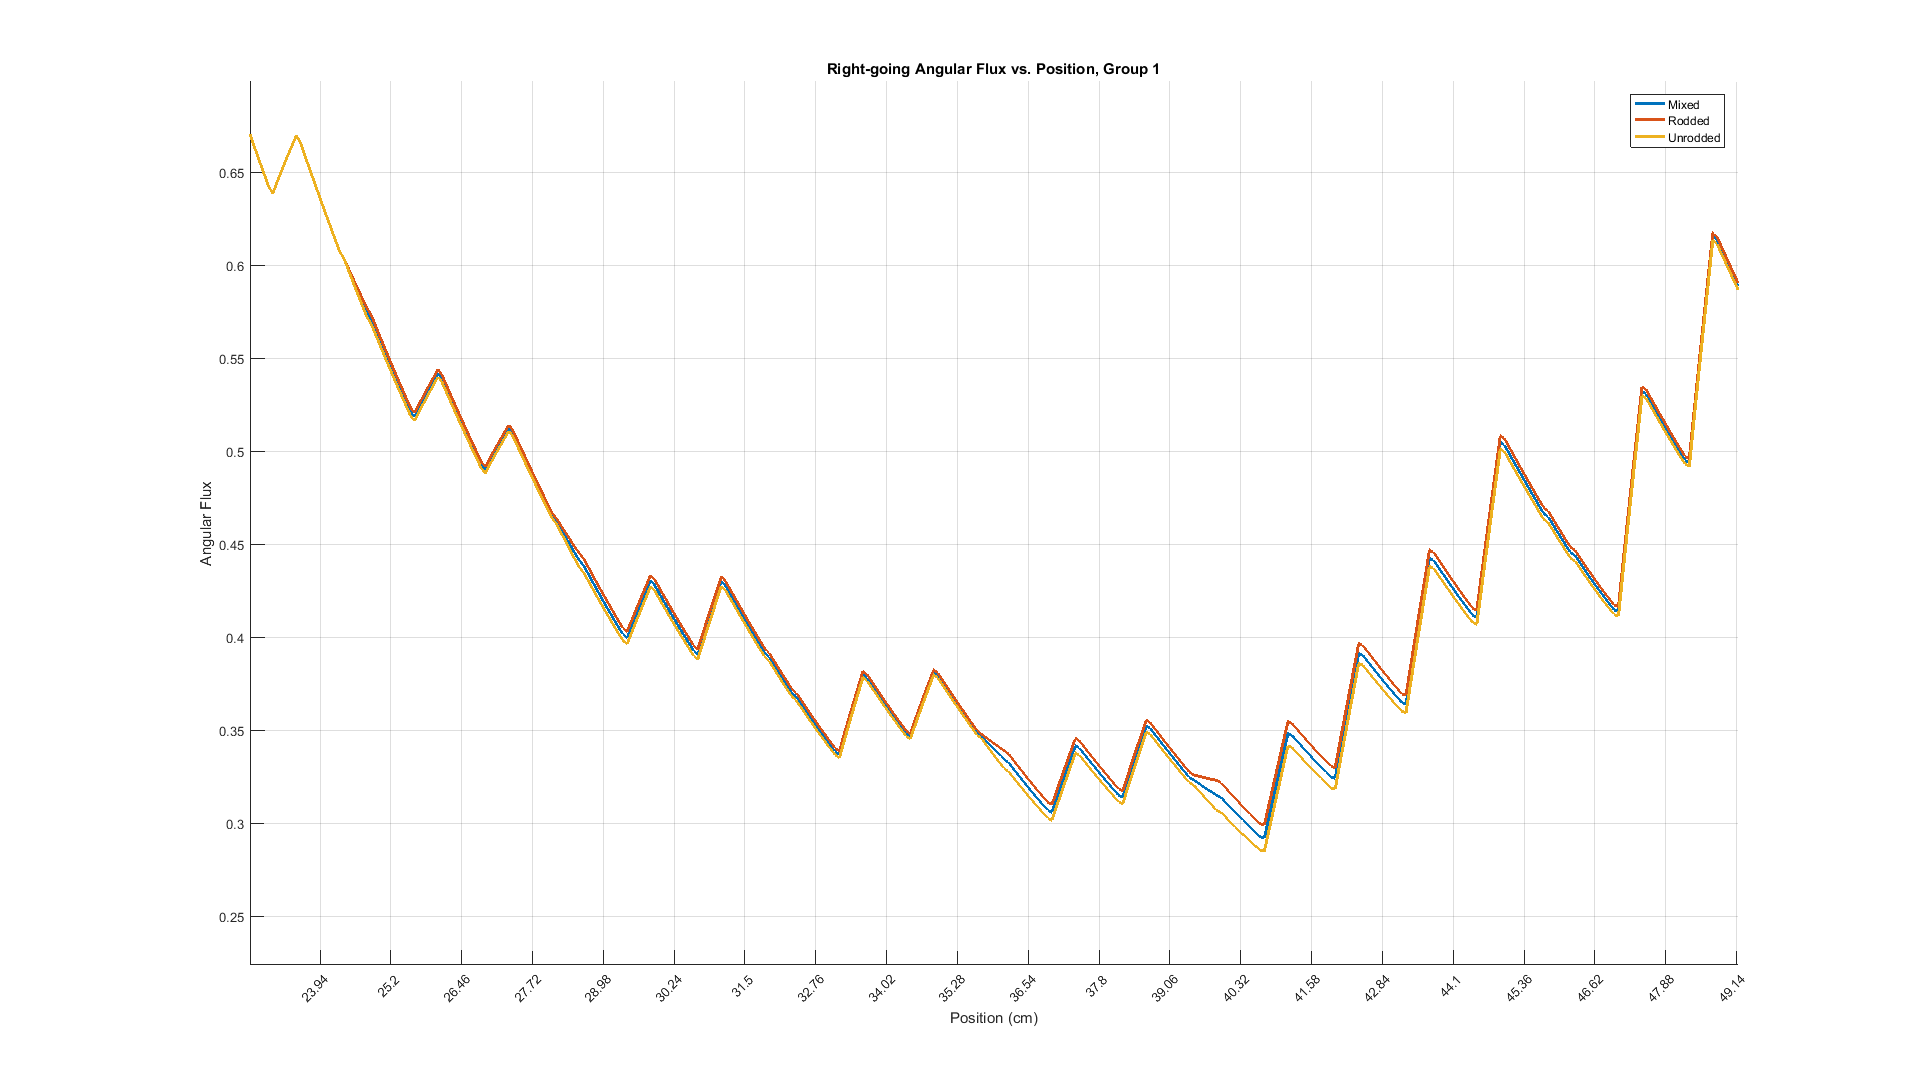
\includegraphics[width=0.6\textwidth]{1dmoc-50mix-fixedscat-angflux1.png}
        \label{f:1dmoc-fixed-50-angflux1}
    }
    ~
    \subfigure[Group 7]{
        \centering
        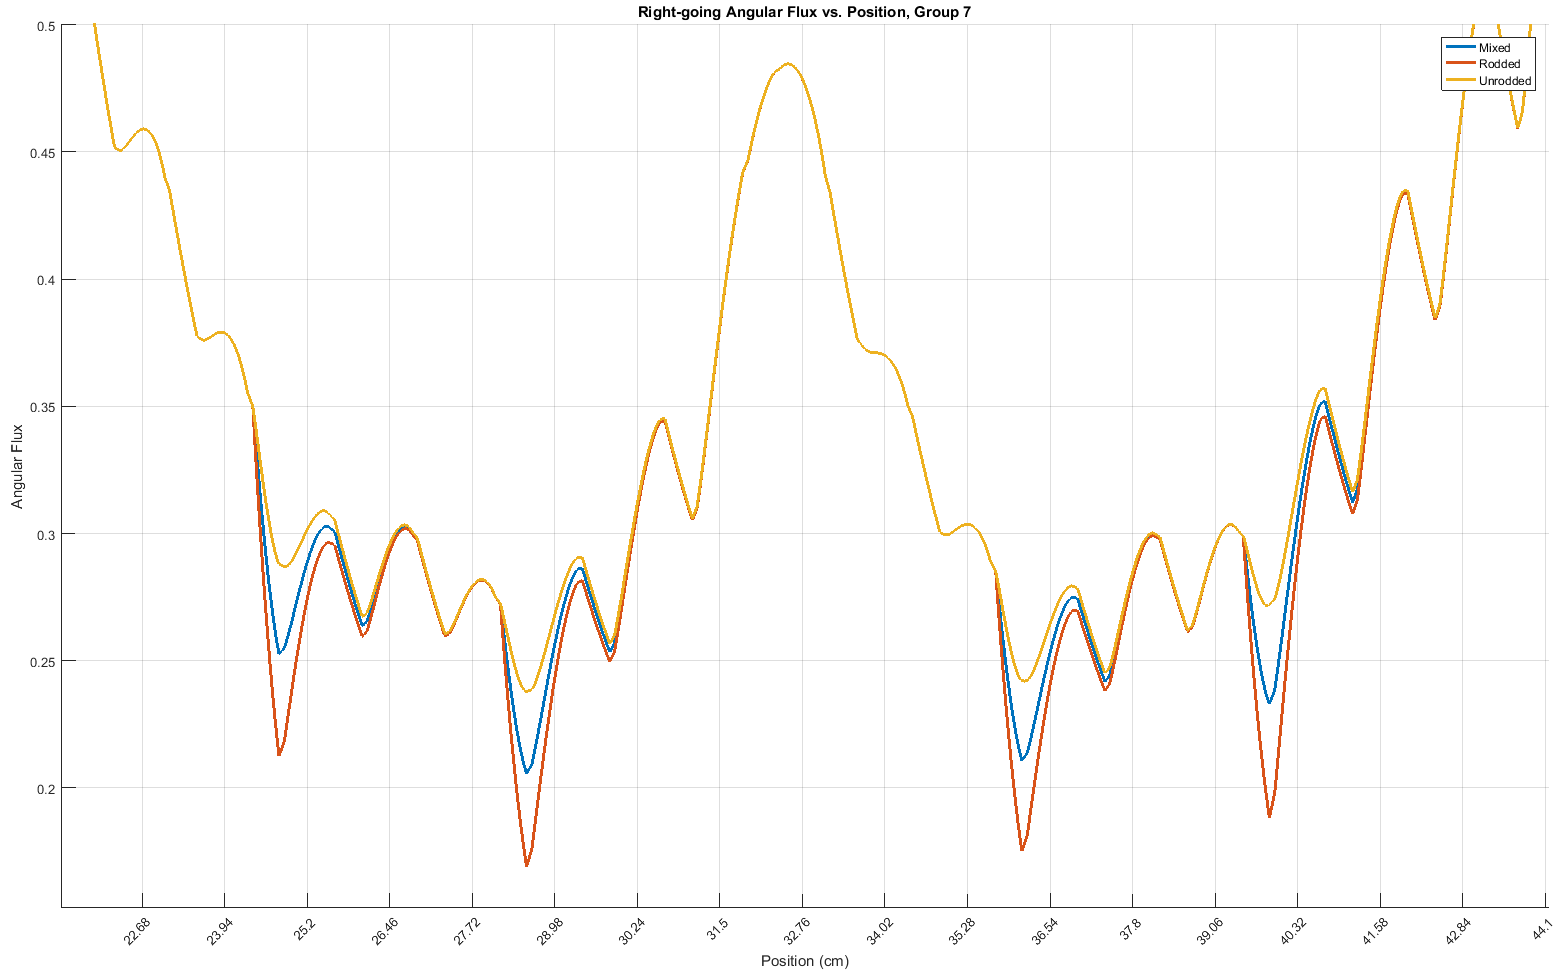
\includegraphics[width=0.6\textwidth]{1dmoc-50mix-fixedscat-angflux7.png}
        \label{f:1dmoc-fixed-50-angflux7}
    }
    \caption{Angular flux comparisons for a fixed fission and scattering source calculation}\label{f:1dmoc-fixed-50-angflux}
\end{figure}

The same cannot be said for the fast flux.  The mean free path of the fast flux is about 6.3 cm, which is the width of five pin cells.  Thus, it can be seen that each of the control rods after the first builds on the effects of the previous control rod.  While the fast flux does not have a significant impact on the fission source distribution, it does impact the scattering source distribution, which is not shown in these results.

\paragraph{Fixed Fission Source}

\begin{figure}[H]
    \centering
    \subfigure[25\% Mixture]{
        \centering
        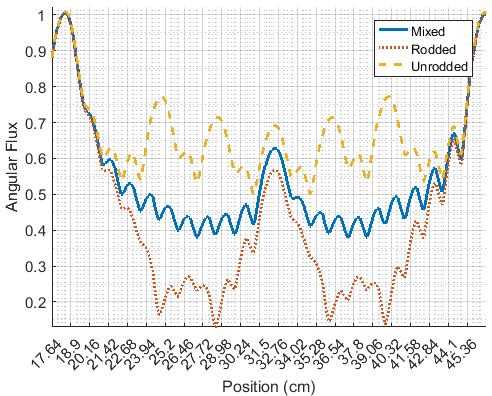
\includegraphics[width=0.45\textwidth]{1dmoc-25mix-angflux7.png}
        \label{f:1dmoc-25-angflux7}
    }
    \hfill
    \subfigure[50\% Mixture]{
        \centering
        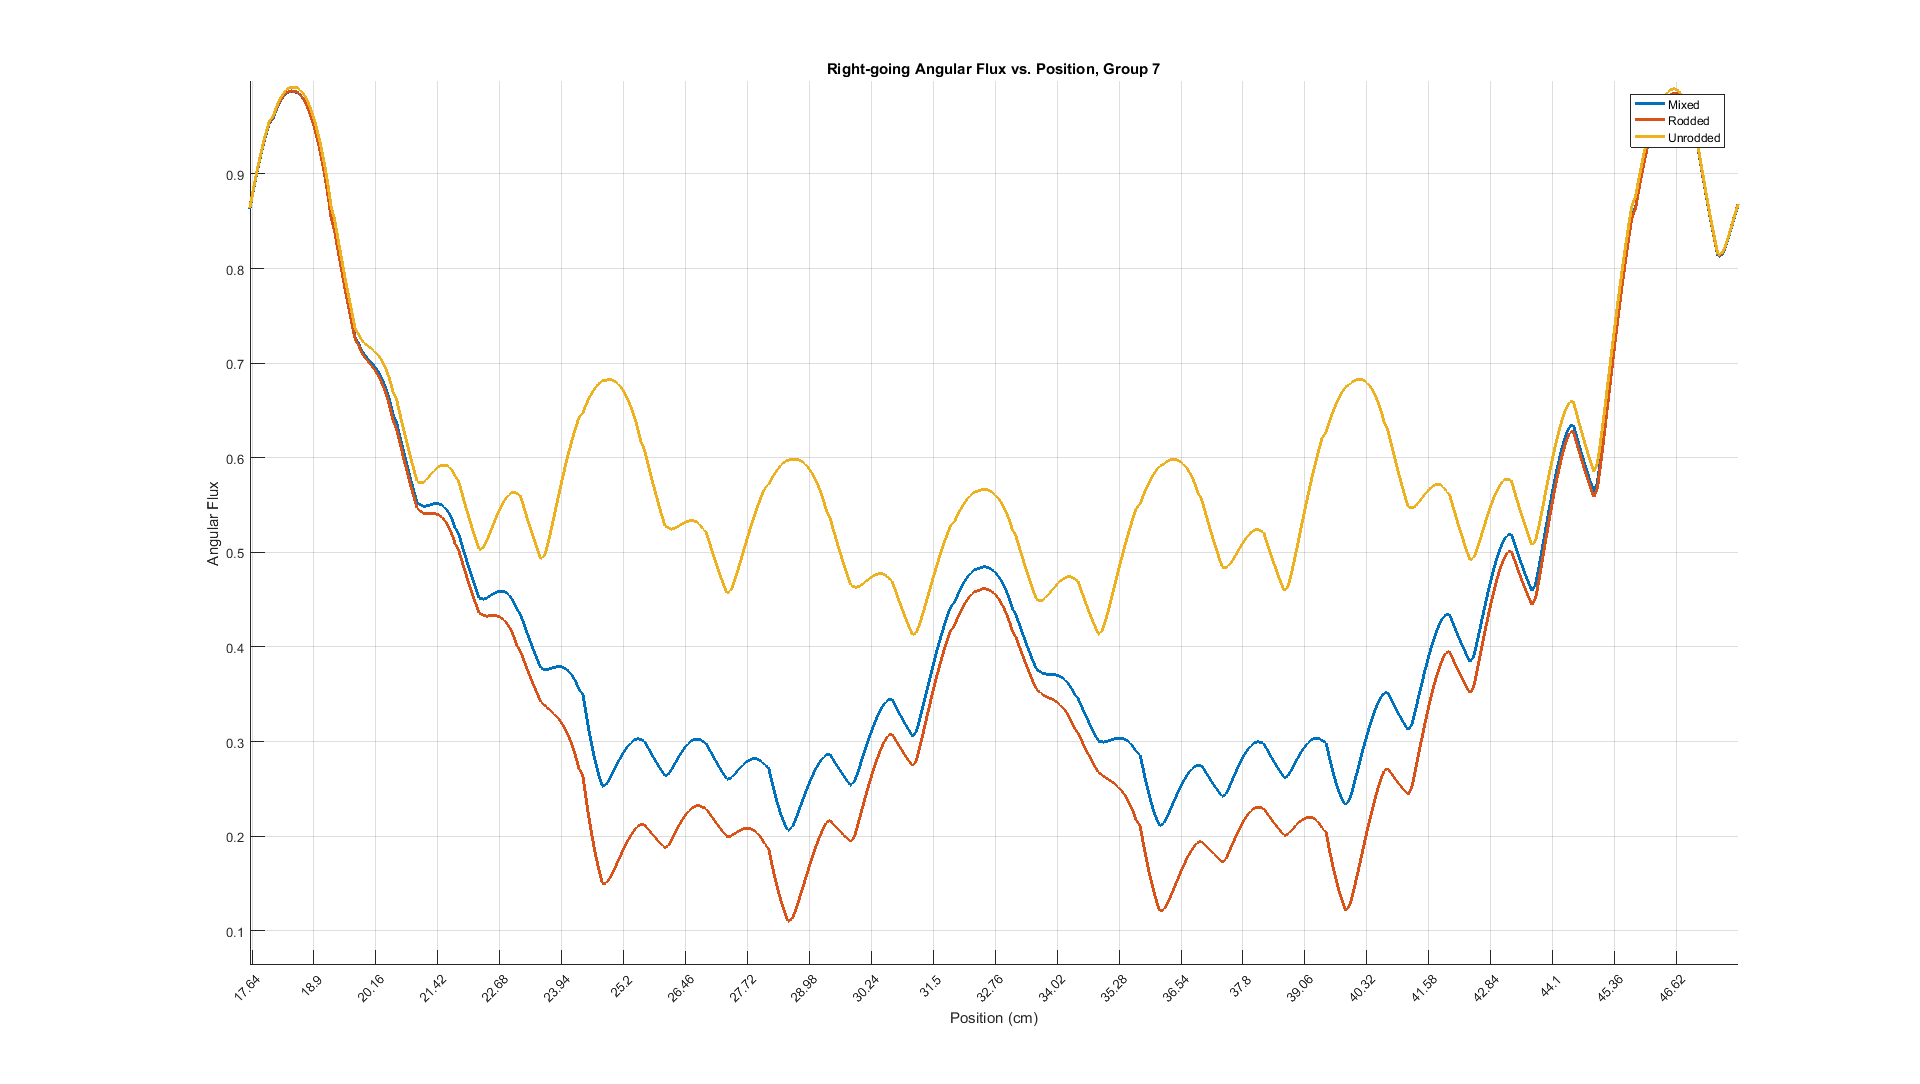
\includegraphics[width=0.45\textwidth]{1dmoc-50mix-angflux7.png}
        \label{f:1dmoc-50-angflux7}
    }
    ~
    \subfigure[75\% Mixture]{
        \centering
        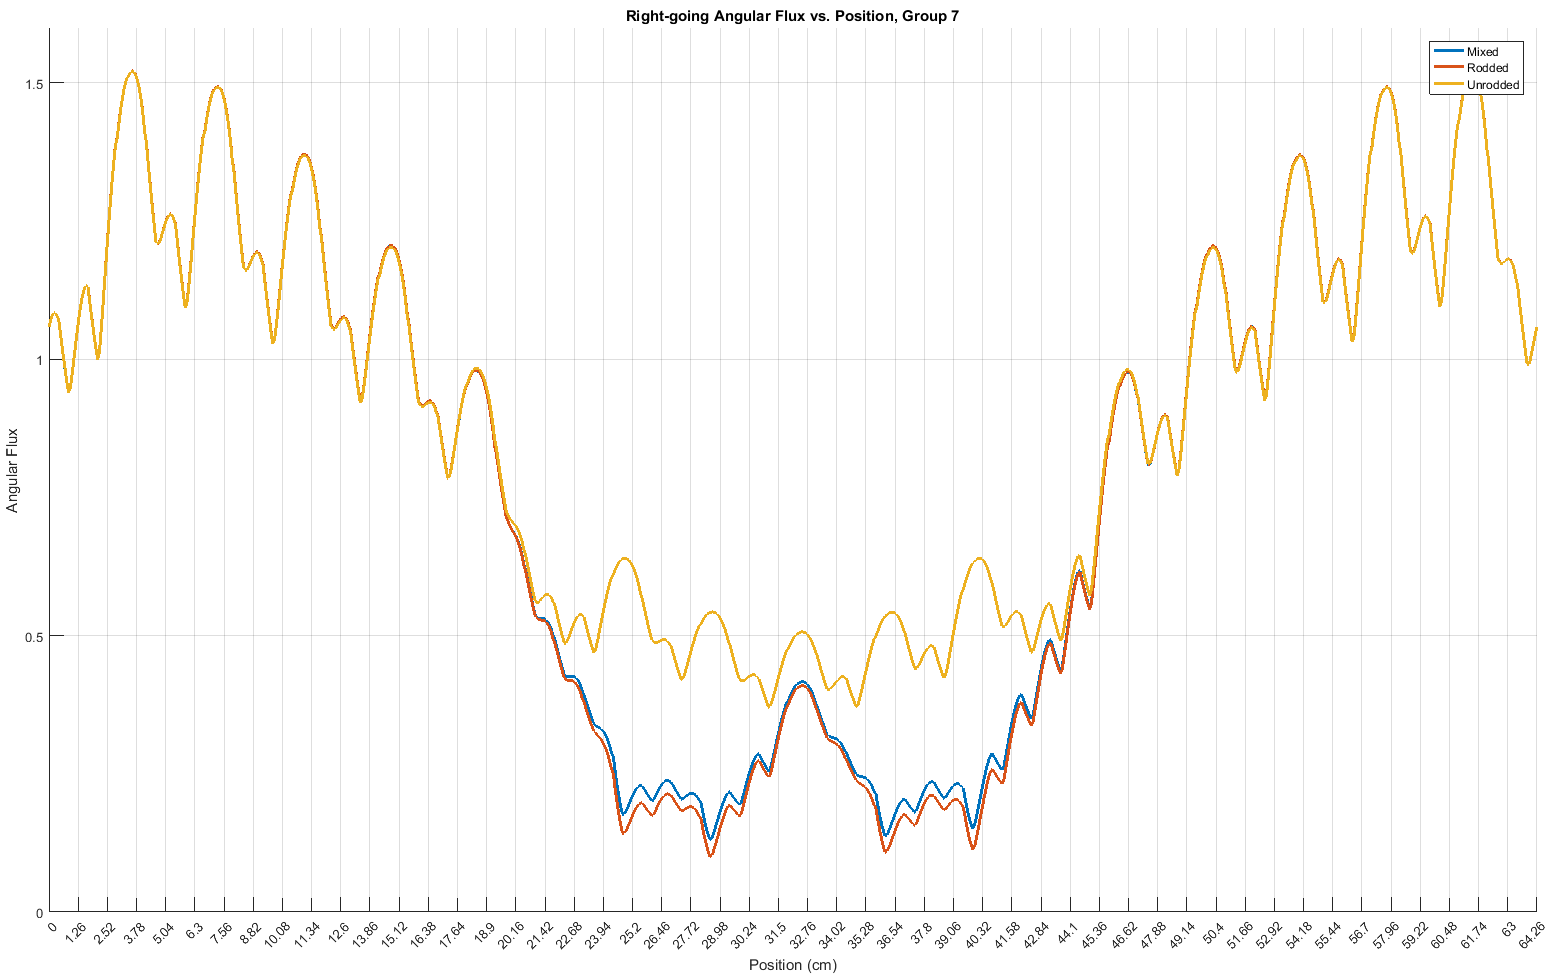
\includegraphics[width=0.45\textwidth]{1dmoc-75mix-angflux7.png}
        \label{f:1dmoc-75-angflux7}
    }
    \caption{Group 7 angular flux comparisons for 25\% and 75\% mixtures}\label{f:1dmoc-angflux7}
\end{figure}

The second set of calculations that was performed used a fixed fission source, but allowed the scattering source to fully converge for each calculation.  As in the previous section, an eigenvalue calculation was completed using partially rodded cross-sections.  This was done for 25\%, 50\%, and 75\% rodded cases.  For each case, a fixed fission source calculation was done with the fully rodded and fully unrodded cross-sections.  This time, multiple iterations were allowed for each material to converge the scattering source.  This allows us to see the effects of the rod on the scattering source distribution without worrying about changes in the eigenvalue and fission source distribution.

\begin{figure}[H]
    \centering
    \subfigure[25\% Mixture]{
        \centering
        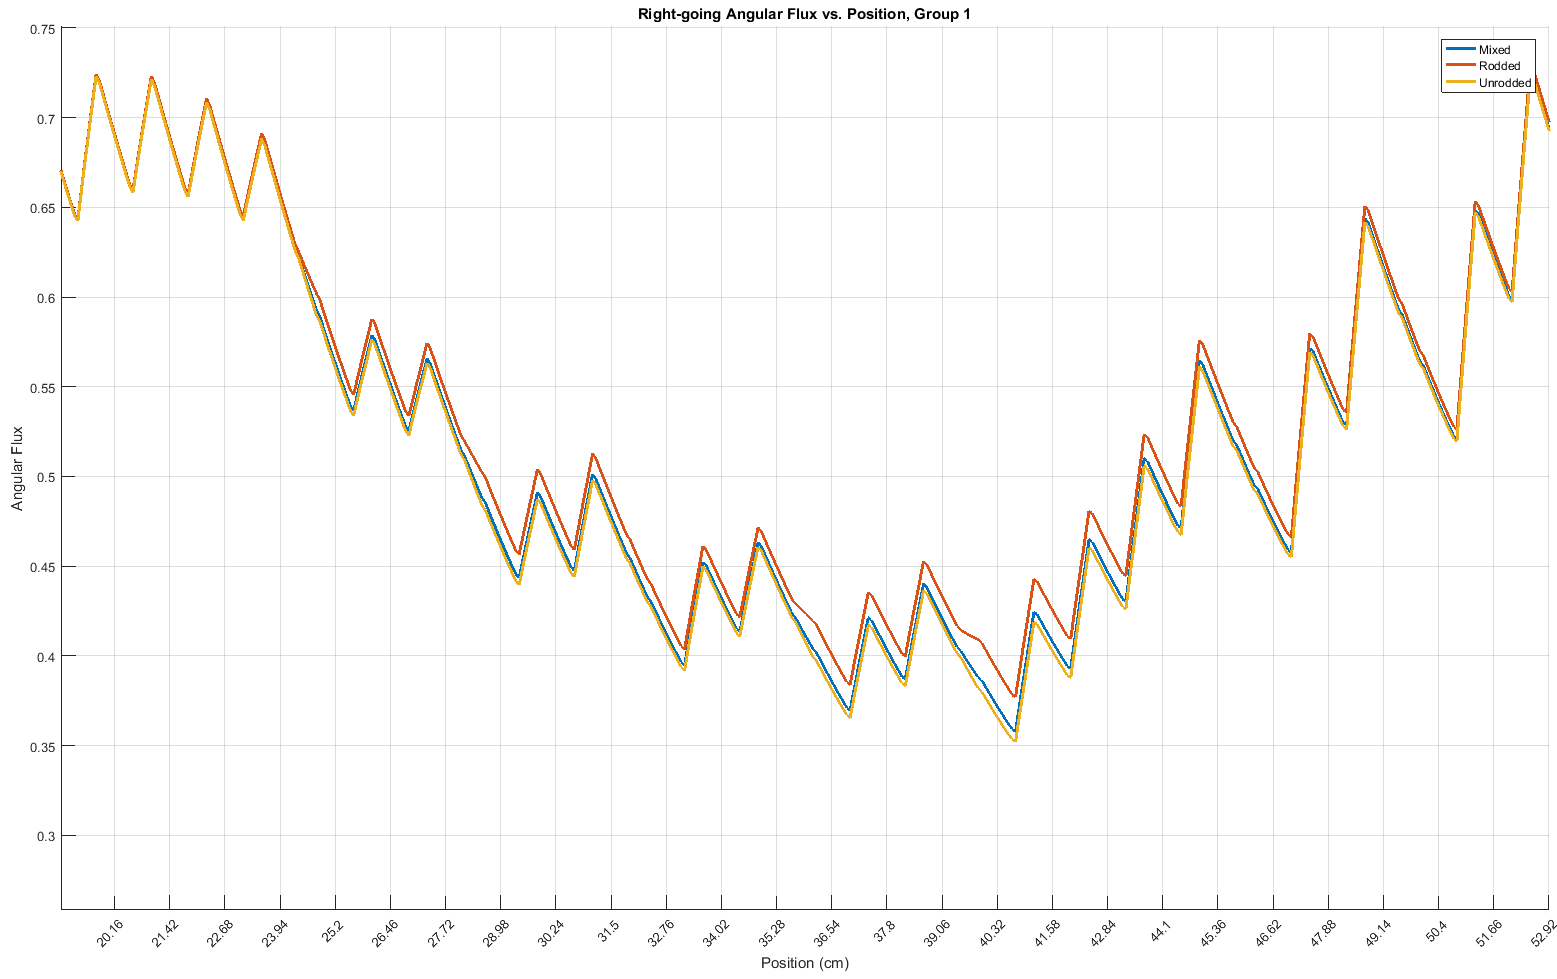
\includegraphics[width=0.45\textwidth]{1dmoc-25mix-angflux1.png}
        \label{f:1dmoc-25-angflux1}
    }
    \hfill
    \subfigure[50\% Mixture]{
        \centering
        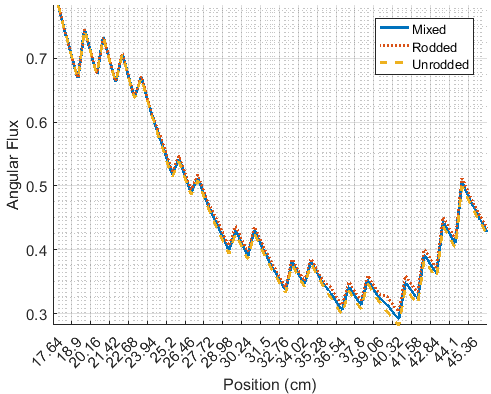
\includegraphics[width=0.45\textwidth]{1dmoc-50mix-angflux1.png}
        \label{f:1dmoc-50-angflux1}
    }
    ~
    \subfigure[75\% Mixture]{
        \centering
        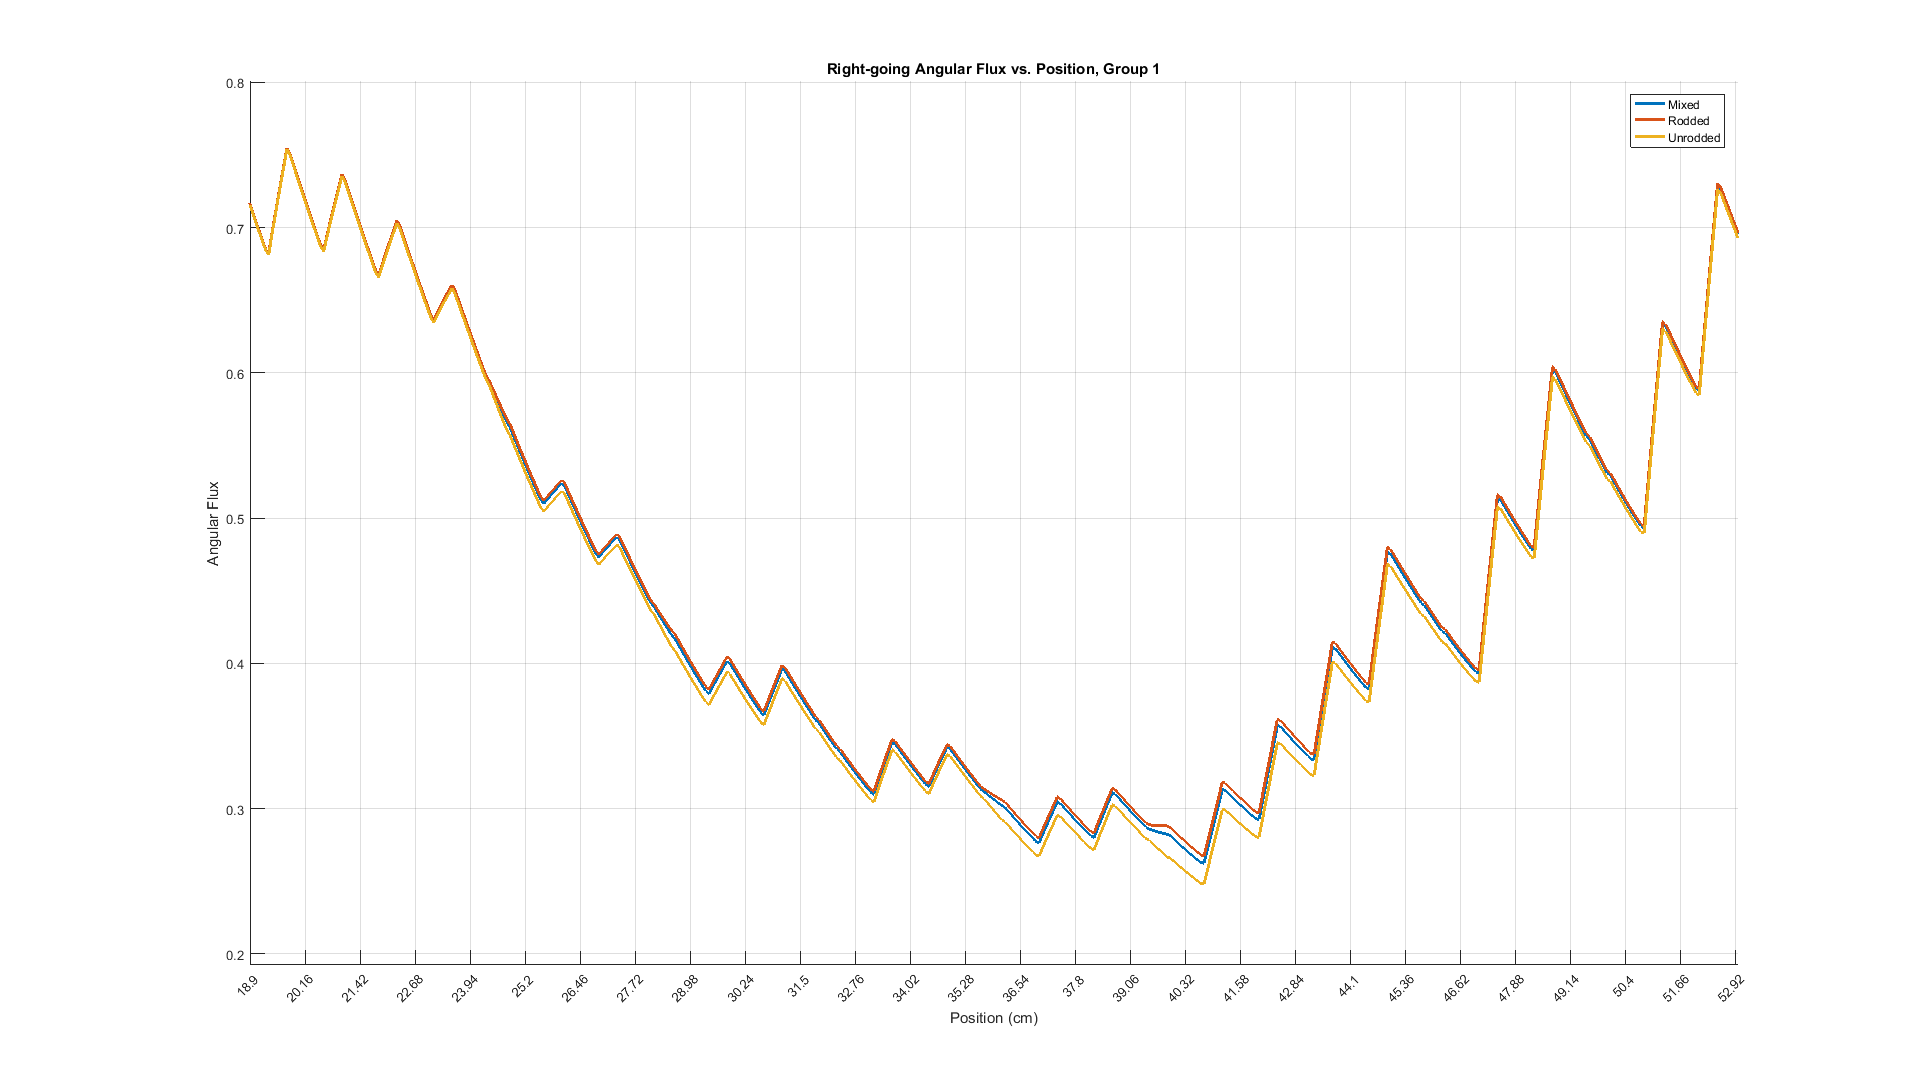
\includegraphics[width=0.45\textwidth]{1dmoc-75mix-angflux1.png}
        \label{f:1dmoc-75-angflux1}
    }
    \caption{Group 1 angular flux comparisons for 25\% and 75\% mixtures}\label{f:1dmoc-angflux1}
\end{figure}


Figure \ref{f:1dmoc-angflux7} shows the group 7 angular flux comparisons for each of the three mixtures.  We immediately see that for each of them, the angular flux for the mixture is closer to the rodded result than the unrodded result than what might be expected based on the volume fraction of the rod.  For example, comparing Figures \ref{f:1dmoc-50-angflux7} and \ref{f:1dmoc-fixed-50-angflux7} shows that the angular flux is much closer to the rodded solution than when the scattering source was fixed, despite the small mean free path of thermal neutrons.  Figure \ref{f:1dmoc-angflux1} shows the same comparisons for the group 1 angular flux.  While the difference in magnitude between each of the three cases is small for any mixture, the long mean free path means that these differences get spread out over a larger area.  This changes the shape of the scattering source for the thermal groups, which then has a more widespread effect on the the scalar flux distribution.  It should be noted as well that all angular flux plots shown here are for the flattest polar angle.  Since the steeper angles travel through more material in each region, the differences between them go away more quickly.  Thus, the angle shown in these plots is the one having the largest impact on the solution.

\subsection{Subray MOC Description}

\section{Results}
This chapter will present the results of calculations using each of the decusping methods described in the previous chapter.  First, results for the polynomial and subplane collision probabilities methods will be presented.  The subplane collision probabilities results are presented as two sets of data: one with just subplane (axial correction only) and one with both subplane and CP (axial and radial), allowing the difference in magnitude between the axial and radial effects of the rod to be determined.  These methods were tested using the VERA Progression Problems \cite{VERAProgressionProblems}, a series of benchmark problems based on the Watts Bar Unit 1 \hl{cite} reactor that provide realistic test cases for the 2D/1D methods.  The control rods in these models were moved to various locations that stress the mesh typically used by MPACT to solve these problems, allowing the benefit of the decusping techniques to be clearly seen.  For some of these problems, detailed 3D power distributions were generated using the Monte Carlo code KENO-VI \hl{cite}, allowing for comparisons of the decusping methods with both refined MPACT meshes and Monte Carlo reference solutions.

In the second half of the chapter, results for the subray method of characteristics will be presented.  The first set of results come from the 1D prototype code discussed in Section \ref{ss:1dcode}.  This code provided a quick implementation to show that it was worth pursuing the method in a full-scale transport code.  After this, results from MPACT's implementation of subray MOC will be presented for both 2D and 3D problems.  These results will be compared to refined mesh solutions in MPACT as well as the polynomial and subplane collision probabilities solutions to determine the relative accuracy of each of these methods.  All subray MOC results will use the C5G7 benchmark problems \cite{EELewisC5G72003,EELewisC5G7extended2005}.  Because these problems have specified macroscopic cross sections, some of the complexities of cross section processing and shielding calculations for subray MOC can be deferred to later research while still examining the accuracy and performance of subray MOC compared with other solutions to the rod cusping problem.

\section{VERA Problem 4}\label{s:vera4}

\begin{figure}[h]\label{f:p4layout}
    \centering
    \subfigure{\label{f:p4radial}
        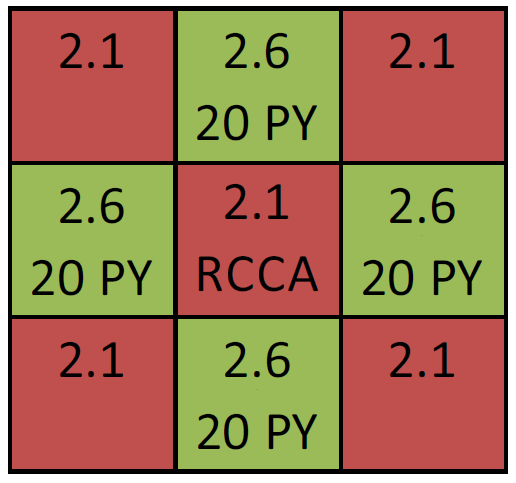
\includegraphics[width=0.4\textwidth]{p4a_layout.png}
    }
    ~
    \subfigure{\label{f:p4axial}
        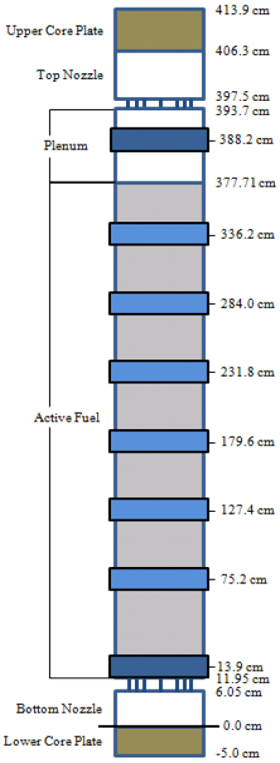
\includegraphics[width=0.3\textwidth]{wb_3d_assembly.png}
    }
    \caption{VERA Problem 4 radial (left) and axial (right) layouts}\label{f:p4}
\end{figure}

VERA Progression Problem 4 is composed of a 3x3 set of Westinghouse 17$\times$17 fuel assemblies with an active fuel height of 365.76 cm and a control bank in the center assembly.  The radial layout of the problem is shown in Figure \ref{f:p4radial}, and the axial layout of each assembly is shown in Figure \ref{f:p4axial}.  The control rods were placed at an axial elevation of 257.9 cm above the core plate, about one third inserted into the core.  The rod in the original problem specification is made of AIC with a \bfc{} follower and a stainless steel tip.  First, results will be presented which use several difference uniform rods to simplify the analysis, then results will be presented with the heterogeneous rod.  Lastly, a differential rod worth developed with the heterogeneous rod is shown with comparisons to KENO-VI reference solutions at regular intervals along the curve.

\subsection{Homogeneous Control Rods}

For the reference solution, 58 MOC planes were used with 49 of them in the active fuel region.  It was also ensured that the end of the control rods were exactly aligned with one of the MOC plane boundaries.  The cases with decusping methods used the same mesh, but with the 2 MOC planes around the tip of the control rod merged into a single plane to introduce cusping effects.  The accuracy and convergence data for these cases are shown in Table \ref{t:homoDecusp}.

\begin{table}[ht]
    \centering
    \caption{Comparison of Rod Decusping Methods in MPACT for VERA Progression 
        Problem 4 for Homogeneous Control Rods}
    \resizebox{\textwidth}{!}{\begin{tabular}{l l S[table-format=3.1,table-number-alignment=left] 
            S[table-format=1.2,table-number-alignment=left] 
            S[table-format=2.2,table-number-alignment=left] 
            S[table-format=2.1,table-number-alignment=left] l}\toprule
        Rod & \multirow{2}{*}{{Case}} & {\keff{}} & 
        \multicolumn{2}{l}{{Pin Power 
                Differences}} & \multirow{2}{*}{{2D/1D Iterations}} & {Runtime}\\
        Material & & {Difference (pcm)} & {RMS} & {Max} &  & {(Core-Hours)} \\\midrule
        \multirow{5}{*}{AIC}      & Reference        & {--}  &    {--} &     {--} & 15 & 19.6 \\
                                  & No treatment     & -29.5 & 1.53\% & 11.84\% & 12 & 14.7 \\
                                  & Polynomial       &  -0.3 & 0.44\% &  4.08\% & 12 & 14.3 \\
                                  & Subplane         & -11.5 & 0.73\% &  8.21\% & 12 & 14.2 \\
                                  & Subplane + CP    &  -5.6 & 0.37\% &  4.25\% & 12 & 15.3\\\midrule
        \multirow{5}{*}{\bfc{}}   & Reference        & {--}  &    {--} &     {--} & 15 & 16.9 \\
                                  & No treatment     & 112.0 & 6.98\% & 69.37\% & 12 & 12.7 \\
                                  & Polynomial       & 112.6 & 6.89\% & 66.73\% & 12 & 12.1 \\
                                  & Subplane         & -17.9 & 1.14\% & 11.36\% & 13 & 15.2 \\
                                  & Subplane + CP & -11.0 & 0.69\% &  6.37\% & 12 & 13.4 \\\midrule
        \multirow{5}{*}{Tungsten} & Reference        & {--}  & {--}   &      {--} & 15 & 23.5 \\
                                  & No treatment     &  -8.4 & 0.37\% &  3.37\% & 12 & 15.5 \\
                                  & Polynomial       &  -4.4 & 0.24\% &  2.72\% & 12 & 14.5 \\
                                  & Subplane         &   1.6 & 0.07\% &  0.60\% & 12 & 13.9 \\
                                  & Subplane + CP    &  -0.9 & 0.06\% &  0.94\% & 12 & 15.6 \\\bottomrule
    \end{tabular}}
    \label{t:homoDecusp}
\end{table}

The ``No Treatment'' cases show the magnitude of the cusping effects for each of the rod types.  The largest cusping errors occur for the \bfc{} rod, which is a strong thermal absorber.  For this rod, the polynomial treatment has very little effect, leaving large errors in the solution.  The subplane method reduces the error in \keff{} to an almost negligible -18 pcm, but still leaves significant power distribution errors of 1.14\% RMS and 11.36\% Max.  Introduing the 1D CP calculations brings the maximum error below 7\%.  These results indicate that the polynomial method is not capable of accurately resolving the \bfc{} rod.  Because it is a strong thermal absorber, smearing the rod material throughout the plane at all introduces large errors that cannot be correct just by reducing the volume fraction.  The subplane-based methods are both able to resolve the rod more accurately since they actually modify the cross sections used in the CMFD and P$_3$ calculations.

For the AIC rod, the polynomial correction performs much better than for the \bfc{} rod, reducing the maximum error from 12\% to 4\%.  The subplane treatment only reduces the error to 8.21\%, while adding the CP calculations reduces the errors to about the same point as the polynomial treatment.  The AIC rod has resonance absorption and is not as strongly absorbing in the thermal energy ranges as the \bfc{} rod, causing some differences in behavior of these methods.  The polynomial method does a better job with the AIC rod since the complex effects are accounted for in the polynomial generation.  However, the subplane treatment does not perform well since it does nothing to account for the radial effects of the AIC rod.  For both rod types, the subplane treatment with radial CP calculations performs well since it is able to capture both radial and axial effects of the rod.

For the tungsten rod, the errors are not nearly as high as for the AIC or \bfc{} rods.  However, the subplane-based treatments still perform significantly better than the polynomial treatment, bringing the \keff{} error to negligible levels and reducing the maximum power errors under 1\%.

For all 3 rod types, Table \ref{t:homoDecusp} also shows the convergence and runtime data for each calculation.  The decusping treatments consistently converge in fewer iterations than the reference.  This is due to the fact that the reference has an additional thin MOC plane that the other cases do not have.  This thin plane requires underrelaxation for 2D/1D to converge, causing a small increase in the number of 2D/1D iterations required.  Because of the difference in iterations, all decusping methods also require less runtime by about 25\% on average.  The subplane-based methods are generally a bit slower than the polynomial method, despite requiring the same number of 2D/1D iterations.  The reason for this is that the subplane-based methods modify the CMFD system, which results in more CMFD inner iterations to converge during each outer 2D/1D iteration.  This increases the total runtime of the problem even though 2D/1D itself converges the same.  However, in most cases the trade-off between runtime and accuracy would favor the use of the subplane-based 

\subsection{Heterogeneous Control Rod}

Next, the same set of results can be shown again, but with the heterogeneous rod.  The same 58-plane reference mesh was used for these results.  However, the decusping cases have only 55 planes instead of 57.  Three additional planes are eneded in the reference case to account for all three material interfaces in the heterogeneous rod: \bfc{}/AIC, AIC/SS, and SS/moderator.  The decusping methods are applied at all three of these locations simultaneously, with the exception of the SS/moderator interface for the polynomial decusping since there is no SS polynomial data.  The results are shown in Table \ref{t:hetDecusp}.

\begin{table}[ht]
    \centering
    \caption{Comparison of Rod Decusping Methods in MPACT for VERA Progression 
        Problem 4 for Heterogeneous Control Rod}
    \begin{tabular}{l S[table-format=2.1,table-number-alignment=left] l 
            S[table-format=2.3,table-number-alignment=left] l l}\toprule
        \multirow{2}{*}{Case} & {\keff{}} & \multicolumn{2}{l}{{Pin Power 
                Differences}} & \multirow{2}{*}{{2D/1D Iterations}} & {Runtime}\\
        & {Difference (pcm)} & {RMS} & {Max} &  & {(Core-Hours)} \\\midrule
        Reference        &  {--} &    {--} &     {--} & 15 & 16.6 \\
        No treatment     & -45.9 & 2.43\% & 20.45\% & 12 & 13.8 \\
        Polynomial       &  -2.5 & 0.46\% &  5.07\% & 12 & 13.0 \\
        Subplane         & -17.3 & 1.10\% & 11.77\% & 13 & 14.9 \\
        Subplane + CP    &  -5.5 & 0.42\% &  3.87\% & 12 & 14.7 \\\bottomrule
    \end{tabular}
    \label{t:hetDecusp}
\end{table}

With no treatment, the maximum error is over 20\%.  The oplynomial method performs wells, reducing the error to about 5\%, with an RMS power error under 0.5\% and \keff{} error of -2.5 pcm.  This behavior is consistent with what is expected based on the homogeneous results.  The primary location of rod cusping effects is at the AIC/SS interface, and the errors obtained from the polynomial decusping method are comparable to those observed in the homogeneous AIC rod calculations.  Following this trend, the subplane treatment without radial CP does not perform as well as the polynomial treatment, reducing the maximum error to just under 12\%.  Finally, the subplane treatment with radial CP generates the most accurate results, with a maximum power error under 4\%.  This method makes no assumptions about which materials are next to each other, can handle all three control rod materials, and accounts for both radial and axial effects of the rod, making it the most consistent and accurate of the methods across a variety of cases.

The trends in the convergence and runtime data are similar to those observed with the homogeneous rods.  The decusping treatment calculations take fewer 2D/1D iterations because fewer thin planes are used in the model, requiring less underrelaxation than the reference case.  Furthermore, some increase in runtime is seen in the subplane-based methods over the polynomial method due to changes in the convergence of the CMFD system during each 2D/1D iteration.  The CP calculations themselves are negligible since they consist only of inverting an 8$\times$8 matrix for each energy group, which can be done very quickly.  Again, the trade-off between runtime and accuracy for this problem favors using the subplane treatment with radial CP if the fine mesh solution's accuracy is not required.

\subsection{Differential Rod Worth Curve}

\begin{figure}[h]
    \centering
    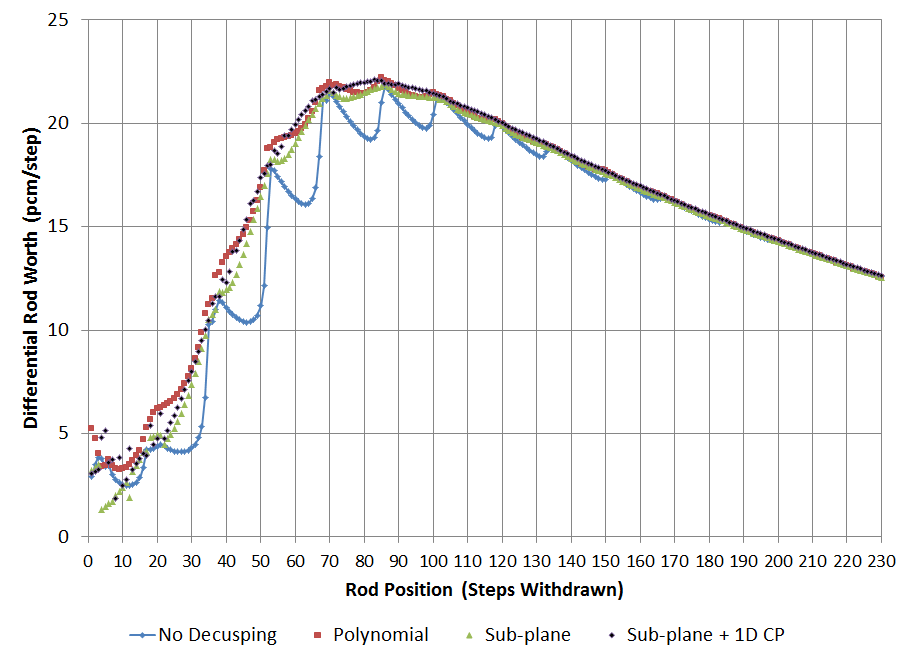
\includegraphics[width=\textwidth]{../../figs/differentialRodworth.png}
    \caption{Differential rod worth curves for MPACT decusping 
        techniques.}\label{f:rodworth}
\end{figure}

To show the effectiveness of each decusping technique as the rod moves upward through the reactor, a differential rod worth curve was developed for each method.  This curve is shown in Figure \ref{f:rodworth}.  With no decusping method, the errors in the rodworth approach 50\% at some positions.  The polynomial treatment greatly reduces these errors, but does not fully smooth the curve.  Especially near the peak of the curve, some oscillation about the true solution can be seen when using the polynomial treatment.  The subplane treatment behaves similarly to the polynomial treatment, but with slightly larger errors in most places.  Finally, adding the radial CP calculations generates a smooth curve at almost every rod position.

The exception to the good behavior of the subplane + CP method occurs when the rod is almost fully inserted.  At such positions, all methods fail to produce a smooth rod worth curve due to the severe power shape.  The polynomial method is always limited in its ability to resolve the partially inserted rod if the local power shape differs significantly from the one with which the polynomial data was generated.  The subplane-based treatments struggle with the fully inserted rod because each subplane in an MOC plane uses the same MOC solution data for the CMFD and P$_3$ solutions.  In the cases where MOC planes are near both the control rod tip and the boundary of the problem, the radial solution is changing more quickly than normal and cannot be resolved as well by the subplane scheme.

\subsection{KENO-VI Comparisons}

\begin{table}[h]
    \centering
    \caption{Average Differences between MPACT and KENO-VI for VERA Problem 
        4}\label{t:keno}
    \sisetup{separate-uncertainty=true,table-text-alignment=left,table-number-alignment=left}
    \begin{tabular}{l l 
            S[table-format=3.1,table-number-alignment=left] 
            S[table-format=1.3,table-number-alignment=left] 
            S[table-format=2.3,table-number-alignment=left]}\toprule
        \multirow{2}{*}{Cases} & \multirow{2}{*}{{Decusping Method}} & \multirow{2}{*}{{\keff{} 
                Difference}} & 
        \multicolumn{2}{l}{{Pin Power Difference}} \\
        &  &  & {RMS} & {Max} \\\midrule
        \multirow{4}{*}{Average}       & None              &   -24.9 &  5.380\% & 25.902\% \\
                                       & Polynomial        &    34.8 &  1.502\% &  8.957\% \\
                                       & Subplane          &    34.6 &  0.984\% &  4.597\% \\
                                       & Subplane + CP     &    41.4 &  0.763\% &  3.386\% 
        \\\midrule
        \multirow{2}{*}{Worst -- 20\%} & None              & -176.0 & 14.709\% & 63.929\% \\
                                       & Polynomial        & 13.9   &  3.344\% & 25.373\% \\
                                       & Subplane          & 9.6    &  1.921\% &  9.900\% \\
                                       & Subplane + CP     & 45.9   &  1.324\% &  4.921\% \\
        \midrule
        Fully Withdrawn                & --                & 40.5   & 0.34\%   & 1.493\% \\
        \bottomrule
    \end{tabular}
\end{table}

For the rod worth curves in the previous section, KENO-VI calculations were done in 10\% intervals along the curve, giving a total of 11 KENO-VI data sets that can be used as a reference for MPACT.  Each KENO-VI calculation was run for 1000 active generations, with \hl{number} particles per generation, for a total of \hl{number} particles contributing to the final solution and statistics.  The uncertainty in the KENO-VI results was about 1 pcm for the eigenvalue and less than 0.3\% for the power distribution.  While the uncertainty in the power distribution is a bit higher than would normally be used, it is more than sufficiently converged to discuss the relative accuracy of rod cusping treatments.  For the first ten sets of KENO-VI data along the curve, each decusping method was compared.  Table \ref{t:keno} shows the average results for all 10 of these points, along with results for the worst of the 10, which occurs at 20\% (46 steps withdrawn) where the differential rod worth curve is steepest.  The table also shows a comparison for the 100\% withdrawn data set.  This final data set occurs for the tip of the control rod above the top of the active fuel, so there are no cusping effects.  This serves to give an idea of how accurate MPACT is compared to Monte Carlo when there are no control rod cusping effects.

The fully withdrawn case shows that when no cusping effects are present, MPACT can be expected to have less than 0.5\% RMS power difference and approximately 1.5\% maximum power difference compared with a Monte Carlo solution.  When cusping is introduced, these errors jump to around 25\% on average, with a maximum error over 60\%.  For both the average and maximum cases, the polynomial treatment compares worst with KENO-VI and the subplane treatment with 1D CP performs best, reducing the maximum power errors to about 5\% in the worst case scenario.  While these errors are still larger than desired for 2D/1D, they are much closer to acceptable levels than some of the 20-30\% errors observed in many calculations.  However, these KENO-VI comparisons do indicate that use of the polynomial decusping treatment should be restricted to specific cases in which it is known to perform well.  Using it for everything could easily and unknowingly result in unacceptably large errors in the 2D/1D solution.

\section{VERA Problem 5}

To demonstrate the behavior of the decusping methods on a full-core problem, VERA Problem 5 was also run.  Problem 5 is the a beginning-of-cycle simulation of the Watts Bar Unit 1 PWR.  The model of this reactor uses the same axial layout shown in Figure \ref{f:p4axial} with the radial layout shown in Figure \ref{f:p5radial}.  For these calculations, Bank D was set to a position of 257.9 cm above the core plate while all other banks were fully withdrawn to 383.3125 cm, about 6 cm above the top of the active fuel.

Like problem 4, the reference case was run with 58 planes while the decusping cases were run with 57 planes.  Radial decomposition was used with 16 cores per MOC plane.  This resulted in a slightly different number of cores for the reference case compared with the others, as seen in the Problem 4 calculations.  The accuracy and convergence results for the partially rodded plane are shown in Table \ref{t:p5decusp}.

\begin{figure}[h]
\centering
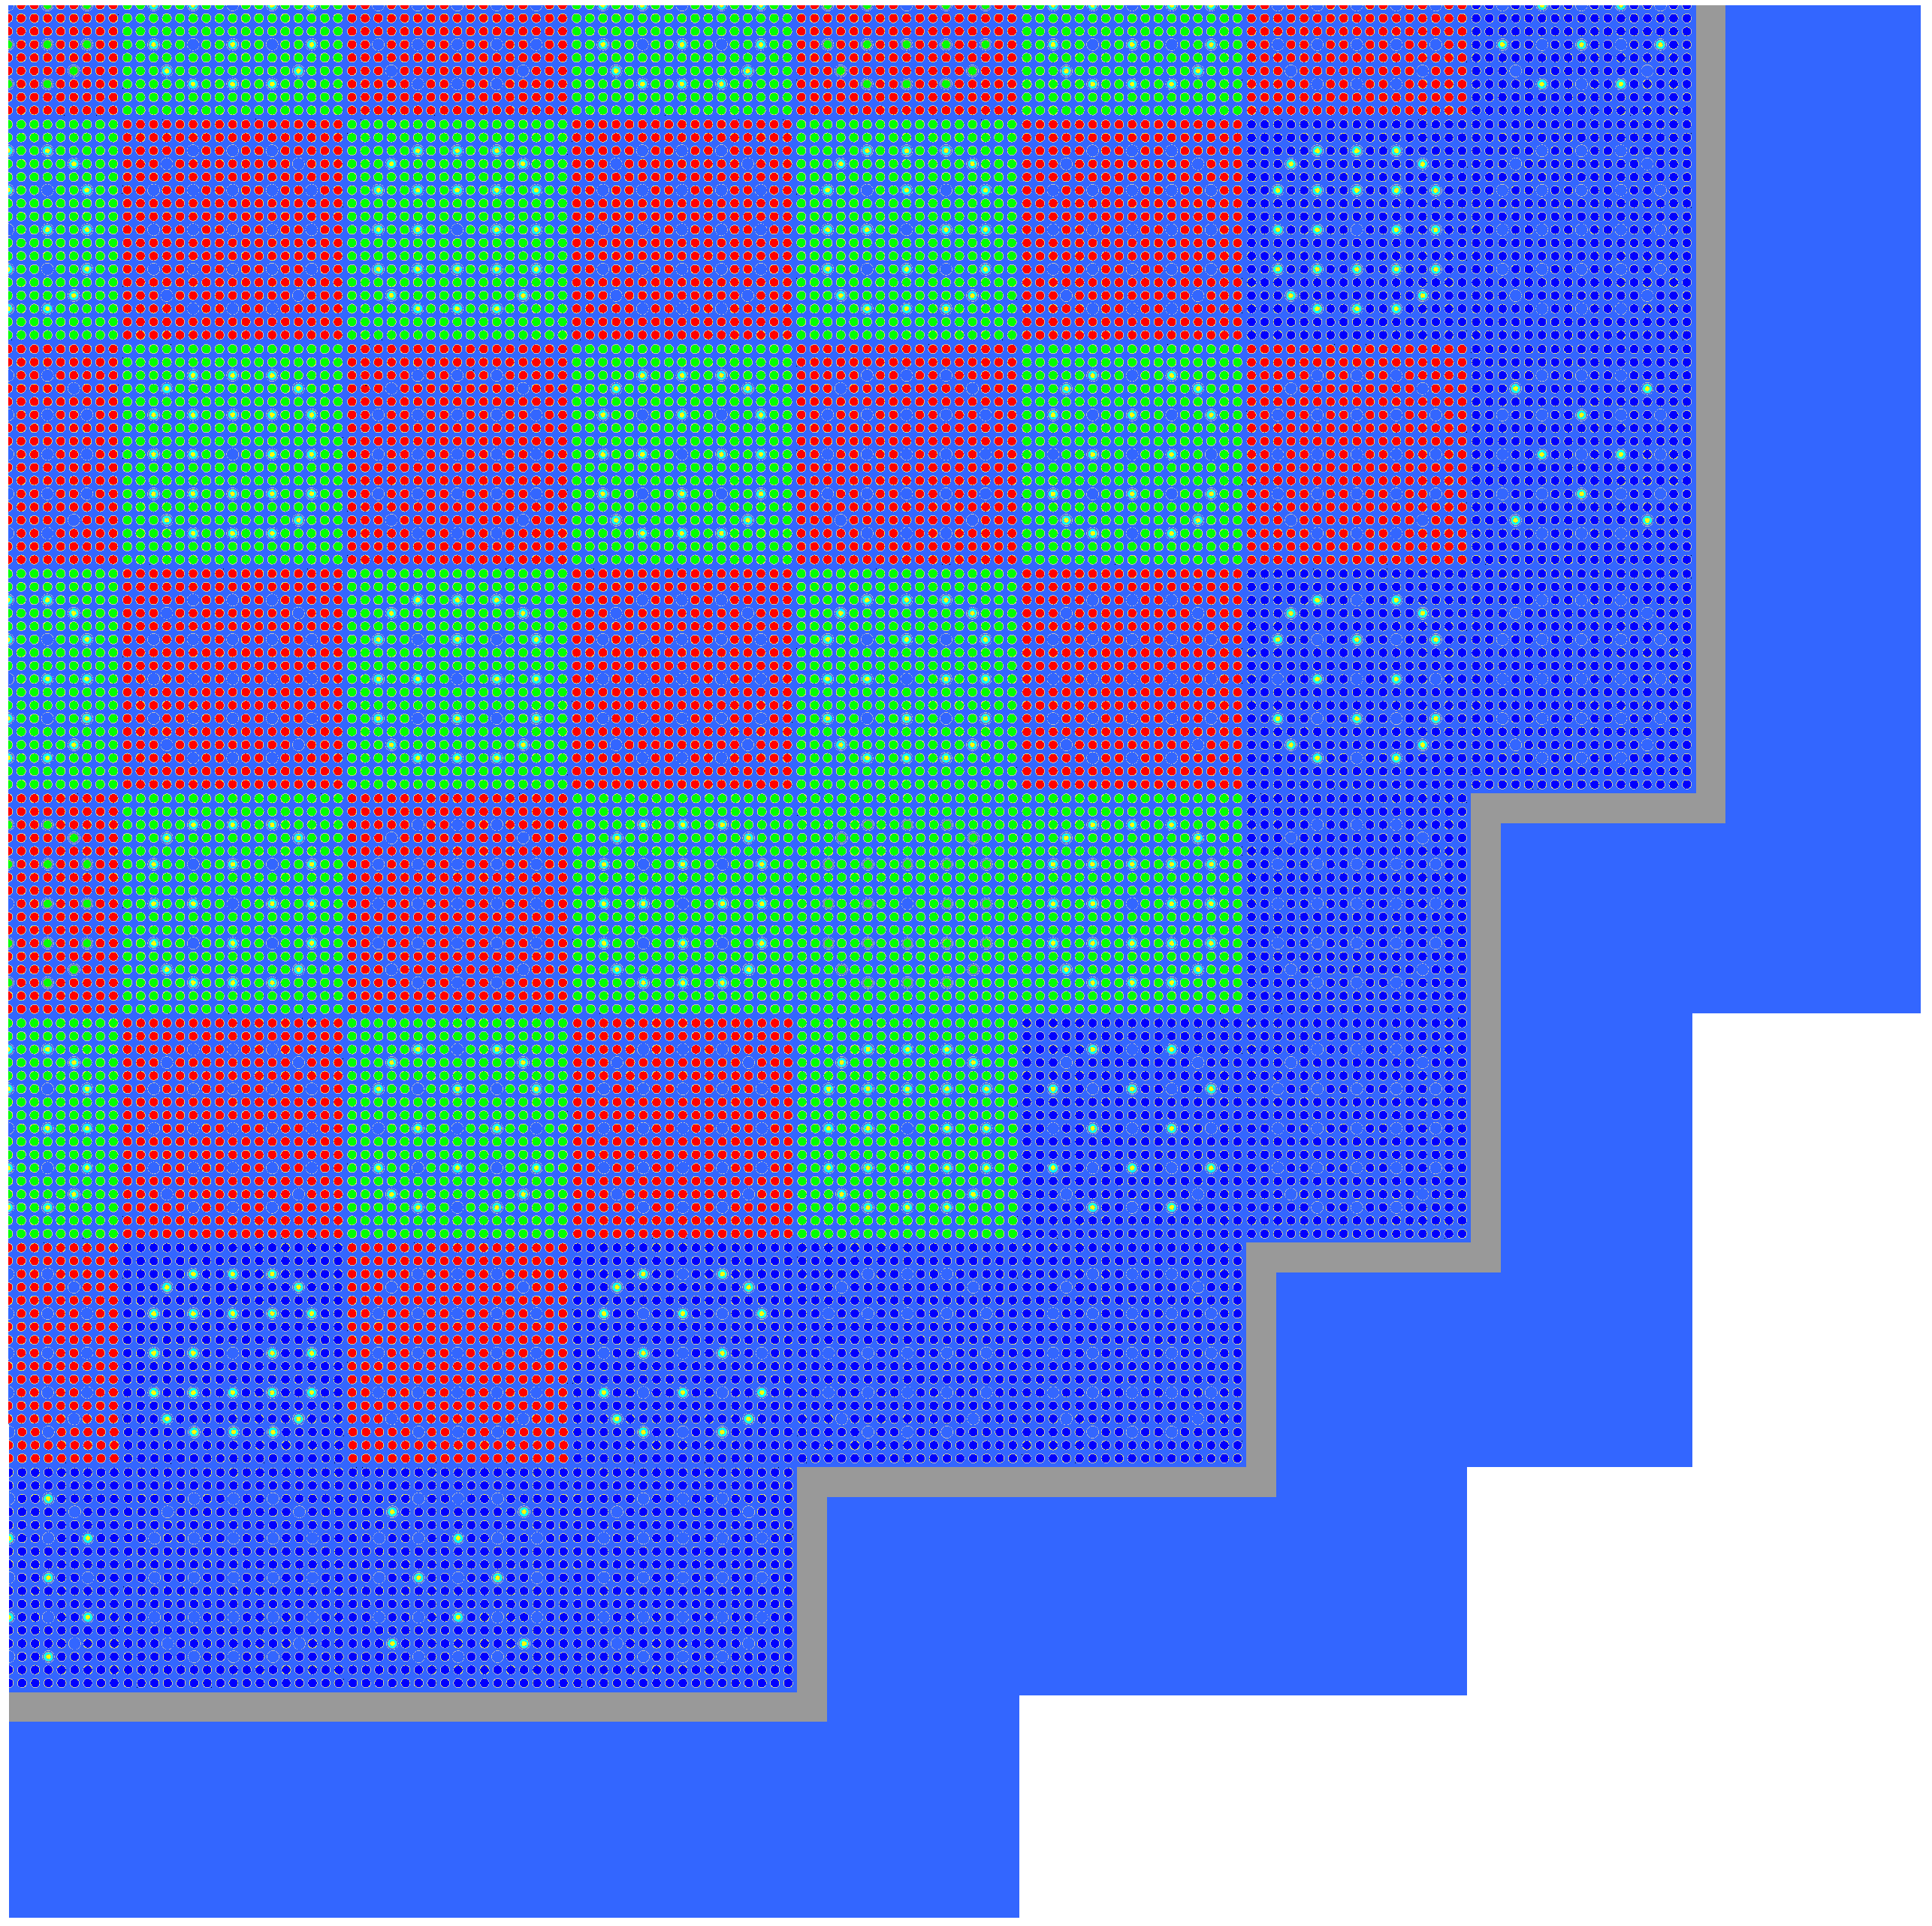
\includegraphics[width=0.48\textwidth]{p5_2D_baffle.png}
\hfill
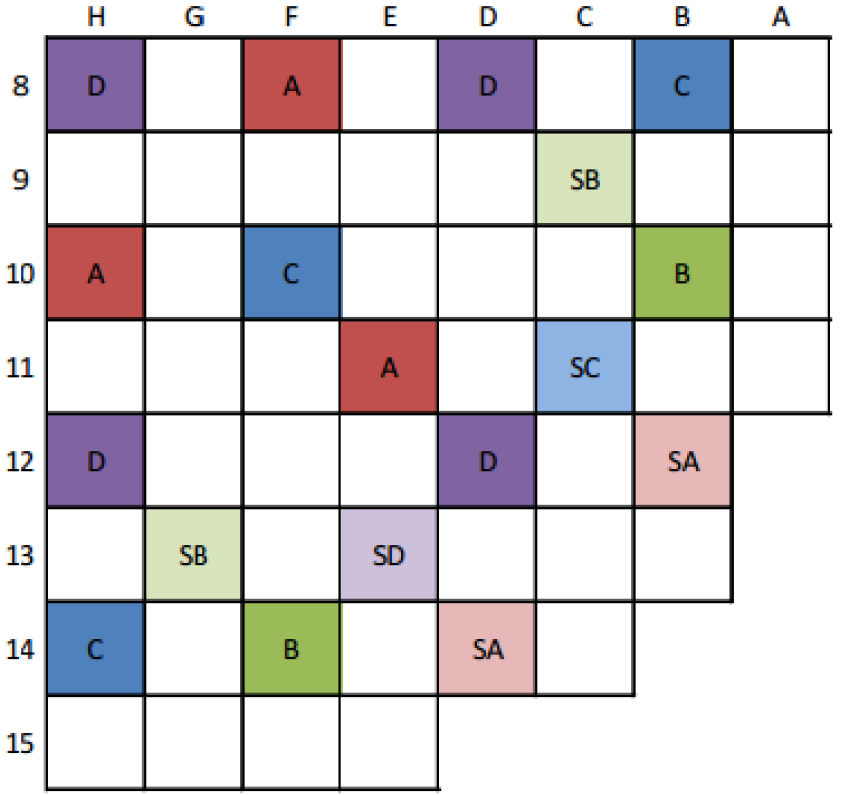
\includegraphics[width=0.48\textwidth]{WB1-cycle1-rodbank-layout.png}
\caption{VERA Problem 5 radial geometry (left) and rod bank positions (right)}\label{f:p5radial}
\end{figure}

\begin{table}[h]
\centering
\caption[VERA Problem 5 Decusping Results]{VERA Problem 5 decusping results for the partially rodded plane}\label{t:p5decusp}
\resizebox{\textwidth}{!}{
  \begin{tabular}{c c c c c c c}\toprule
    \multirow{2}{*}{Case} & \keff{} & \multicolumn{2}{|c|}{Pin Power Differences} & \multicolumn{2}{|c|}{Iterations} & Runtime\\
    & Difference (pcm) & RMS & Max & 2D/1D & CMFD & (Core-Hours) \\\midrule
    Reference        &  -- & --     & --      & 13 & 481 & 361.7 \\
    No Treatment     & -22 & 6.90\% & 30.55\% & 13 & 523 & 410.7 \\
    Polynomial       &  -5 & 1.15\% &  4.85\% & 13 & 463 & 373.7 \\
    Subplane         &  -5 & 2.09\% & 10.20\% & 13 & 499 & 399.0 \\
    Subplane + CP    &  -1 & 0.50\% &  2.74\% & 13 & 529 & 425.6 \\
    \bottomrule
  \end{tabular}
}
\end{table}

As seen in most variations of Problem 4, we see that the CP results are the best, with less than 3\% maximum error in the roded plane.  The maximum errors occur in the partially rodded assembly, as expected.  The sublpane decusping without the CP treatment is worse than in Problem 4, showing the importance of correctly treating the radial effects.  The runtime increase is also between 15\% and 20\% for the sublpane and CP decusping methods.  This is due primarily to two effects.  The first is that the convergence of the CMFD system can require more iterations using the subplane-based treatments, as discussed in the Problem 4 results.  The second effect is that there is an imbalance in the parallel partitioning of the CMFD system.  The parallel partitioning in MPACT is tied to MOC planes, so MOC planes with a larger number of subplanes will take longer to be solved than others, leaving some compute cores waiting on others to finish their calculations.  This effect would have also occurred some Problem 4, but is more significant in Problem 5 due to its larger size.  A more clever strategy for parallel decomposition would help to alleviate this imbalance and reduce the runtime of the subplane-based methods without any impact on their accuracy.

\section{C5G7 Results}

This section will focus on the results for the C5G7 benchmark problems for the subray method of characteristics.  First, 1D results generated by a simple prototype code will be presented, followed by 2D and 3D results from the 2D/1D code MPACT.  While the focus of this section is on subray MOC, the 2D and 3D results will also include the polynomial and subplane collision probabilities decusping techniques to show the accuracy of subray MOC compared with the other methods discussed already.

\subsection{1D Subray}

\begin{figure}[h]
    \centering
    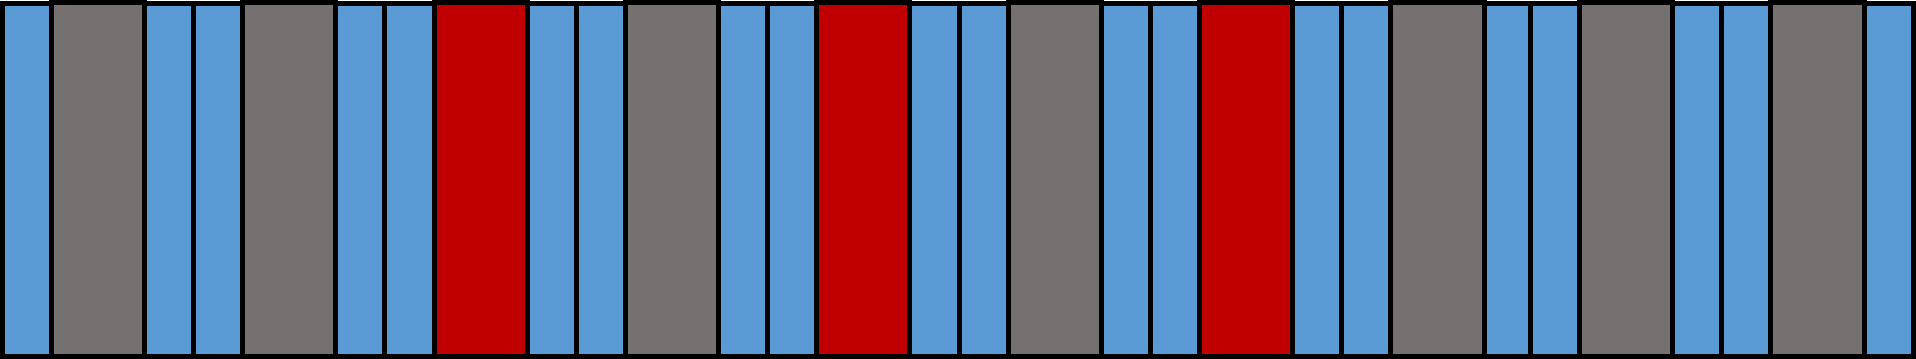
\includegraphics[width=\textwidth]{10pin-slab-geometry.png}
    \caption[Illustration of 1D MOC 10 Pin Geometry]{Illustration of 1D MOC 10 pin test geometry with materials fuel (grey), control rod/moderator mixture (red), and moderator (blue).}\label{f:10pin-geom}
\end{figure}

The 1D subray MOC results were generated using the code described in section \ref{ss:1dcode}.  To show the effectiveness of subray MOC a small 10 pin problem, illustrated in Figure \ref{f:10pin-geom}, was used.  This smaller problem was used because the rods are closer together, making it more difficult to accurately resolve the rods, and to minimize runtime.  To show the effectiveness of the subray method, a series of eigenvalue calculates was performed with the control rod volume fraction varying from 100\% to 0\% to simulate a rod withdrawal.  This was done using traditional MOC and subray MOC to show the correction achieved by using subray MOC.  The reference solution for these calculations is generated by using the volume fractions to mix the fully rodded and unrodded solutions at each iteration and calculating the updated eigenvalue.  The results of these calculations are shown in Figure \ref{f:1d-subray-keff}.

\begin{figure}[h]
    \centering
    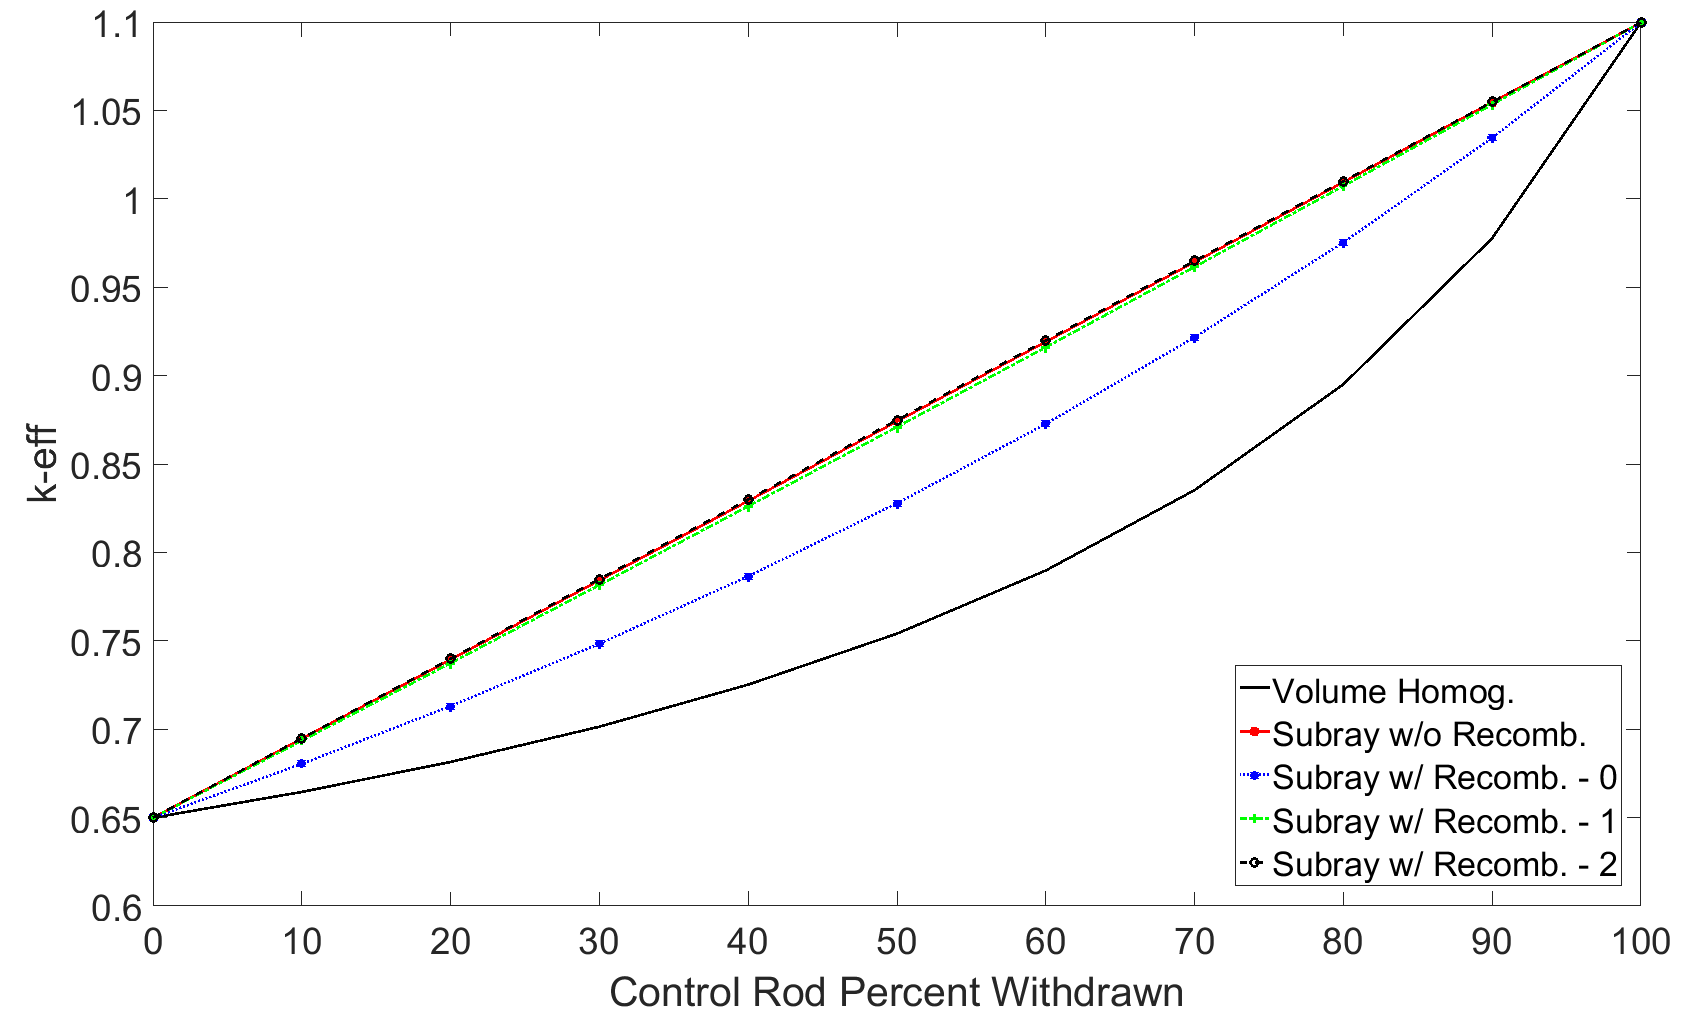
\includegraphics[width=0.8\textwidth]{keff_subray.png}
    \caption{Eigenvalue comparisons for 1D rod withdrawal}\label{f:1d-subray-keff}
\end{figure}

\begin{figure}[!htb]
    \centering
    \subfigure[Group 1]{
        \centering
        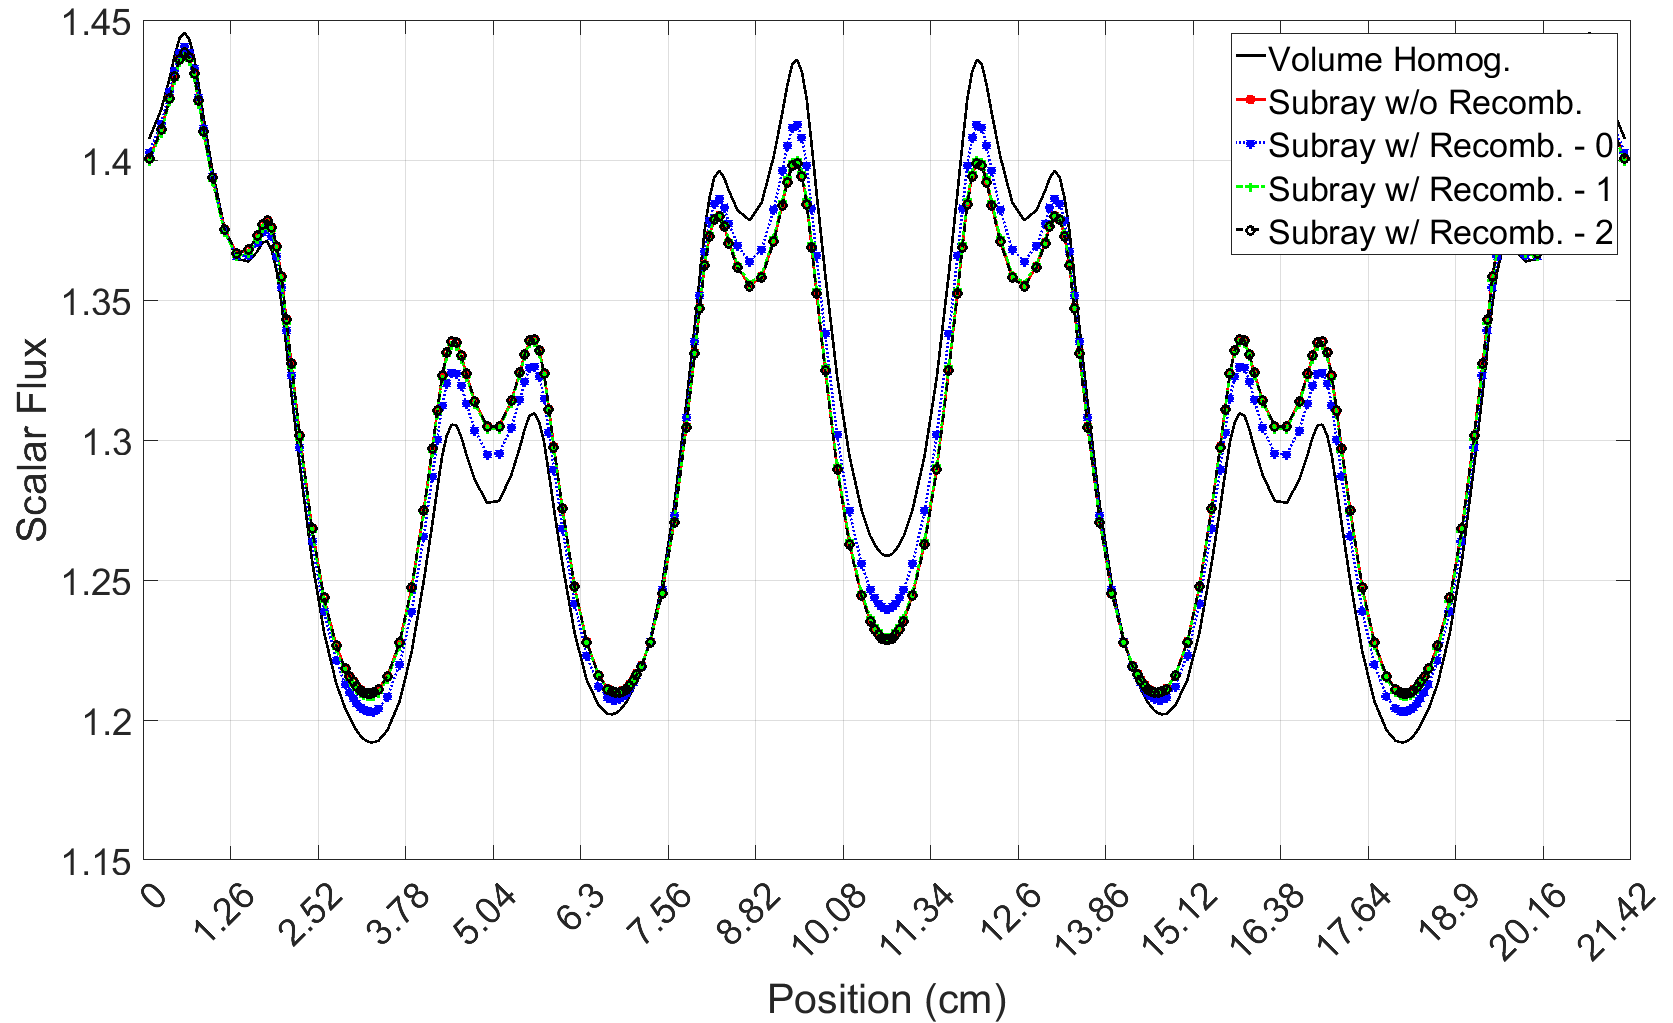
\includegraphics[width=\textwidth]{scalflux1.png}
    }
    ~
    \subfigure[Group 7]{
        \centering
        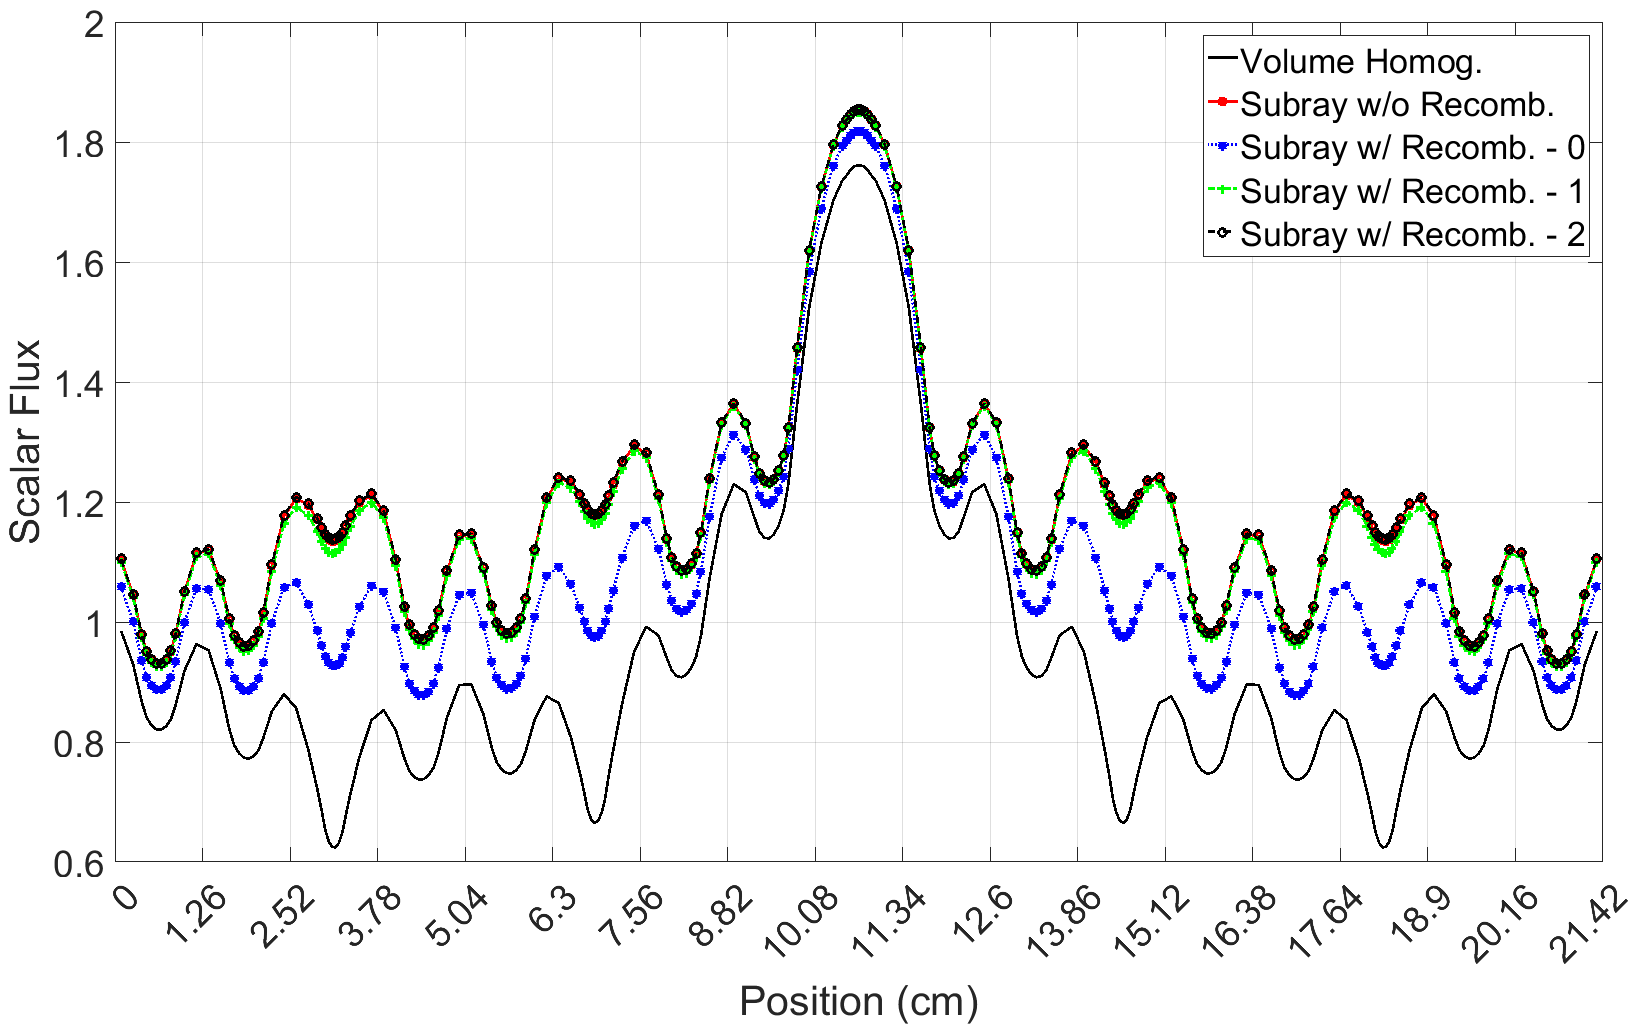
\includegraphics[width=\textwidth]{scalflux7.png}
    }
    \caption{Scalar flux distributions for 1D subray MOC calculations}\label{f:1d-subray-scalflux}
\end{figure}

In Figure \ref{f:1d-subray-keff}, the red line is subray without recombination, meaning that two completely separate solves were done each iteration and the resulting scalar fluxes were mixed using volume fractions.  The rodded and unrodded solves have separate angular flux boundary conditions which are saved for each subsequent iteration.  This provides the reference solution.  The volume homogenization solution is a traditional MOC calculation without treating the partially inserted rod.  As is evident, the errors from this method are large, nearing 15\% around 50-60\% withdrawal.  Using subray MOC in only the partially rodded pin cells, indicated in the figure by ``Subray w/ Recomb. - 0'', corrects a significant amount of the error and brings the maximum difference closer to 5\%.  Using a recombination factor of 1 means that subray is now used in all the pin cells between the control rods, correctly resolving the interference effects of the rods and eliminating almost all of the remaining error.  Finally, a recombination factor of 2 extends the subrays all the way to the problem boundary, effectively performing the same calculation as the reference solution.

In addition to the eigenvalue calculations, the scalar flux differences are shown for groups 1 and 7 at 50\% rod withdrawal in Figure \ref{f:1d-subray-scalflux}.  For both groups, it is evident that subray MOC effectively reduces the error caused by the partially inserted rod.  Only performing subray MOC in the rodded pin cells eliminates the majority of the error, but for both the eigenvalue and scalar flux distributions, it is necessary to delay recombination of the angular fluxes for at least one neighboring pin cell to capture the effects of the rod on the source in neighboring pin cells.  This effect is exaggerated by the 1D geometry since the solve is being performed exlusively in the direction that minimizes the distance between pins.  Furthermore, most PWR geometries have at least 2 pins between control rodlets, which further diminishes the effects of rod interference.  While these 1D results do not definitively indicate that recombination should be extended beyond the edge of the partially rodded pin cell, it is important to keep this in mind in the 2D and 3D calculations.

\subsection{2D C5G7}

\begin{figure}[h]
    \centering
    \subfigure{
        \centering
        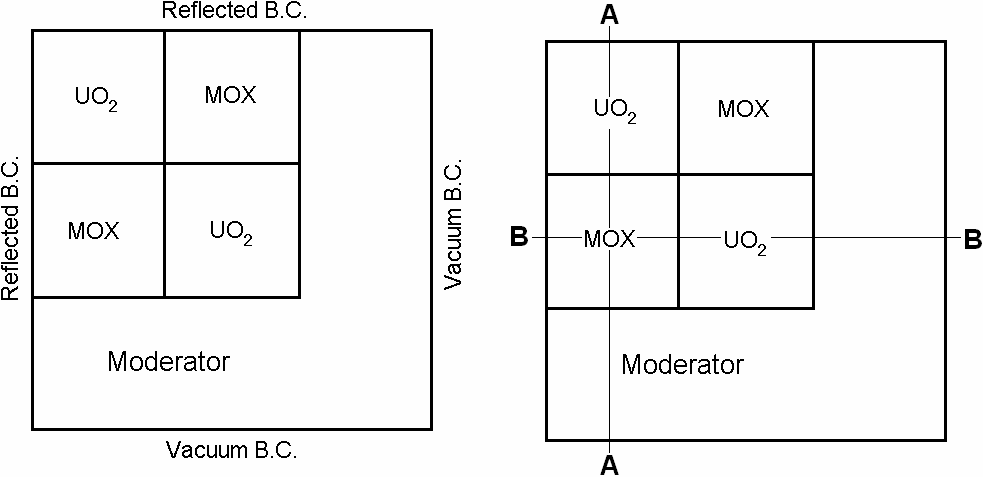
\includegraphics[width=0.8\textwidth]{c5g7-core-radial.png}
    }
    ~
    \subfigure{
        \centering
        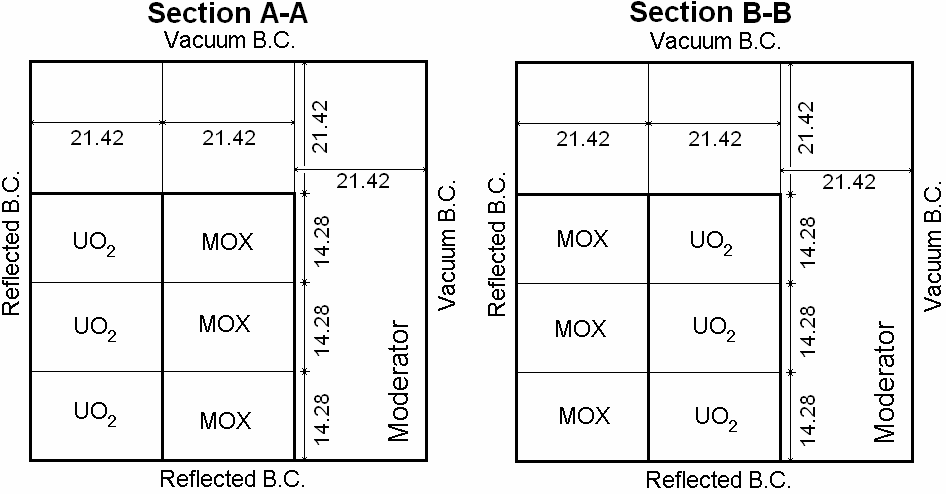
\includegraphics[width=0.8\textwidth]{c5g7-core-axial.png}
    }
    \caption{Description of C5G7 Core\cite{EELewisC5G7extended2005}}\label{f:c5g7-core}
\end{figure}

\begin{figure}[h]
    \centering
    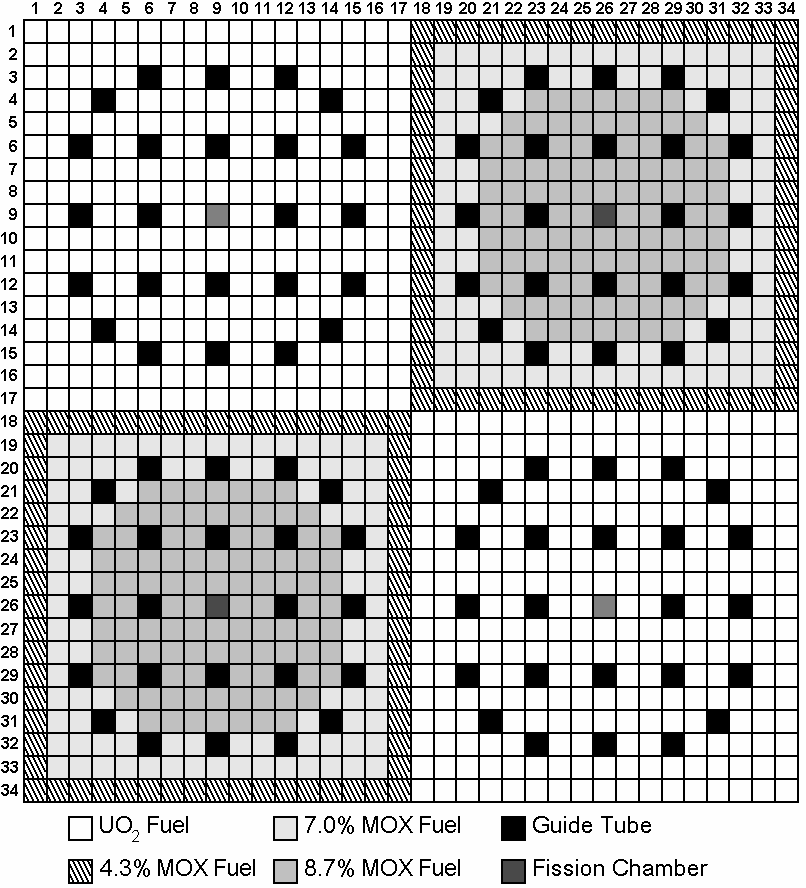
\includegraphics[width=0.8\textwidth]{c5g7-assemblies-radial.png}
    \caption{C5G7 Assembly Description\cite{EELewisC5G7extended2005}}\label{f:c5g7-assemblies}
\end{figure}

To test the mechanics of subray MOC in MPACT, 2D variations of the C5G7 benchmark problems were used.  These problems consist of 17$\times$17 UO$_2$ and MOX assemblies with control rods and a radial reflector region.  Figure \ref{f:c5g7-core} shows an illustration of the core layout, and Figure \ref{f:c5g7-assemblies} shows the assembly layout.  This section will present results for subray MOC using 3 different 2D problems derived from these descriptions.

All calculations in this section used 0.03 cm ray spacing and a Chebyshev-Yamamoto angular quadrature \hl{cite} with 16 azmiuthals and 3 polars per octant.  A 1D P$_3$ solver was used for the subplane axial calculations unless otherwise noted.  The calculations were converged until the change in both the eigenvalue and fission source were less than $10^{-6}$.  All pin meshes in the fuel assemblies used 5 radial rings in the fuel, 2 rings in the moderator, and 8 azimuthal divisions in every radial region for a total of 64 flat source regions in each pin cell.  This mesh was also used for the rodded pin cells in the axial reflector region.  The remaining axial reflector pin cells and all radial reflector pin cells used a Cartesian grid with 5 x- and y- divisions, for a total of 25 equal-volume flat source regions.

\subsubsection{UO\texorpdfstring{$_2$}{2} Assembly}

\begin{table}[h]
    \centering
    \caption{2D C5G7 UO$_2$ assembly eigenvalue and power distribution differences for subray recombination parameter sensitivity.  A * indicates that finite difference was used axially instead of P$_3$}\label{t:c5g7-2d-asy-recomb}
    \resizebox{\textwidth}{!}{
        \begin{tabular}{l c c l l c l l c l l c l l}
        \toprule
        Rod & Reference & \multicolumn{3}{c}{Subray-0} & \multicolumn{3}{c}{Subray-1} & \multicolumn{3}{c}{Subray-2} & \multicolumn{3}{c}{Subray-3} \\
        Position & \keff{} & \keff{} & \multicolumn{2}{c}{Pin Powers} & \keff{} & \multicolumn{2}{c}{Pin Powers} & \keff{} & \multicolumn{2}{c}{Pin Powers} & \keff{} & \multicolumn{2}{c}{Pin Powers} \\
        &  &  & RMS & Max &  & RMS & Max &  & RMS & Max &  & RMS & Max \\
        \midrule
1 & 1.02555  & -65  & 0.04\% & 0.08\% & -55  & 0.03\% & 0.06\% & -55  & 0.04\% & 0.11\% & -55  & 0.04\% & 0.10\% \\
2 & 1.06065  & -241 & 0.13\% & 0.27\% & -149 & 0.07\% & 0.16\% & -137 & 0.13\% & 0.37\% & -136 & 0.13\% & 0.41\% \\
3 & 1.09578  & -304 & 0.15\% & 0.31\% & -200 & 0.08\% & 0.20\% & -183 & 0.13\% & 0.38\% & -181 & 0.14\% & 0.43\% \\
4 & 1.13011  & -330 & 0.16\% & 0.31\% & -230 & 0.09\% & 0.22\% & -211 & 0.13\% & 0.36\% & -209 & 0.14\% & 0.41\% \\
5 & 1.16334  & -331 & 0.15\% & 0.29\% & -246 & 0.09\% & 0.22\% & -226 & 0.12\% & 0.31\% & -224 & 0.12\% & 0.37\% \\
6 & 1.19557  & -311 & 0.13\% & 0.26\% & -249 & 0.09\% & 0.21\% & -231 & 0.11\% & 0.26\% & -229 & 0.11\% & 0.32\% \\
7 & 1.22711  & -275 & 0.11\% & 0.22\% & -244 & 0.08\% & 0.19\% & -227 & 0.09\% & 0.21\% & -226 & 0.10\% & 0.26\% \\
8 & 1.25858  & -231 & 0.09\% & 0.17\% & -229 & 0.08\% & 0.17\% & -217 & 0.08\% & 0.17\% & -216 & 0.08\% & 0.20\% \\
        9* & 1.29513 & -66 & 0.02\% & 0.04\% & -74 & 0.02\% & 0.05\% & -74 & 0.02\% & 0.05\% & -74 & 0.03\% & 0.05\% \\
        \midrule
        Average &  -- & 239 & 0.11\% & 0.22\% & 186 & 0.07\% & 0.16\% & 173 & 0.09\% & 0.25\% & 172 & 0.10\% & 0.28\% \\
        \bottomrule
    \end{tabular}
    }
\end{table}


\begin{table}[h]
\centering
\caption{2D C5G7 UO$_2$ eigenvalue and power distribution differences for each decusping method.  A * indicates that finite difference was used axially instead of P$_3$}\label{t:c5g7-2d-asy-methods}
\resizebox{\textwidth}{!}{
    \begin{tabular}{l c c l l c l l c l l c l l}
    \toprule
    Rod & Reference & \multicolumn{3}{c}{Subray-0} & \multicolumn{3}{c}{None} & \multicolumn{3}{c}{Subplane} & \multicolumn{3}{c}{Subplane + CP} \\
    Position & \keff{} & \keff{} & \multicolumn{2}{c}{Pin Powers} & \keff{} & \multicolumn{2}{c}{Pin Powers} & \keff{} & \multicolumn{2}{c}{Pin Powers} & \keff{} & \multicolumn{2}{c}{Pin Powers} \\
    &  &  & RMS & Max &  & RMS & Max &  & RMS & Max &  & RMS & Max \\
    \midrule
1 & 1.02555  & -65  & 0.04\% & 0.08\% & -1230 & 0.70\% & 1.46\% & -370  & 0.21\% & 0.43\% & -707 & 0.35\% & 0.79\% \\
2 & 1.06065  & -241 & 0.13\% & 0.27\% & -3123 & 1.71\% & 3.55\% & -1299 & 0.70\% & 1.45\% & -626 & 0.30\% & 0.65\% \\
3 & 1.09578  & -304 & 0.15\% & 0.31\% & -4777 & 2.49\% & 5.11\% & -1645 & 0.83\% & 1.69\% & -574 & 0.26\% & 0.56\% \\
4 & 1.13011  & -330 & 0.16\% & 0.31\% & -6053 & 2.98\% & 6.09\% & -1771 & 0.83\% & 1.69\% & -522 & 0.23\% & 0.48\% \\
5 & 1.16334  & -331 & 0.15\% & 0.29\% & -6848 & 3.19\% & 6.47\% & -1745 & 0.77\% & 1.55\% & -465 & 0.20\% & 0.40\% \\
6 & 1.19557  & -311 & 0.13\% & 0.26\% & -7067 & 3.11\% & 6.26\% & -1606 & 0.66\% & 1.33\% & -400 & 0.16\% & 0.33\% \\
7 & 1.22711  & -275 & 0.11\% & 0.22\% & -6588 & 2.73\% & 5.45\% & -1375 & 0.53\% & 1.07\% & -327 & 0.13\% & 0.25\% \\
8 & 1.25858  & -231 & 0.09\% & 0.17\% & -5245 & 2.04\% & 4.03\% & -1079 & 0.39\% & 0.79\% & -242 & 0.09\% & 0.18\% \\
        9* & 1.29513 & -66 & 0.02\% & 0.04\% & -3251 & 1.17\% & 2.28\% & -445 & 0.15\% & 0.30\% & -120 & 0.04\% & 0.08\% \\
    \midrule
    Average & -- & 239 & 0.11\% & 0.22\% & 4909 & 2.24\% & 4.52\% & 1259 & 0.56\% & 1.14\% & 443 & 0.20\% & 0.41\% \\
    \bottomrule
    \end{tabular}
}
\end{table}

The first 2D problem is a single UO$_2$ assembly with control rods added to it.  A similar procedure was followed as with the 1D calculations with the problem being simulated at 10\% increments during the rod withdrawal.  The reference for these calculations was generated by dividing the MOC plane into two separate planes with their boundary aligned with the control rod.  Comparisons could then be made between the decusping methods and the reference solution for \keff{} and the radial power distribution.

Table \ref{t:c5g7-2d-asy-recomb} shows the results for the 2D assembly case for recombination factor values of 0, 1, 2, and 3.  The \keff{} differences trend toward 0 as the recombination factor is increased.  This is to be expected since using subray MOC in a larger number of regions surrounding the control rodlets should increase the resolution of the axial shape of the solution.  However, for the single assembly case, the \keff{} differences are still large even for the Subray-3 calculations.  The power distribution differences show a different trend.  The Subray-1 option improves significantly on the Subray-0 option for both RMS and maximum power differences.  However, the Subray-2 and Subray-3 calculations are both worse than Subray-1 and give solutions comparable to the Subray-0 option.

Table \ref{t:c5g7-2d-asy-methods} compares the results of subray MOC with the sublpane-based decusping methods described earlier.  The polynomial method is not compared because the data required to use them fo C5G7 has not been generated.  The subplane decusping method performs better with CP than without, as expected.  Overall, its performance is good, reducing the maximum power error to around 0.5\% on average and reducing the \keff{} error from an average of almost 5\% to under 500 pcm.  However, the Subray-0 treatment performs better than the Subplane + CP method, reducing the maximum power error to less than 0.3\% for almost every case.  The \keff{} error is also reduced to an average of -239 pcm.

This relationship between Subplane + CP and Subray-0 is expected.  Both of them are improving the solution in a single pin cell by solving the rodded and unrodded levels separately.  However, Subplane + CP does this after the MOC calculation, improving only the CMFD and 1D P$_3$ cross sections.  The Subray-0 calculation uses 2D MOC, which should provide a solution superior to 1D CP.  It also calculates improved radial currents, and improves the solution in pins neighboring the control rodlets by improving the angular flux exiting the control rod pin cells.  Thus, it is expected that Subray-0 would consistently provide a better solution than the Subplane + CP decusing method.

It should be noted at this point that certain calculations whose results are shown in these and following tables failed to converge using the axial P$_3$ solver.  This occurred for all calculations that had multiple planes or used the subplane scheme.  This is a known issue with the axial solvers caused by the interpolation of the radial TL source.  Whenever a thin plane is next to a thick plane and a very large change in the radial TL occurs from the thin plane to the thick plane, the quadratic interpolation of the radial TL can cause shapes that make the P$_3$ solver unstable.  This can be shown to be the source of the instability by limiting the magnitude of the linear and quadratic components of the shape.

One of the other MPACT developers is currently implementing a new solver that employs a different technique to solve the P$_3$ equations, and is expected to resolve this instability.  Since that solver is not yet ready for use and limiting the linear and/or quadratic moments of the radial TL interpolation can have significant effects on accuracy, the cases which did not converge for either the reference or decusping method calculations simply used the axial currents from the CMFD calculation with no 1D axial solver.  While the actual accuracy of the calculations is worse when using finite difference, the behavior is predictable and allows for consistent comparisons of the subray MOC with multi-plane calculations.  The results that used finite difference instead of P$_3$ will be denoted with an asterisk (*) in all tables in this section.

\begin{table}[h]
    \centering
    \caption{Long Ray Data for 2D C5G7 UO\texorpdfstring{$_2$}{2} Rodded Assembly}\label{t:subray-data-2dassembly}
    \begin{tabular}{l l l}\toprule
        Method & Long Rays per Plane & Increase \\\midrule
        Reference & 29480 & -- \\
        Subray-0 & 48440 & 64\% \\
        Subray-1 & 52832 & 79\% \\
        Subray-2 & 56304 & 91\% \\
        Subray-3 & 58960 & 100\% \\
        \bottomrule
    \end{tabular}
\end{table}

\begin{table}[h]
    \centering
    \caption{Average Performance and Convergence Data for C5G7 Rodded UO\texorpdfstring{$_2$}{2} Assembly}\label{t:subray-performance-2dassembly}
    \begin{tabular}{l l l l}\toprule
        Method & Iterations & Runtime (s) & Speedup \\\midrule
Reference     & 16.4 & 119 & --   \\
None          & 14.6 & 56 & 2.14 \\
Subplane      & 14.9 & 57 & 2.10 \\
Subplane + CP & 15.2 & 63 & 1.91 \\
Subray-0      & 14.9 & 94 & 1.27  \\
Subray-1      & 15.3 & 104 & 1.15 \\ 
Subray-2      & 15.4 & 109 & 1.09 \\ 
Subray-3      & 15.3 & 107 & 1.11 \\ 
        \bottomrule
    \end{tabular}
\end{table}

While the subray MOC method is more accurate than the previous decusping methods, it is also more expensive.  Table \ref{t:subray-data-2dassembly} shows the long ray data for the reference case and each variation of the subray MOC calculations.  The first column is the total number of long rays including those duplicated for subray MOC.  The second column shows the percent increase in the number of long rays.  This value can be used to approximate the savings obtained by using subray MOC to resolve partially inserted rods instead of 2 separate MOC planes.  For the single assembly case, it is expected that Subray-3 and the reference case would take about the same amount of time for each MOC sweep since every long ray was duplicated for Subray-3.

Table \ref{t:subray-performance-2dassembly} shows the convergence and runtime data for each decusping method averaged over all 9 rod positions. The speedup of each case is defined as the reference runtime divided by the comparison runtime.  Using Table \ref{t:subray-data-2dassembly}, we can approximate an expected speedup for each case by taking the number of long rays in the reference (2 MOC planes) and dividing by the number in the comparison case (1 MOC plane).  Doing this, we get expected speedups of 1.22, 1.12, 1.05, and 1.0 for Subray-0, Subray-1, Subray-2, and Subray-3, respectively.  The observed speedups are similar to, but consistently a little better than predicted.  Subray MOC takes between 1 and 1.5 iterations fewer, on average, than the reference case.  Furthermore, there is some small gain in efficiency from having all the long rays in a single sweep instead of two separate sweeps, though this is a smaller effect.  Thus, subray MOC performs about as well as expected for this implementation.  The other methods all see a speedup around 2.0, which is expected since the amount of time spent in MOC is exactly half that of the reference.  The differences in the CMFD solve and number of iterations introduce some variation in the speedup, which is to be expected.

\subsubsection{2D Core -- Rodded Center Assembly}

\begin{table}[h]
    \centering
    \caption{2D C5G7 center assembly rod withdrawal eigenvalue and pin power differences for subray recombination parameter sensitivity.  A * indicates that finite difference was used axially instead of P$_3$}\label{t:c5g7-2d-center-recomb}
    \resizebox{\textwidth}{!}{
        \begin{tabular}{l c c l l c l l c l l c l l}
            \toprule
            Rod & Reference & \multicolumn{3}{c}{Subray-0} & \multicolumn{3}{c}{Subray-1} & \multicolumn{3}{c}{Subray-2} & \multicolumn{3}{c}{Subray-3} \\
            Position & \keff{} & \keff{} & \multicolumn{2}{c}{Pin Powers} & \keff{} & \multicolumn{2}{c}{Pin Powers} & \keff{} & \multicolumn{2}{c}{Pin Powers} & \keff{} & \multicolumn{2}{c}{Pin Powers} \\
            &  &  & RMS & Max &  & RMS & Max &  & RMS & Max &  & RMS & Max \\
            \midrule
            1* & 1.06846 & -16 & 0.09\% & 0.24\% & -13 & 0.08\% & 0.20\% & -13 & 0.07\% & 0.18\% & -13 & 0.07\% & 0.18\% \\
2 & 1.07746 & -65  & 0.37\% & 1.03\% & -38  & 0.22\% & 0.60\% & -35  & 0.18\% & 0.47\% & -34  & 0.17\% & 0.46\% \\
3 & 1.08597 & 87   & 0.50\% & 1.46\% & 121  & 0.32\% & 0.91\% & 128  & 0.26\% & 0.73\% & 128  & 0.26\% & 0.72\% \\
4 & 1.09919 & -114 & 0.58\% & 1.77\% & -76  & 0.39\% & 1.15\% & -68  & 0.33\% & 0.96\% & -67  & 0.32\% & 0.95\% \\
5 & 1.11160 & -127 & 0.61\% & 1.92\% & -91  & 0.44\% & 1.34\% & -81  & 0.37\% & 1.14\% & -80  & 0.36\% & 1.13\% \\
6 & 1.12495 & -132 & 0.59\% & 1.92\% & -103 & 0.46\% & 1.45\% & -92  & 0.40\% & 1.26\% & -91  & 0.39\% & 1.25\% \\
7 & 1.13925 & -128 & 0.53\% & 1.78\% & -110 & 0.46\% & 1.48\% & -100 & 0.41\% & 1.33\% & -99  & 0.40\% & 1.32\% \\
8 & 1.15469 & -117 & 0.45\% & 1.53\% & -113 & 0.44\% & 1.45\% & -105 & 0.40\% & 1.34\% & -104 & 0.39\% & 1.33\% \\
            9* & 1.17431 & -36  & 0.13\% & 0.44\% & -40  & 0.14\% & 0.46\% & -40  & 0.14\% & 0.46\% & -40  & 0.14\% & 0.46\% \\
            \midrule
            Average & -- & 91 & 0.43\% & 1.34\% & 78 & 0.33\% & 1.00\% & 73 & 0.28\% & 0.88\% & 73 & 0.28\% & 0.87\% \\
            \bottomrule
        \end{tabular}
    }
\end{table}

\begin{table}[h]
    \centering
    \caption{2D C5G7 center assembly rod withdrawal eigenvalue and pin power differences for each decusping method.  A * indicates that finite difference was used axially instead of P$_3$}\label{t:c5g7-2d-center-methods}
    \resizebox{\textwidth}{!}{
        \begin{tabular}{l c c l l c l l c l l c l l}
            \toprule
            Rod & Reference & \multicolumn{3}{c}{Subray-0} & \multicolumn{3}{c}{None} & \multicolumn{3}{c}{Subplane} & \multicolumn{3}{c}{Subplane + CP} \\
            Position & \keff{} & \keff{} & \multicolumn{2}{c}{Pin Powers} & \keff{} & \multicolumn{2}{c}{Pin Powers} & \keff{} & \multicolumn{2}{c}{Pin Powers} & \keff{} & \multicolumn{2}{c}{Pin Powers} \\
            &  &  & RMS & Max &  & RMS & Max &  & RMS & Max &  & RMS & Max \\
            \midrule
            1* & 1.06846 & -16 & 0.09\% & 0.24\% & -294 & 1.76\% & 4.53\% & -90 & 0.53\% & 1.38\% & -171 & 1.01\% & 2.50\% \\
2 & 1.07746 & -65  & 0.37\% & 1.03\% & -811  & 4.75 \% & 12.70\% & -348 & 2.01\% & 5.46\% & -174 & 0.97\% & 2.57\% \\
3 & 1.08597 & 87   & 0.50\% & 1.46\% & -1189 & 7.71 \% & 21.30\% & -318 & 2.73\% & 7.70\% & -1   & 0.97\% & 2.70\% \\
4 & 1.09919 & -114 & 0.58\% & 1.77\% & -1918 & 10.33\% & 29.42\% & -603 & 3.12\% & 9.12\% & -185 & 0.94\% & 2.75\% \\
5 & 1.11160 & -127 & 0.61\% & 1.92\% & -2400 & 12.25\% & 36.00\% & -663 & 3.21\% & 9.72\% & -184 & 0.88\% & 2.68\% \\
6 & 1.12495 & -132 & 0.59\% & 1.92\% & -2738 & 13.12\% & 39.83\% & -674 & 3.04\% & 9.49\% & -174 & 0.78\% & 2.47\% \\
7 & 1.13925 & -128 & 0.53\% & 1.78\% & -2820 & 12.55\% & 39.38\% & -631 & 2.64\% & 8.48\% & -155 & 0.65\% & 2.11\% \\
8 & 1.15469 & -117 & 0.45\% & 1.53\% & -2478 & 10.08\% & 32.80\% & -535 & 2.06\% & 6.83\% & -124 & 0.48\% & 1.62\% \\
            9* & 1.17431 & -36  & 0.13\% & 0.44\% & -1702 & 6.13\% & 20.82\% & -239 & 0.83\% & 2.81\% & -65  & 0.23\% & 0.79\% \\
            \midrule
            Average & -- & 91 & 0.43\% & 1.34\% & 1817 & 8.74\% & 26.31\% & 456 & 2.24\% & 6.78\% & 137 & 0.77\% & 2.24\% \\
            \bottomrule
        \end{tabular}
    }
\end{table}

The second problem uses the full radial core layout from Figures \ref{f:c5g7-core} and \ref{f:c5g7-assemblies}.  A control rod was added to the northwest UO$_2$ assembly, and the same procedure was followed as for the 2D assembly.  Table \ref{t:c5g7-2d-center-recomb} shows the results for subray MOC as a function of recombination value.  The trends observed in these results match more closely with expectations.  As the recombination factor is increased from 0 to 3, the errors monotically decrease.  The largest jump occurs from Subray-0 to Subray-1, and the smallest from Subray-2 to Subray-3.  This matches both physical intuition about the local effects of each control rodlet as well as the results of the 1D prototype subray MOC calculations.  The decrease in error from Subray-2 to Subray-3 might be slightly larger if the recombination were not restricted to the rodded assembly, as described by Figure \ref{f:recombination}.  However, the additional benefits from Subray-3 are likely insignificant when compared with the time to implement that logic and increased runtime of subray MOC.

Table \ref{t:c5g7-2d-center-methods} compares subray MOC to the other methods. The same observations can be made for these calculations as for the 2D assembly calculations.  The subplaned decusping is much better with CP than without, and subray MOC is better still, reducing the maximum power differences from around 25\% to less than 2\% for every rod position.  Furthermore, the \keff{} differences are reduced from almost around 2\% with no treatment and around 150 pcm with Subplane + CP to less than 100 pcm on average with Subray-0.

\begin{table}[h]
    \centering
    \caption{Long Ray Data for C5G7 Core}\label{t:subray-data-2dcore}
    \begin{tabular}{l l l }\toprule
        Method & Long Rays per Plane & Increase \\\midrule
        Reference & 88440 & -- \\
        Subray-0 & 107400 & 21\% \\
        Subray-1 & 111792 & 26\% \\
        Subray-2 & 115264 & 30\% \\
        Subray-3 & 117920 & 33\% \\
        \bottomrule
    \end{tabular}
\end{table}

\begin{table}[h]
    \centering
    \caption{Average Performance and Convergence Data for 2D C5G7 Core with Rodded NW Assembly}\label{t:subray-performance-2dcoreNW}
    \begin{tabular}{l l l l}\toprule
        Method & Iterations & Runtime (s) & Speedup \\\midrule
Reference     & 25.7 & 1107 & --  \\
None          & 25.8 & 739 & 1.50 \\ 
Subplane      & 26.7 & 725 & 1.53 \\ 
Subplane + CP & 26.9 & 695 & 1.61 \\
Subray-0      & 26.4 & 861 & 1.29 \\ 
Subray-1      & 25.9 & 881 & 1.26 \\ 
Subray-2      & 26.1 & 920 & 1.21 \\ 
Subray-3      & 26.1 & 938 & 1.18 \\ 
        \bottomrule
    \end{tabular}
\end{table}

As with the single assembly, the long ray data can again be used to make some predictions about performance.  Because this problem has multiple assemblies and only one is partially rodded, the speedup observed for subray MOC is expected to be larger than that of the single assembly case.  Using the same procedure as for the assembly, we can predict approximate speedups of 1.65, 1.59, 1.54, and 1.50 for Subray-0, Subray-1, Subray-2, and Subray-3, respectively.  In this case the observed speedups are significantly worse than predicted, for several reasons.  First, subray MOC takes more iterations on average than the reference.  Second, the subplane CMFD and P$_3$ systems are the same size for all decusping methods as for the reference.  This was not important for the single assembly, but the 2D core is large enough that these other parts of the 2D/1D iteration can no longer be ignored in predicting the runtime.  However, in spite of these issues, a speedup of 20-30\% is still achieved with each of the subray MOC methods.

\subsubsection{2D Core -- Rodded Corner Assembly}

\begin{table}[h]
    \centering
    \caption{2D C5G7 corner assembly rod withdrawal eigenvalue and pin power differences for subray recombination parameter sensitivity.  A * indicates that finite difference was used axially instead of P$_3$}\label{t:c5g7-2d-corner-recomb}
    \resizebox{\textwidth}{!}{
        \begin{tabular}{l c c l l c l l c l l c l l}
            \toprule
            Rod & Reference & \multicolumn{3}{c}{Subray-0} & \multicolumn{3}{c}{Subray-1} & \multicolumn{3}{c}{Subray-2} & \multicolumn{3}{c}{Subray-3} \\
            Position & \keff{} & \keff{} & \multicolumn{2}{c}{Pin Powers} & \keff{} & \multicolumn{2}{c}{Pin Powers} & \keff{} & \multicolumn{2}{c}{Pin Powers} & \keff{} & \multicolumn{2}{c}{Pin Powers} \\
            &  &  & RMS & Max &  & RMS & Max &  & RMS & Max &  & RMS & Max \\
            \midrule
            1* & 1.18889 & -2   & 0.02\% & 0.08\% & -1   & 0.02\% & 0.06\% & -1   & 0.02\% & 0.06\% & -1 & 0.02\% & 0.06\% \\
2 & 1.18966 & -6  & 0.09\% & 0.28\%  & -4 & 0.05\% & 0.14\% & -3 & 0.05\% & 0.13\% & -3 & 0.04\% & 0.13\% \\
3 & 1.19048 & -9  & 0.12\% & 0.37\%  & -5 & 0.07\% & 0.20\% & -5 & 0.06\% & 0.18\% & -4 & 0.06\% & 0.18\% \\
4 & 1.19135 & -10 & 0.14\% & 0.43\%  & -6 & 0.09\% & 0.24\% & -5 & 0.08\% & 0.22\% & -5 & 0.08\% & 0.22\% \\
5 & 1.19227 & -11 & 0.15\% & 0.46\%  & -7 & 0.11\% & 0.28\% & -6 & 0.09\% & 0.26\% & -6 & 0.09\% & 0.25\% \\
6 & 1.19324 & -11 & 0.16\% & 0.46\%  & -8 & 0.12\% & 0.31\% & -7 & 0.10\% & 0.28\% & -7 & 0.10\% & 0.28\% \\
7 & 1.19427 & -11 & 0.15\% & 0.43\%  & -9 & 0.12\% & 0.33\% & -8 & 0.11\% & 0.30\% & -8 & 0.11\% & 0.30\% \\
8 & 1.19538 & -10 & 0.14\% & 0.38\%  & -9 & 0.13\% & 0.34\% & -8 & 0.12\% & 0.32\% & -8 & 0.12\% & 0.32\% \\
            9* & 1.19684 & -3   & 0.04\% & 0.12\% & -3   & 0.05\% & 0.12\% & -3   & 0.05\% & 0.12\% & -3   & 0.05\% & 0.12\% \\
            \midrule
            Average & -- & 8 & 0.11\% & 0.33\% & 6 & 0.08\% & 0.22\% & 5 & 0.08\% & 0.21\% & 5 & 0.07\% & 0.21\% \\
            \bottomrule
        \end{tabular}
    }
\end{table}

\begin{table}[h]
    \centering
    \caption{2D C5G7 corner assembly rod withdrawal eigenvalue and pin power differences for each decusping method.  A * indicates that finite difference was used axially instead of P$_3$}\label{t:c5g7-2d-corner-methods}
    \resizebox{\textwidth}{!}{
        \begin{tabular}{l c c l l c l l c l l c l l}
            \toprule
            Rod & Reference & \multicolumn{3}{c}{Subray-0} & \multicolumn{3}{c}{None} & \multicolumn{3}{c}{Subplane} & \multicolumn{3}{c}{Subplane + CP} \\
            Position & \keff{} & \keff{} & \multicolumn{2}{c}{Pin Powers} & \keff{} & \multicolumn{2}{c}{Pin Powers} & \keff{} & \multicolumn{2}{c}{Pin Powers} & \keff{} & \multicolumn{2}{c}{Pin Powers} \\
            &  &  & RMS & Max &  & RMS & Max &  & RMS & Max &  & RMS & Max \\
            \midrule
            1* & 1.18889 & -2   & 0.02\% & 0.08\% & -27  & 0.44\% & 1.39\% & -8   & 0.13\% & 0.43\% & -16  & 0.25\% & 0.74\% \\
2 & 1.18966 & -6  & 0.09\% & 0.28\% & -71  & 1.16\% & 3.57\% & -31 & 0.49\% & 1.52\% & -16 & 0.24\% & 0.74\% \\
3 & 1.19048 & -9  & 0.12\% & 0.37\% & -114 & 1.86\% & 5.67\% & -42 & 0.66\% & 2.01\% & -16 & 0.24\% & 0.74\% \\
4 & 1.19135 & -10 & 0.14\% & 0.43\% & -153 & 2.50\% & 7.48\% & -48 & 0.76\% & 2.27\% & -17 & 0.24\% & 0.73\% \\
5 & 1.19227 & -11 & 0.15\% & 0.46\% & -185 & 3.01\% & 8.84\% & -52 & 0.81\% & 2.35\% & -16 & 0.23\% & 0.70\% \\
6 & 1.19324 & -11 & 0.16\% & 0.46\% & -205 & 3.32\% & 9.58\% & -52 & 0.80\% & 2.28\% & -15 & 0.22\% & 0.64\% \\
7 & 1.19427 & -11 & 0.15\% & 0.43\% & -207 & 3.33\% & 9.43\% & -48 & 0.74\% & 2.05\% & -13 & 0.19\% & 0.55\% \\
8 & 1.19538 & -10 & 0.14\% & 0.38\% & -182 & 2.89\% & 7.98\% & -41 & 0.63\% & 1.70\% & -11 & 0.15\% & 0.43\% \\
            9* & 1.19684 & -3   & 0.04\% & 0.12\% & -128  & 2.00\% & 5.41\% & -19   & 0.28\% & 0.74\% & -5   & 0.08\% & 0.21\% \\
            \midrule
            Average & -- & 8 & 0.11\% & 0.33\% & 141 & 2.28\% & 6.59\% & 38 & 0.59\% & 1.70\% & 14 & 0.20\% & 0.61\% \\
            \bottomrule
        \end{tabular}
    }
\end{table}

The final 2D problem is the same as the previous one, except that the southeast corner UO$_2$ assembly is rodded instead of the northwest assembly.  Tables \ref{t:c5g7-2d-corner-recomb} and \ref{t:c5g7-2d-corner-methods} show similar results to the previous two problems.  For all methods, the errors are lower for this problem than for the first multi-assembly problem.  There are two reasons for this.  First, the control rods for this problem are in a lower power region than for the previous one, so the absolute differences in power are sure to be smaller for any decusping method.  Second, the rodded assembly is not next to reflecting boundary conditions.  In the previous problem, if the reflecting boundary conditions are accounted for, there are effectively 4 rodded assemblies in a cluster in the center of the core.  However, all subrays are forced to recombine at the problem boundary, a decision which is not necessary but was made for the sake of code simplicity and time.  This likely has at least some negative impact on the results of the previous problem.  The rodded assembly in this problem is surrounded by unrodded assemblies that do not require subray MOC, removing one approximation that was forced by the other problem.

\begin{table}[h]
    \centering
    \caption{Average Performance and Convergence Data for 2D C5G7 Core with Rodded SE Assembly}\label{t:subray-performance-2dcoreSE}
    \begin{tabular}{l l l l}\toprule
        Method & Iterations & Runtime (s) & Speedup \\\midrule
Reference     & 24.4 & 1006 &     \\
None          & 24.0 & 657 & 1.54 \\
Subplane      & 25.3 & 636 & 1.59 \\
Subplane + CP & 25.3 & 629 & 1.60 \\
Subray-0      & 25.3 & 798 & 1.26 \\
Subray-1      & 25.0 & 833 & 1.21 \\
Subray-2      & 25.0 & 855 & 1.18 \\
Subray-3      & 25.0 & 878 & 1.15 \\
        \bottomrule
    \end{tabular}
\end{table}

The primary reason to show this problem is that because the rods are in the center of the model, the long rays duplicated for the subray MOC calculation are longer for some angles, especially those between the northeast and southwest corners of the model.  Thus, while the total number of rays duplicated is the same as for the previous problem (Table \ref{t:subray-data-2dcore}), the amount of work done for the duplicated rays is different.  This will show what, if any, impact the position of the control rods in the core could have on the efficiency of the subray MOC calculations.

Table \ref{t:subray-performance-2dcoreSE} shows the convergence and runtime data for this problem.  Compared with the previous 2D core problem, the speedups are similar, but lower by about 0.03 for each subray MOC calculation.  The convergence behavior of this problem is similar to the previous one, so this small decrease in speedup is likely due to duplicating longer core rays.  Overall, the impact of the control rod locations has a negligible impact on the speedups observed by using subray MOC or the other decusping methods.

\subsection{3D C5G7 UO\texorpdfstring{$_2$}{2} Assembly}

One 3D problem was also used to test subray MOC.  This problem consists of the NW UO$_2$ assembly.  As shown in figure \ref{f:c5g7-core}, this assembly has a 42.84 cm active fuel height with a 21.42 cm axial reflector on top.  The control rods at full insertion extend from the bottom of the active fuel all the way to the top of the reflector.  In MPACT, this was modeled using 4 MOC planes: 3 in the active fuel region and 1 for the axial refelctor.  The rod was withdrawn from the bottom of the fuel to the top in 30 steps of 1.428 cm.  At each position, a reference solution was generated using the same method as the 2D calculations by adding an extra MOC plane boundary that aligned with the rod position to eliminate all cusping effects.

\begin{table}
    \centering
    \caption{3D C5G7 UO$_2$ assembly rod withdrawal eigenvalue and pin power difference summary}\label{t:c5g7-3d-assembly}
    \begin{tabular}{l l l l}\toprule
        \multirow{2}{*}{Method} & \keff{} & \multicolumn{2}{c}{Pin Powers} \\
         & Diff. & RMS & Max \\\midrule
         None & 2283 & 5.49\% & 10.86\% \\
         Subplane & 538 & 2.14\% & 4.09\% \\
         Subplane+CP & 118 & 0.47\% & 0.86\% \\
         Subray-0 & 170 & 0.82\% & 1.58\% \\
         Subray-1 & 151 & 0.8\%9 & 1.77\% \\
         Subray-2 & 131 & 0.92\% & 2.41\% \\
         Subray-3 & 128 & 0.95\% & 2.93\% \\
         \bottomrule
    \end{tabular}
\end{table}

Table \ref{t:c5g7-3d-assembly} shows the average errors for each method for the 3D assembly.  For this problem, the trends from the 2D calculations are not observed.  The subray MOC results are consistently better than the subplane method without CP.  However, with CP, the subplane method is signficantly better than subray MOC.  Furthermore, the \keff{} errors decrease with increasing recombination factor, but the power distribution errors increase.  While the results with subray MOC are still fairly good compared with no treatment, the Subplane + CP are clearly the most effective at this point.  It is expected that this error comes from interactions between subray MOC and the 1D P$_3$ solver that are not an issue in the 2D calculations, making it likely that some improvements could be made to this iteration scheme improve the subray MOC results.

\begin{table}[h]
    \centering
    \caption{Average Performance and Convergence Data for 3D C5G7 Rodded UO$_2$ Assembly}\label{t:subray-performance-3Dassembly}
    \begin{tabular}{l l l l}\toprule
        Method & Iterations & Runtime (s) & Speedup \\\midrule
Reference     & 27.7 & 610 &      \\
None          & 31.7 & 574 & 1.14 \\
Subplane      & 29.0 & 430 & 1.45 \\
Subplane + CP & 28.7 & 411 & 1.52 \\
Subray-0      & 28.1 & 526 & 1.19 \\
Subray-1      & 33.0 & 633 & 1.00 \\
Subray-2      & 30.4 & 599 & 1.04 \\
Subray-3      & 32.6 & 619 & 1.03 \\
        \bottomrule
    \end{tabular}
\end{table}

The 3D assembly has the same long ray parameters as those shown in Table \ref{t:subray-data-2dassembly} for the 2D assembly.  For the plane with the rod, the number of long rays matches with the subray entries of the table, while for the remaining planes the number of long rays matches the reference entry.  Because of this, the subray MOC calculation runtimes should be closer to the subplane calculation times than to the reference calculation, since 3 of the 4 planes are the same as the reference case.  Table \ref{t:subray-performance-3Dassembly} shows the convergence and runtime results for each of the methods.  The speedup for subray MOC is good compared to the reference for Subray-0.  Subray-3 shows virtually no speedup, which is expected since all long rays are duplicated in this problem.  However, Subray-1 and Subray-2 show little to no speedup.  This is due primarily to the increase in the number of iterations.  Many of the rod positions were difficult to converge, compared with the 2D calculations, reducing the speedup observed in this problem.

\section{Conclusions}
\subsection{Summary}
\begin{frame}
    
    \begin{itemize}
        \item things
    \end{itemize}
    
\end{frame}

%%%%%%%%%%%%%%%%%%%%%%%%%%%%%%%%%%%%%%%%%%%%%%%%%%%%%%%%%%%%%%%%%%%%%%%%%%%%%%%%%

\subsection{Future Work}
\begin{frame}[t]{Methods Improvements}
    
    \begin{itemize}
        \item Stuffs
    \end{itemize}
    
\end{frame}

%%%%%%%%%%%%%%%%%%%%%%%%%%%%%%%%%%%%%%%%%%%%%%%%%%%%%%%%%%%%%%%%%%%%%%%%%%%%%%%%%

\begin{frame}[t]{Applications}
    
    \begin{itemize}
        \item 2D/3D
        \item Other Heterogeneities
        \item More problems
    \end{itemize}

\end{frame}

%%%%%%%%%%%%%%%%%%%%%%%%%%%%%%%%%%%%%%%%%%%%%%%%%%%%%%%%%%%%%%%%%%%%%%%%%%%%%%%%%

\subsection{Acknowledgments}
\begin{frame}

\footnotesize
\begin{itemize}
    \item This material is based upon work supported under an Integrated University Program Graduate Fellowship.
    \item This research was supported by the Consortium for Advanced Simulation of Light Water Reactors (www.casl.gov), an Energy Innovation Hub (http://www.energy.gov/hubs) for Modeling and Simulation of Nuclear Reactors under U.S. Department of Energy Contract No. DE-AC05-00OR22725.
    \item This research also made use of resources of the Oak Ridge Leadership Computing Facility at the Oak Ridge National Laboratory, which is supported by the Office of Science of the U.S. Department of Energy under Contract No. DE-AC05-00OR22725.
    \item This research made use of the resources of the High Performance Computing Center at Idaho National Laboratory, which is supported by the Office of Nuclear Energy of the U.S. Department of Energy under Contract No. DE-AC07-05ID14517.
\end{itemize}

\end{frame}

%%%%%%%%%%%%%%%%%%%%%%%%%%%%%%%%%%%%%%%%%%%%%%%%%%%%%%%%%%%%%%%%%%%%%%%%%%%%%%%%%

\begin{frame}
    
    \begin{itemize}
        \item Dr. Collins, Co-Chair
        \item Dr. Downar, Co-Chair
        \item Dr. Larsen
        \item Dr. Martin
        \item Dr. Veerapaneni
    \end{itemize}
    
\end{frame}

%%%%%%%%%%%%%%%%%%%%%%%%%%%%%%%%%%%%%%%%%%%%%%%%%%%%%%%%%%%%%%%%%%%%%%%%%%%%%%%%

\subsection*{ }
\begin{frame}
    
\vfill
\begin{center}
    \Large Questions?
\end{center}
\vfill

\end{frame}

\appendix

\section*{Backup slides}
\begin{frame}[t]{Multigroup Approximation}


\begin{itemize}
    \item Define multigroup flux and cross sections:
\begin{subequations}
    \begin{equation*}\scriptstyle
    \varphi_g\left(\bm x,\bm \Omega\right)= \intop_{E_n}^{E_{n-1}} \varphi\left(\bm x,E,\bm\Omega\right) dE\ ,
    \end{equation*}
    \begin{equation*}\scriptstyle
    \Sigma_{x,g} \varphi_g =  \intop_{E_n}^{E_{n-1}} \varphi\left(E\right) \Sigma_x\left(E\right) dE \Rightarrow \Sigma_x,g = \frac{\intop_{E_n}^{E_{n-1}} \varphi\left(E\right) \Sigma_x\left(E\right)\ . dE}{\intop_{E_n}^{E_{n-1}} \varphi\left(E\right) dE}
    \end{equation*}
\end{subequations}
\item Operate on steady-state transport equation by $\intop_{E_n}^{E_{n-1}}\left(\cdot\right)dE$
\end{itemize}

\begin{center}
    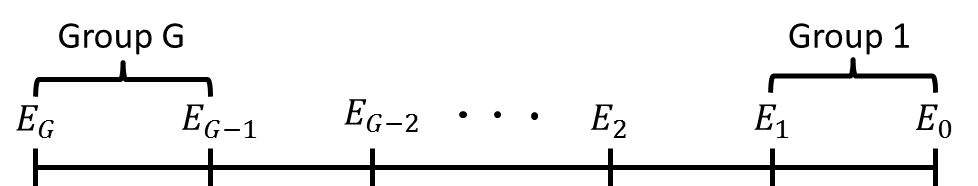
\includegraphics[width=0.8\textwidth]{MGillustration.png}
\end{center}

\end{frame}

%%%%%%%%%%%%%%%%%%%%%%%%%%%%%%%%%%%%%%%%%%%%%%%%%%%%%%%%%%%%%%%%%%%%%%%%%%%%%%%%

\begin{frame}[t]{Angle Discretization}

\begin{itemize}
    \item Select a set of azimuthal and polar angles $\alpha$ and $\mu$
\begin{align*}\scriptstyle
\bm\Omega &= \cos\left(\alpha\right)\sqrt{1-\mu^2}\bm i + \sin\left(\alpha\right)\sqrt{1-\mu^2}\bm j + \mu\bm k \\
\Rightarrow \bm\Omega_n &= \cos\left(\alpha_n\right)\sqrt{1-\mu_n^2}\bm i + \sin\left(\alpha_n\right)\sqrt{1-\mu_n^2}\bm j + \mu_n\bm k\ .
\end{align*}
\item A quadrature can be used with weights $w_n$ associated with each angle $\Omega_n$
\begin{subequations}
    \begin{equation*}\scriptstyle
    \intop d\Omega = \sum_{n=1}^N w_n = 4\pi\ ,
    \end{equation*}
    \begin{equation*}\scriptstyle
    \intop \bm\Omega d\Omega = \sum_{n=1}^N \bm\Omega_n w_n = 0\ ,
    \end{equation*}
    \begin{equation*}\scriptstyle
    \intop_{4\pi} f\left(\bm\Omega\right)d\Omega \approx \sum_{n=1}^N f_n w_n\ .
    \end{equation*}
\end{subequations}
\end{itemize}

\end{frame}

%%%%%%%%%%%%%%%%%%%%%%%%%%%%%%%%%%%%%%%%%%%%%%%%%%%%%%%%%%%%%%%%%%%%%%%%%%%%%%%%

\begin{frame}[t]{Transport-Corrected Scattering Approximation}

\begin{itemize}
\item Modifies self-scatter and total cross-sections to account for 
anisotropy while performing isotropic calculations
\item Neutron Leakage Conservation (NLC) Method: H-1
\begin{equation*}
\Sigma_{s0,g\rightarrow g} = \Sigma_{s0,g\rightarrow g} + \frac{1}{3D_g} 
- \Sigma_{t,g}
\end{equation*}
\item In-Scatter Method: B-11, C-12, O-16
\begin{equation*}
\Sigma_{s0,g\rightarrow g} = \Sigma_{s0,g\rightarrow g} - 
\frac{1}{\phi_{1,g}}\sum_{g'=1}^G \Sigma_{s1,g'\rightarrow g}\phi_{1,g'}
\end{equation*}
\item Out-Scatter Method: All other isotopes
\begin{equation*}
\Sigma_{s0,g\rightarrow g} = \Sigma_{s0,g\rightarrow g} - \sum_{g'=1}^G 
\Sigma_{s1,g\rightarrow g'}
\end{equation*}
\end{itemize}

\end{frame}

%%%%%%%%%%%%%%%%%%%%%%%%%%%%%%%%%%%%%%%%%%%%%%%%%%%%%%%%%%%%%%%%%%%%%%%%%%%%%%%%

\begin{frame}[t]{Collision Probabilities}

\begin{itemize}
    \item Used to calculate flux spectra in a pin cell
    \item Transport equation written so right-hand side is a single source term
    \begin{itemize}
        \item Assumes only scattering and fission sources
        \item Assumes isotropic scattering
    \end{itemize}
    \item For 1D, pin cell is discretized into $R$ rings, assuing flat source, flux, and cross section in each ring
    \item A matrix with elements $T_{g,r' \rightarrow r}$ can be determined
    \begin{itemize}
        \item Each element is probability of neutron born in group $g$ and region $r'$ reaching region $r$
        \item These probabilities are geometry-dependent, but have a general form for 1D cylindrical geometry
    \end{itemize}
    \item Flux in each ring can be calculated from matrix $\bm T$, sources $q$, and volumes $V$
\begin{equation*}\scriptstyle
\phi_{g,r} = \sum_{r'=1}^R T_{g,r'\rightarrow r} q_{g,r'} V_{r'}
\end{equation*}
\end{itemize}

\end{frame}

%%%%%%%%%%%%%%%%%%%%%%%%%%%%%%%%%%%%%%%%%%%%%%%%%%%%%%%%%%%%%%%%%%%%%%%%%%%%%%%%%

\begin{frame}
\begin{center}
\resizebox{0.5\textwidth}{!}{\begin{tikzpicture}[node distance=2cm]

% Start
\node (start) [startstop] {Start};

% CMFD
\node (homog) [process, right of=start, xshift=2.0cm] {Homogenize Cross-sections and Flux; Calculate $\tilde{D}$};
\node (iterCheck) [decision, below of=homog, yshift=-1.5cm] {First Iteration?};
\node (firstIter) [process, below of=iterCheck, xshift=-2.5cm, yshift=-1.0cm] {Set $\hat{D}=0$};
\node (laterIter) [process, below of=iterCheck, xshift=2.5cm, yshift=-1.0cm] {Calculate $\hat{D}$};
\node (matrix) [process, below of=firstIter, xshift=2.5cm] {Set up CMFD Matrix};
\node (3DCMFD) [process, below of=matrix] {3D CMFD Calculation};
\node (proj) [process, below of=3DCMFD] {Scale MOC flux with CMFD flux};

% Stop
\node (stop) [startstop, right of=proj, xshift=2.0cm] {Stop};

% Basic Arrows
\draw [arrow] (start) -- (homog);
\draw [arrow] (homog) -- (iterCheck);
\draw [arrow] (matrix) -- (3DCMFD);
\draw [arrow] (3DCMFD) -- (proj);
\draw [arrow] (proj) -- (stop);

% Fancy Arrows
\draw [arrow] (iterCheck) -| node[anchor=south] {yes} (firstIter);
\draw [arrow] (iterCheck) -| node[anchor=south] {no} (laterIter);
\draw [arrow] (firstIter) |- (matrix);
\draw [arrow] (laterIter) |- (matrix);

\end{tikzpicture}}
\end{center}
\end{frame}

%%%%%%%%%%%%%%%%%%%%%%%%%%%%%%%%%%%%%%%%%%%%%%%%%%%%%%%%%%%%%%%%%%%%%%%%%%%%%%%%%

\begin{frame}
\begin{center}
\resizebox{0.6\textwidth}{!}{\begin{tikzpicture}[node distance=2cm]

% Begin
\node (start) [startstop] {Start};

% Nodal
\node (radialTL) [process, right of=start, xshift=2.5cm] {Calculate radial transverse leakage source};
\node (sp3-0) [process, below of=radialTL] {Solve 0th moment equation};
\node (sp3-2) [process, below of=sp3-0] {Solve 2nd moment equation};
\node (convCheck) [decision, below of=sp3-2, yshift=-1.5cm] {Converged?};

% Stop
\node (stop) [startstop, right of=convCheck, xshift=2.5cm] {Stop};

% Basic Arrows
\draw [arrow] (start) -- (radialTL);
\draw [arrow] (radialTL) -- (sp3-0);
\draw [arrow] (sp3-0) -- (sp3-2);
\draw [arrow] (sp3-2) -- (convCheck);
\draw [arrow] (convCheck) -- node[anchor=north] {yes} (stop);

% Fancy Arrows
\draw [arrow] (convCheck) -| node[anchor=north] {no} ([xshift=-1.5cm]sp3-2.west) |- (sp3-0);

\end{tikzpicture}}
\end{center}
\end{frame}

%%%%%%%%%%%%%%%%%%%%%%%%%%%%%%%%%%%%%%%%%%%%%%%%%%%%%%%%%%%%%%%%%%%%%%%%%%%%%%%%%

\begin{frame}
\begin{center}
\resizebox{0.5\textwidth}{!}{\begin{tikzpicture}[node distance=2cm]

% Begin
\node (start) [startstop] {Start};
\node (init) [io, right of=start, xshift=2.5cm] {Input N$_{inners}$};

% MOC
\node (begin) [process, below of=init] {Set $n=0$};
\node (source) [process, below of=begin] {Calculate fission and axial transverse leakage sources};
\node (scatSource) [process, below of=source] {Calculate scattering source};
\node (MOC) [process, below of=scatSource] {2D MOC sweep over each energy group};
\node (MOCdone) [decision, below of=MOC, yshift=-1.5cm] {$n = N_{inners}$?};z
\node (stop) [startstop, right of=MOCdone, xshift=2.5cm] {Stop};

% Basic Arrows
\draw [arrow] (start) -- (init);
\draw [arrow] (init) -- (begin);
\draw [arrow] (begin) -- (source);
\draw [arrow] (source) -- (scatSource);
\draw [arrow] (scatSource) -- (MOC);
\draw [arrow] (MOC) -- (MOCdone);

% Fancy Arrows
\draw [arrow] (MOCdone) -| node[anchor=north] {no} ([xshift=-1.5cm]MOC.west) |- (scatSource);
\draw [arrow] (MOCdone) -- node[anchor=north] {yes} (stop);

\end{tikzpicture}}
\end{center}
\end{frame}

%%%%%%%%%%%%%%%%%%%%%%%%%%%%%%%%%%%%%%%%%%%%%%%%%%%%%%%%%%%%%%%%%%%%%%%%%%%%%%%%%

\begin{frame}
\vspace{-10pt}
\begin{center}
\resizebox{0.4\textwidth}{!}{\begin{tikzpicture}[node distance=2cm]

% Start
\node (start) [startstop] {Start};

% CMFD
\node (homog) [process, right of=start, xshift=2.0cm] {Homogenize cross-sections and flux; Calculate $\tilde{D}$};
\node (1dcpm) [process, below of=start, yshift=-0.5cm] {1D CP calculations};
\node (homogCP) [process, right of=1dcpm, xshift=2.0cm] {Re-homogenize cross-sections in partially rodded pin cells};
\node (iterCheck) [decision, below of=homogCP, yshift=-1.5cm] {First iteration?};
\node (firstIter) [process, below of=iterCheck, xshift=-2.5cm, yshift=-1.0cm] {Set $\hat{D}=0$};
\node (laterIter) [process, below of=iterCheck, xshift=2.5cm, yshift=-1.0cm] {Calculate $\hat{D}$};
\node (matrix) [process, below of=firstIter, xshift=2.5cm] {Set up CMFD matrix};
\node (3DCMFD) [process, below of=matrix] {3D CMFD calculation};
\node (proj) [process, below of=3DCMFD] {Scale MOC flux with CMFD flux};
\node (projCP) [process, below of=proj] {Homogenize partially rodded MOC cross-sections};

% Stop
\node (stop) [startstop, right of=projCP, xshift=2.0cm] {Stop};

% Basic Arrows
\draw [arrow] (start) -- (homog);
\draw [arrow] (1dcpm) -- (homogCP);
\draw [arrow] (homogCP) -- (iterCheck);
\draw [arrow] (matrix) -- (3DCMFD);
\draw [arrow] (3DCMFD) -- (proj);
\draw [arrow] (proj) -- (projCP);
\draw [arrow] (projCP) -- (stop);

% Fancy Arrows
\draw [arrow] (homog) |- ([yshift=-0.75cm]start.south) -| (1dcpm);
\draw [arrow] (iterCheck) -| node[anchor=south] {yes} (firstIter);
\draw [arrow] (iterCheck) -| node[anchor=south] {no} (laterIter);
\draw [arrow] (firstIter) |- (matrix);
\draw [arrow] (laterIter) |- (matrix);

\end{tikzpicture}}
\end{center}
\end{frame}

%%%%%%%%%%%%%%%%%%%%%%%%%%%%%%%%%%%%%%%%%%%%%%%%%%%%%%%%%%%%%%%%%%%%%%%%%%%%%%%%%

\begin{frame}[t]{2D/3D}

\begin{itemize}
    \item 2D MOC is used to generate homogenized cross sections
    \item MOC planes are homogenized onto Cartesian grid
    \item 3D S$_N$ is used to solve the 3D transport equation on the homogenized coarse mesh
\end{itemize}
\begin{center}
    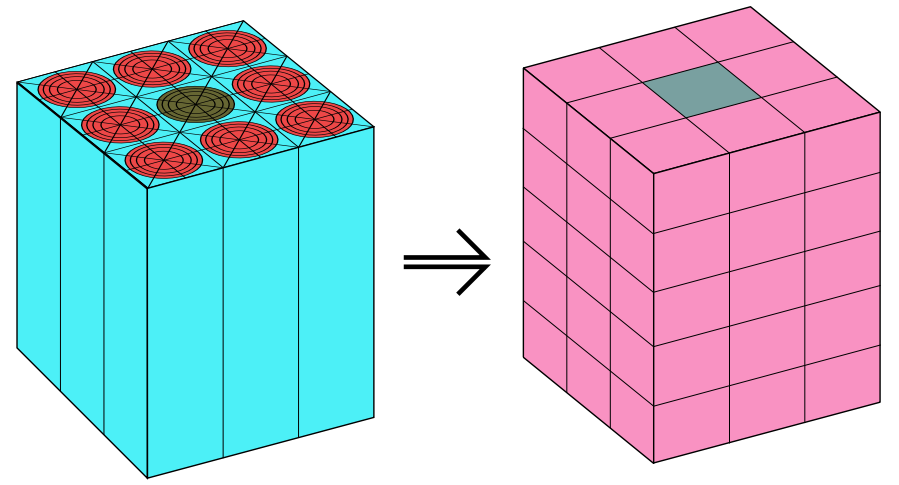
\includegraphics[width=0.7\textwidth]{2d-3d.png}
\end{center}

\end{frame}

%%%%%%%%%%%%%%%%%%%%%%%%%%%%%%%%%%%%%%%%%%%%%%%%%%%%%%%%%%%%%%%%%%%%%%%%%%%%%%%%

\begin{frame}[t]{1D MOC}

\begin{itemize}
    \item 1D MOC code developed that uses MOC cross sections and slab geometry
    \item Fixed source and eigenvalue calculations both supported
    \item Analysis of angular flux behavior for cross section mixtures could be performed
\end{itemize}
\begin{center}
    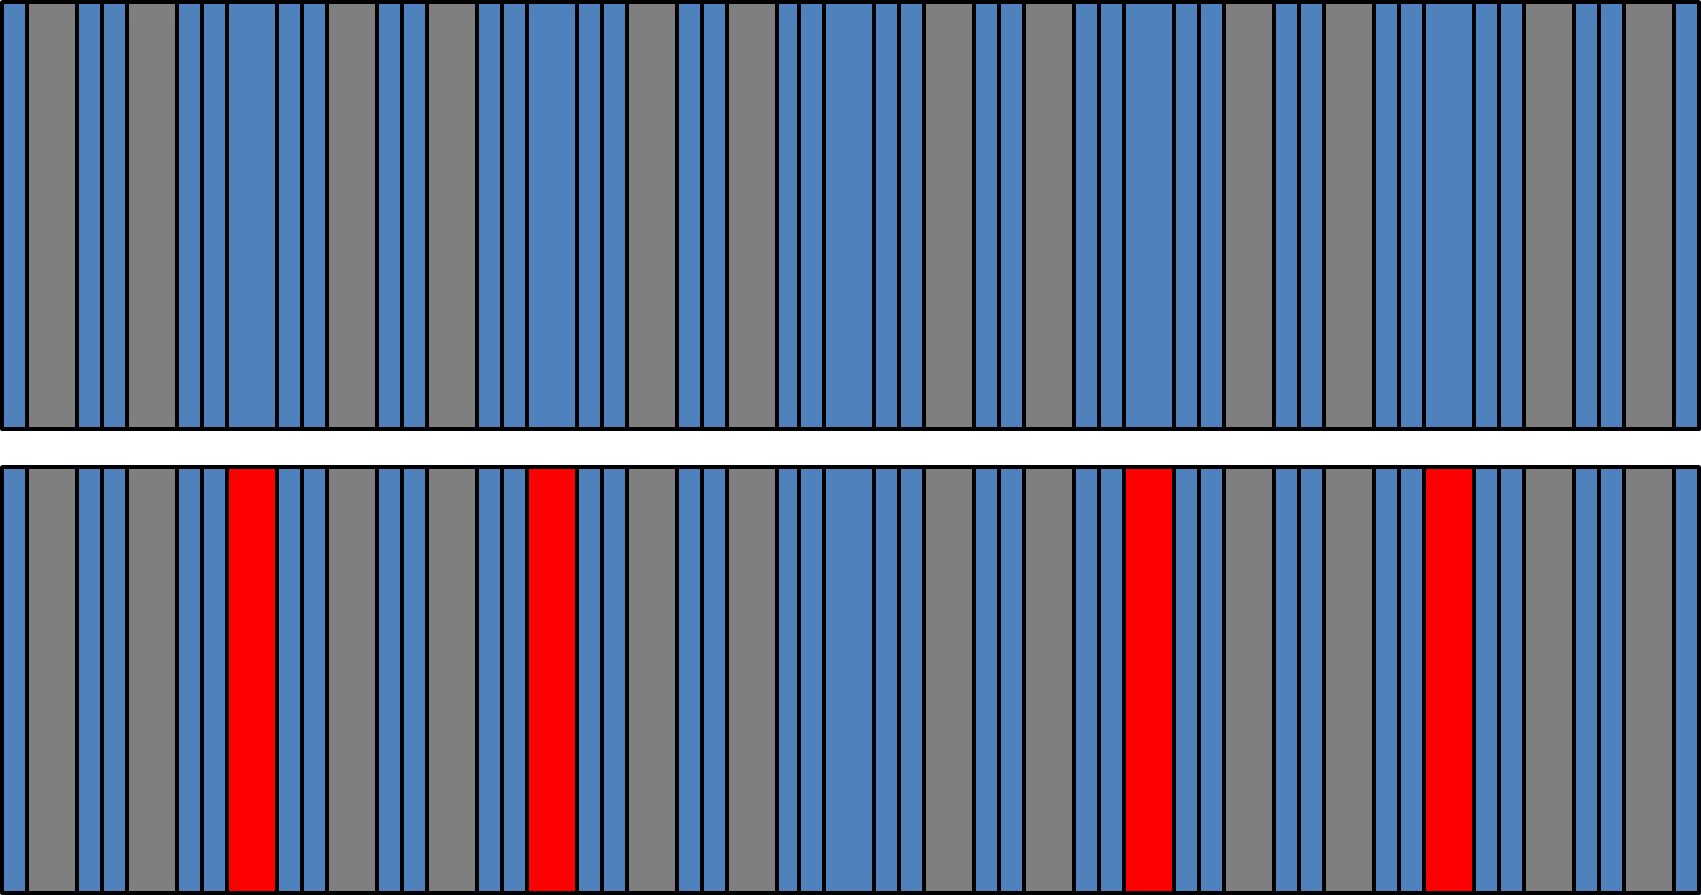
\includegraphics[width=0.6\textwidth]{1dmoc-3x17-geom.png}
\end{center}

\end{frame}

%%%%%%%%%%%%%%%%%%%%%%%%%%%%%%%%%%%%%%%%%%%%%%%%%%%%%%%%%%%%%%%%%%%%%%%%%%%%%%%%

\begin{frame}[t]{1D MOC -- Fixed Total Source}

\begin{itemize}
    \item Scalar flux, group 7
\end{itemize}
\begin{center}
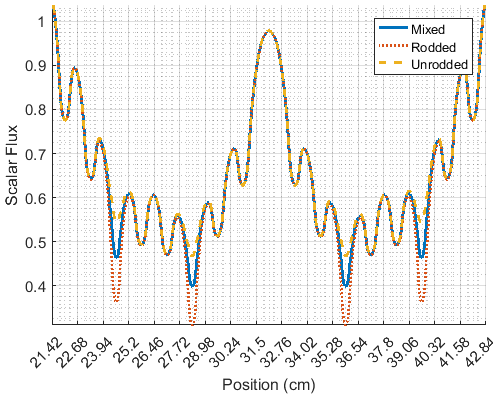
\includegraphics[width=0.5\textwidth]{1dmoc-50mix-fixedscat-scalflux7.png}
\end{center}

\end{frame}

%%%%%%%%%%%%%%%%%%%%%%%%%%%%%%%%%%%%%%%%%%%%%%%%%%%%%%%%%%%%%%%%%%%%%%%%%%%%%%%%

\begin{frame}[t]{1D MOC -- Fixed Total Source}

\begin{itemize}
    \item Rightgoing angular flux, group 1 (left) and 7 (right)
\end{itemize}

\begin{center}
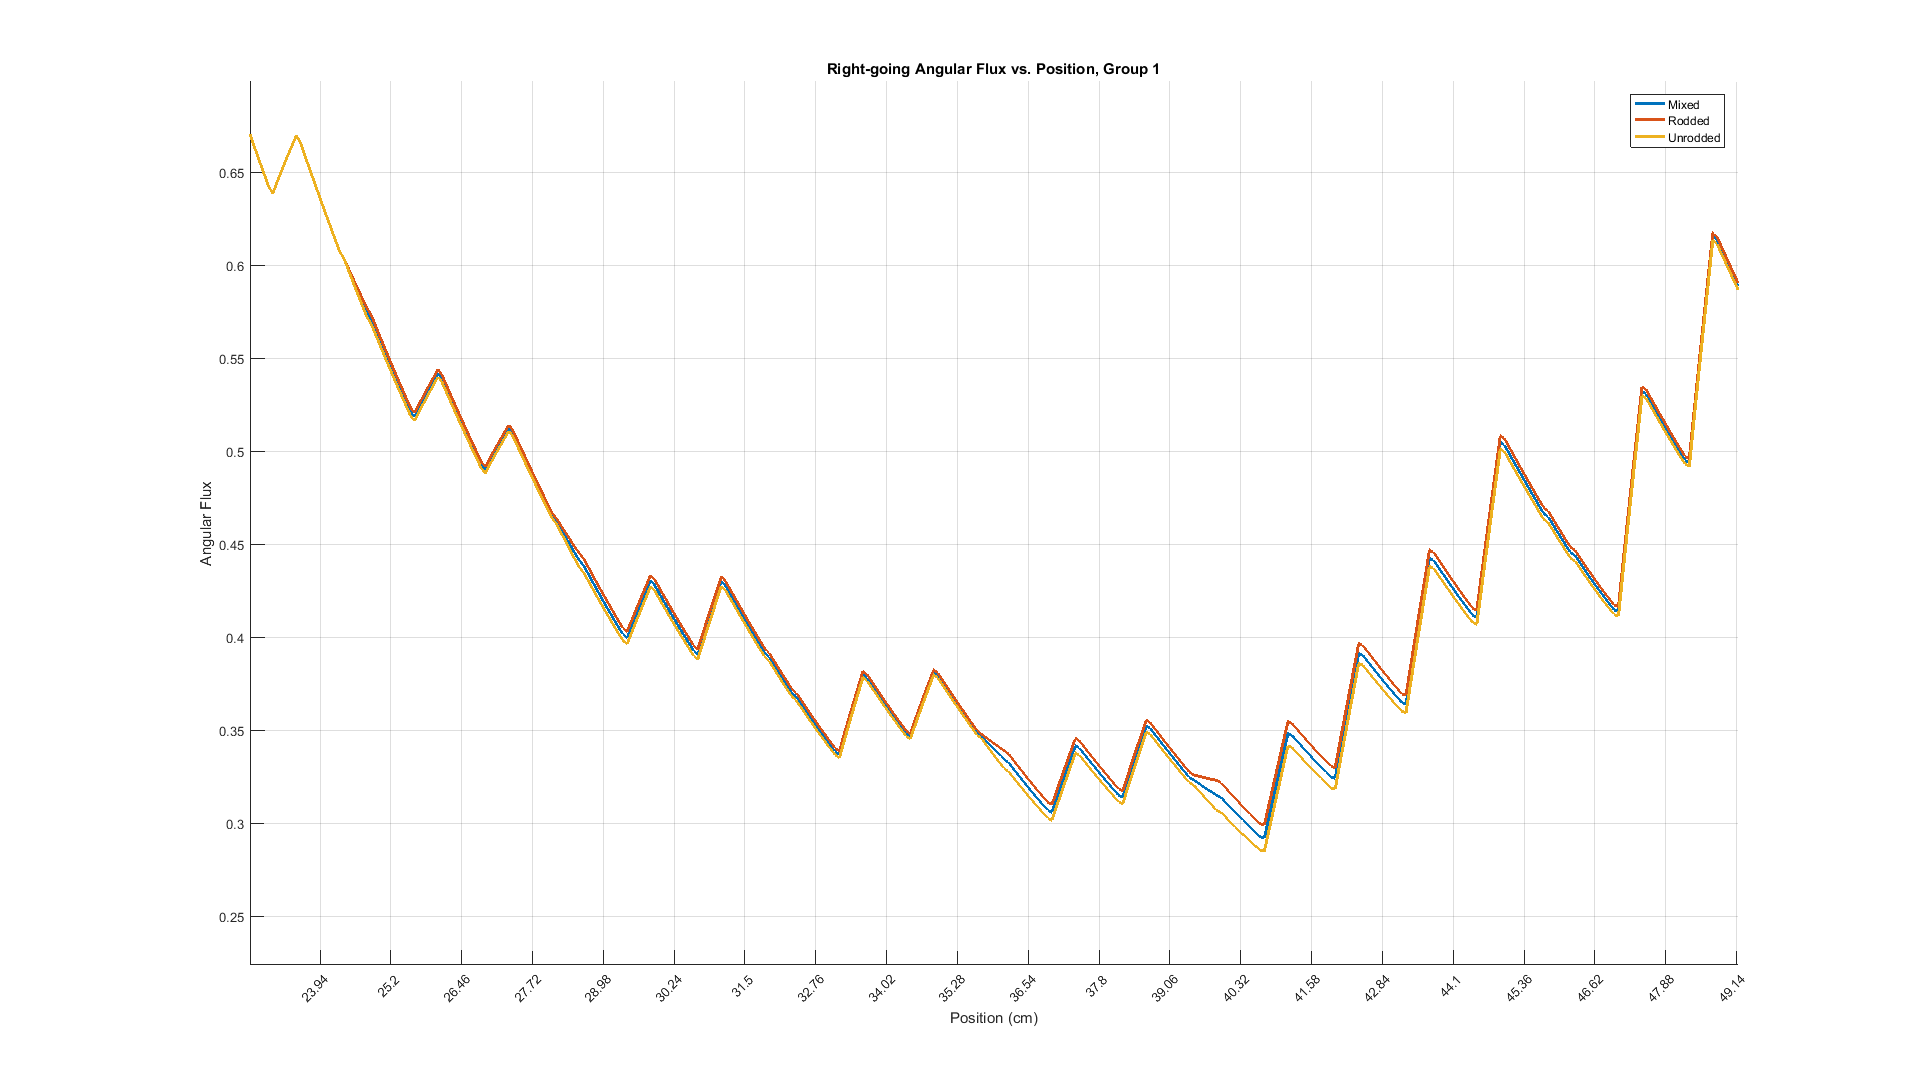
\includegraphics[width=0.45\textwidth]{1dmoc-50mix-fixedscat-angflux1.png} 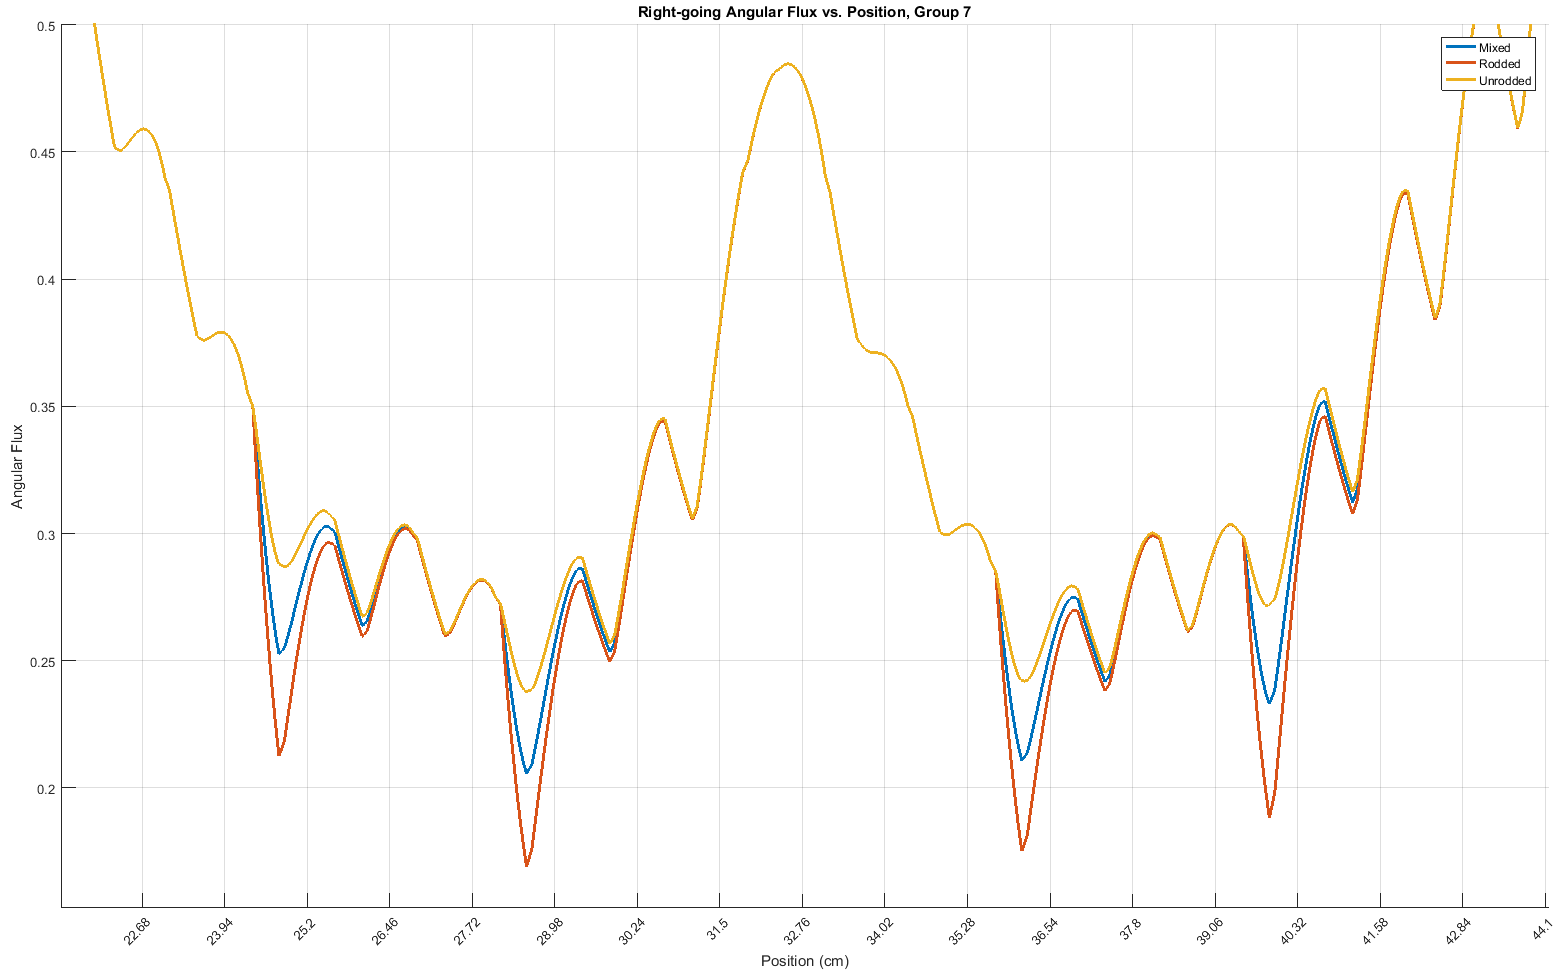
\includegraphics[width=0.45\textwidth]{1dmoc-50mix-fixedscat-angflux7.png}
\end{center}

\end{frame}

%%%%%%%%%%%%%%%%%%%%%%%%%%%%%%%%%%%%%%%%%%%%%%%%%%%%%%%%%%%%%%%%%%%%%%%%%%%%%%%%

\begin{frame}[t]{1D MOC -- Fixed Fission Source}

\begin{itemize}
    \item Rightgoing angular flux, group 1 (left) and 7 (right)
\end{itemize}
\begin{center}
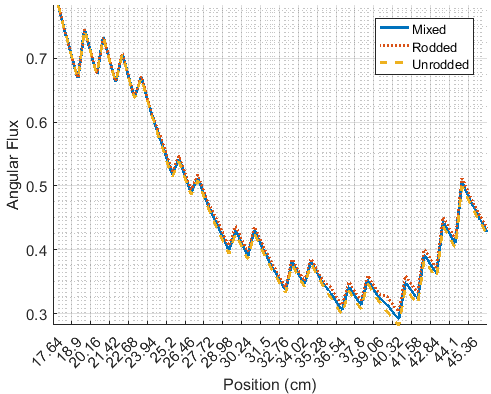
\includegraphics[width=0.45\textwidth]{1dmoc-50mix-angflux1.png} 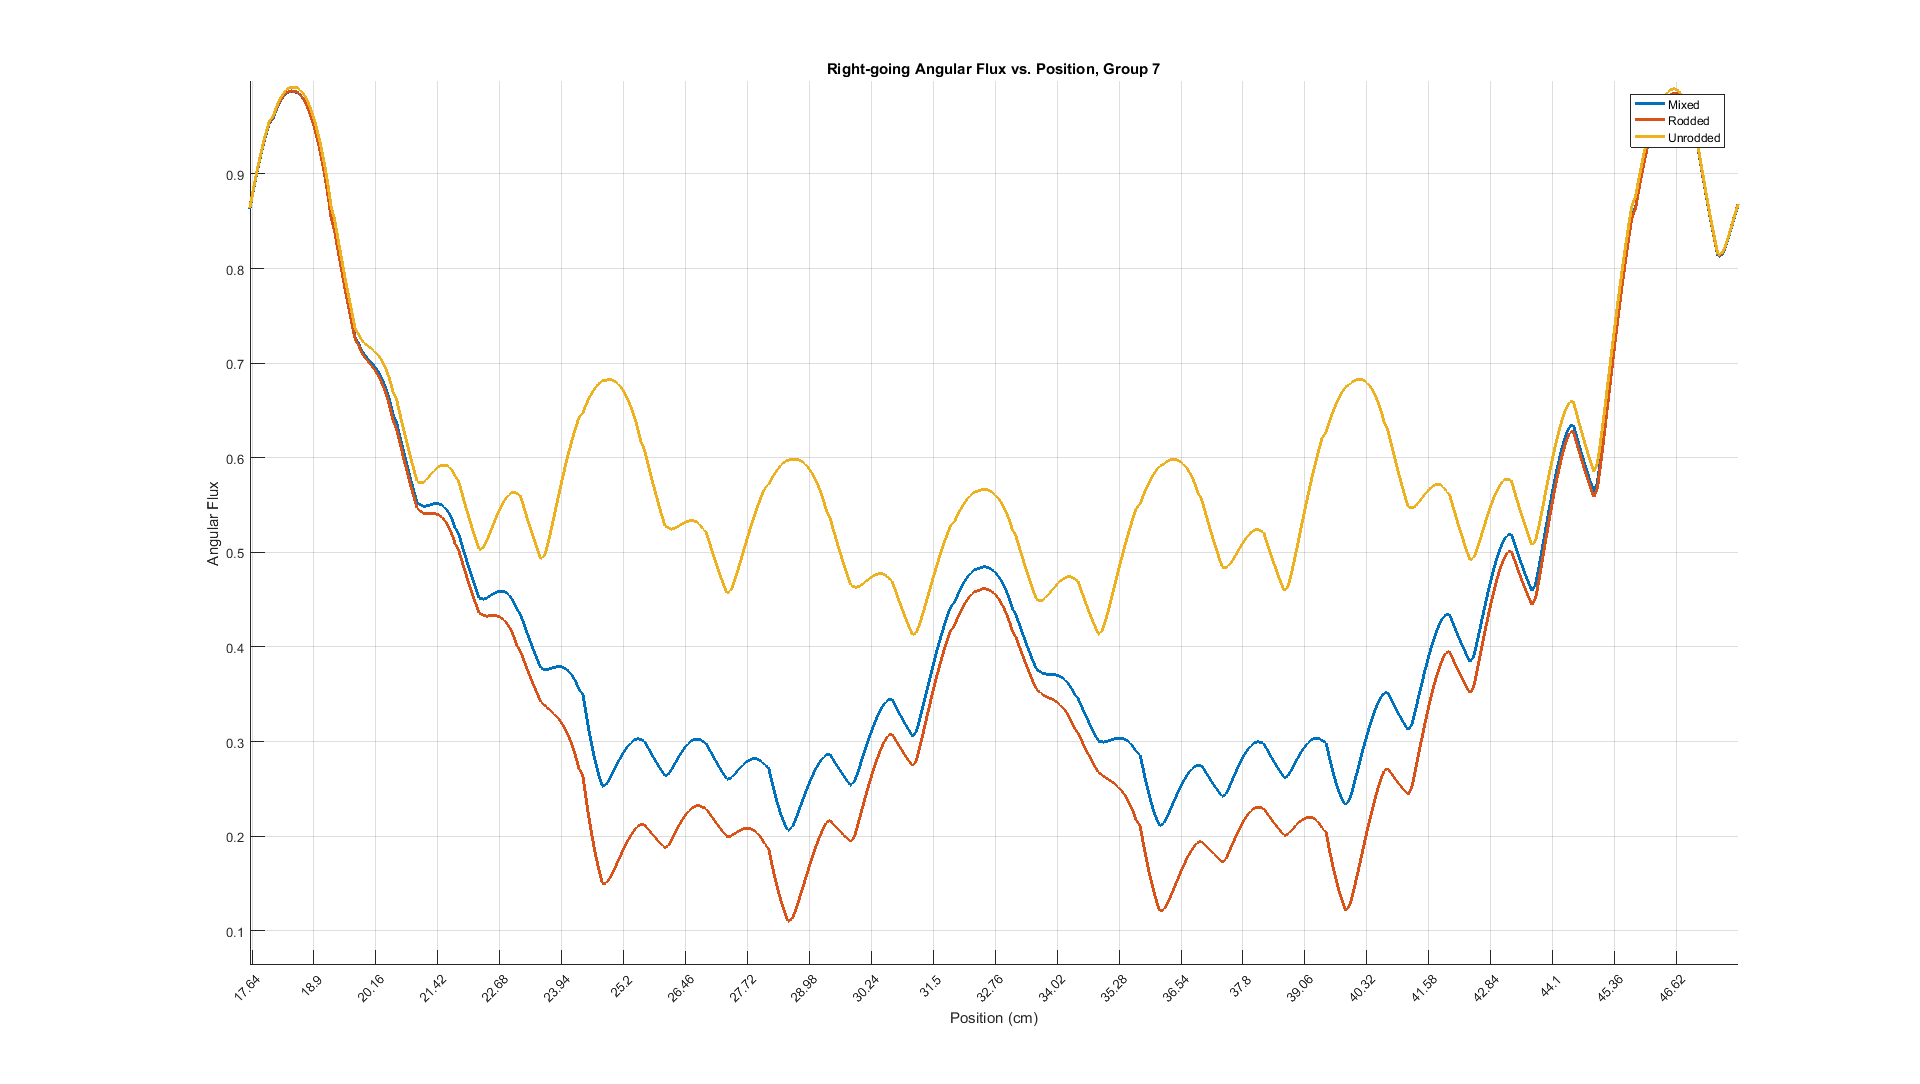
\includegraphics[width=0.45\textwidth]{1dmoc-50mix-angflux7.png}
\end{center}

\end{frame}

%%%%%%%%%%%%%%%%%%%%%%%%%%%%%%%%%%%%%%%%%%%%%%%%%%%%%%%%%%%%%%%%%%%%%%%%%%%%%%%%

\begin{frame}[t]{1D Subray MOC}

\begin{itemize}
    \item 1D MOC code developed that uses MOC cross sections and slab geometry
    \item Fixed source and eigenvalue calculations both supported
    \item Allowed for a prototype of subray MOC concept
\end{itemize}
\begin{center}
    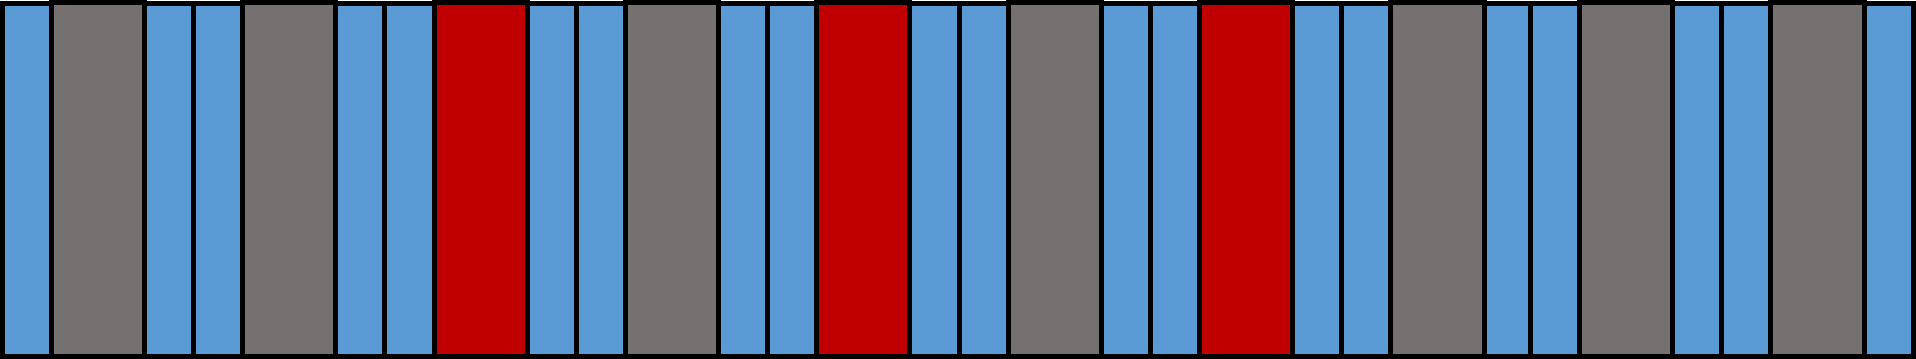
\includegraphics[width=0.8\textwidth]{10pin-slab-geometry.png}
\end{center}

\end{frame}

%%%%%%%%%%%%%%%%%%%%%%%%%%%%%%%%%%%%%%%%%%%%%%%%%%%%%%%%%%%%%%%%%%%%%%%%%%%%%%%%

\begin{frame}[t]{1D Subray MOC}

\begin{center}
    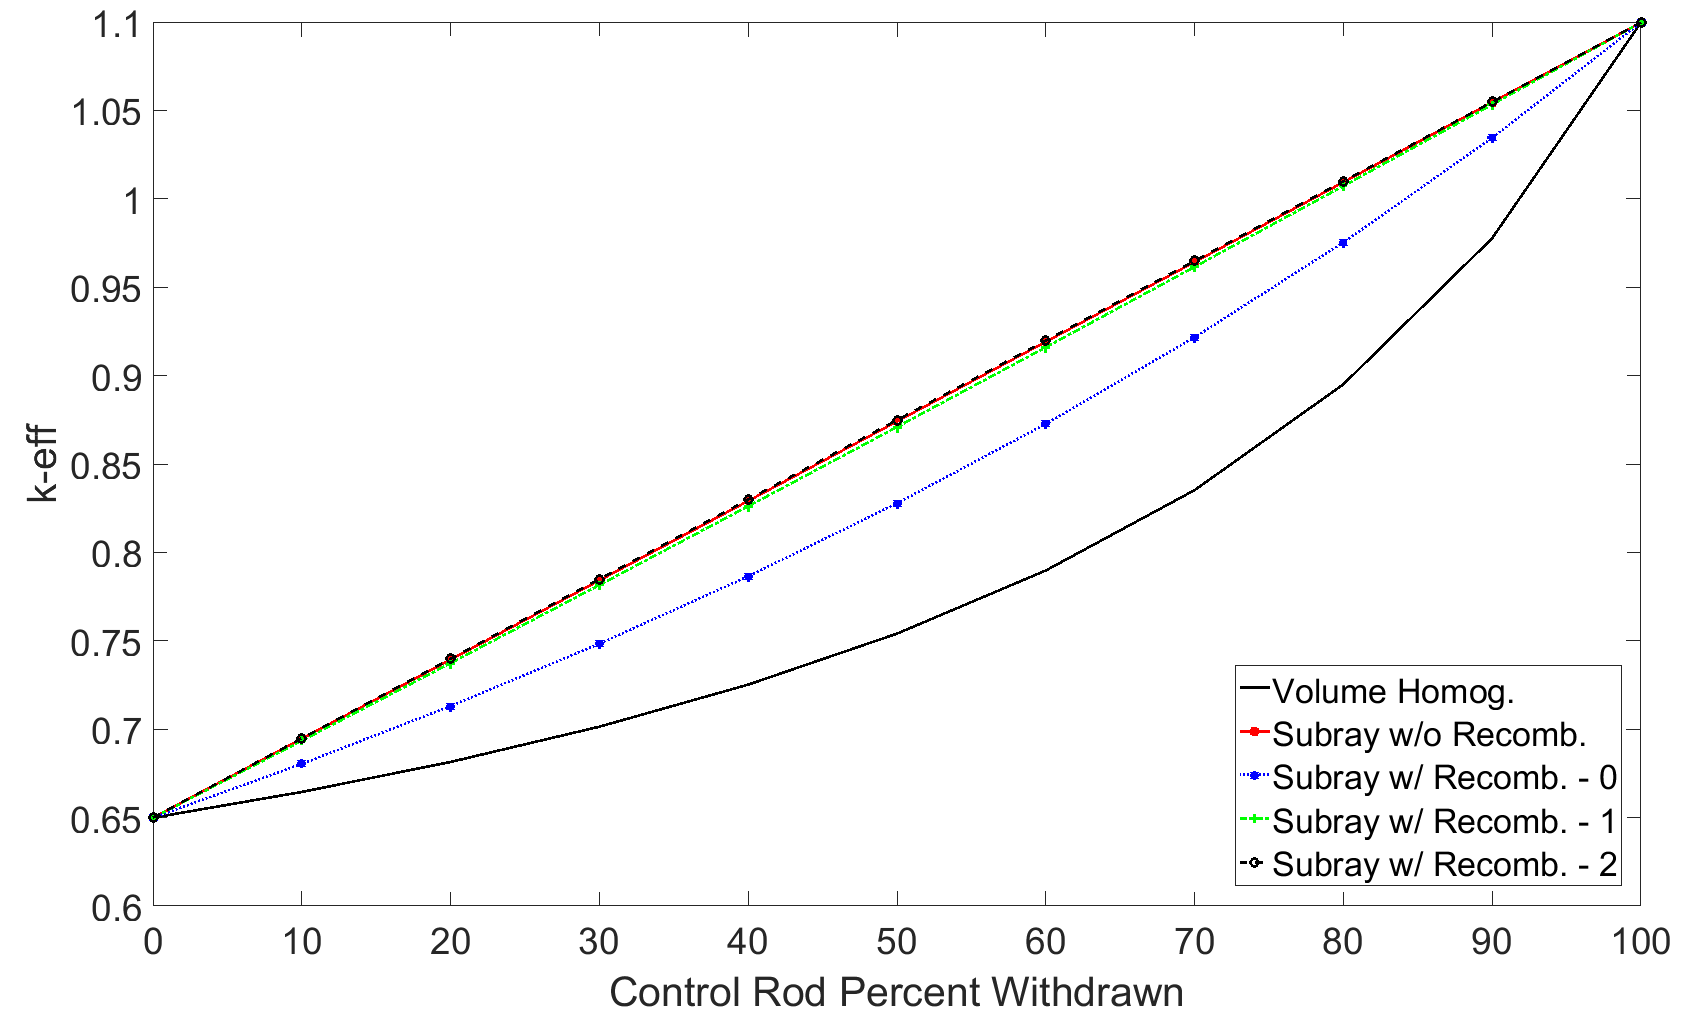
\includegraphics[width=0.8\textwidth]{keff_subray.png}
\end{center}

\end{frame}

%%%%%%%%%%%%%%%%%%%%%%%%%%%%%%%%%%%%%%%%%%%%%%%%%%%%%%%%%%%%%%%%%%%%%%%%%%%%%%%%

\begin{frame}[t]{1D Subray MOC}

\begin{itemize}
    \item 50\% rodded, scalar flux, group 1
\end{itemize}
\begin{center}
    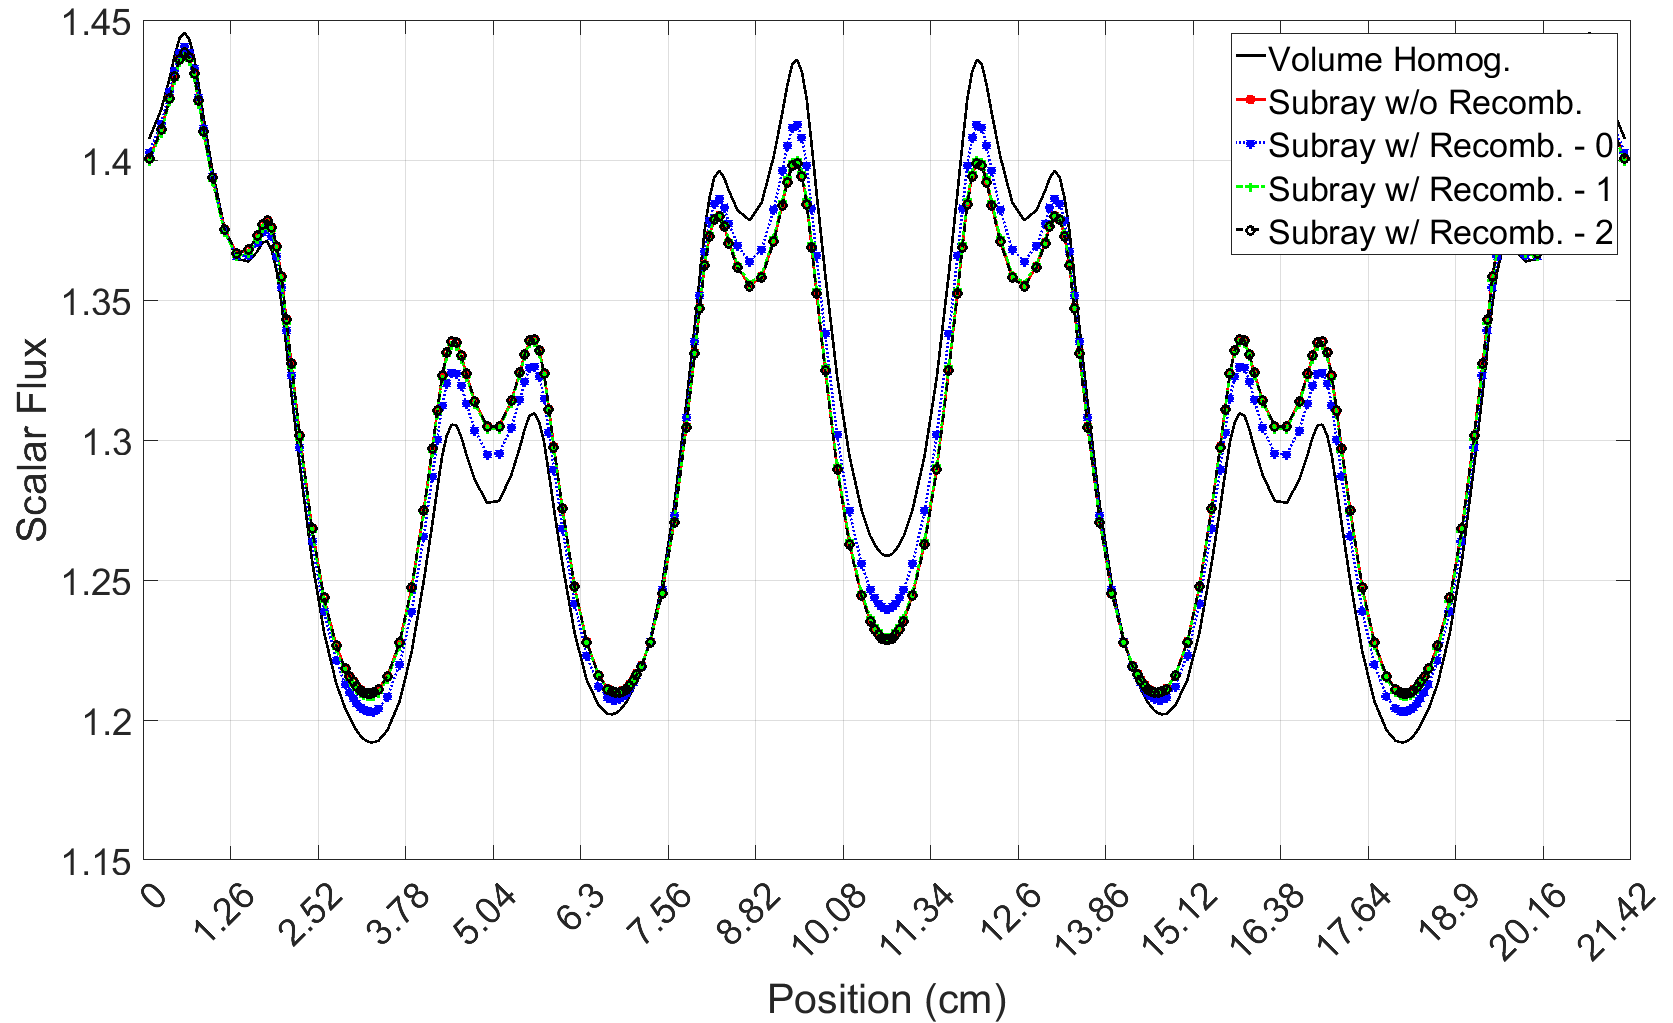
\includegraphics[width=0.8\textwidth]{scalflux1.png}
\end{center}

\end{frame}

%%%%%%%%%%%%%%%%%%%%%%%%%%%%%%%%%%%%%%%%%%%%%%%%%%%%%%%%%%%%%%%%%%%%%%%%%%%%%%%%

\begin{frame}[t]{1D Subray MOC}

\begin{itemize}
\item 50\% rodded, scalar flux, group 7
\end{itemize}
\begin{center}
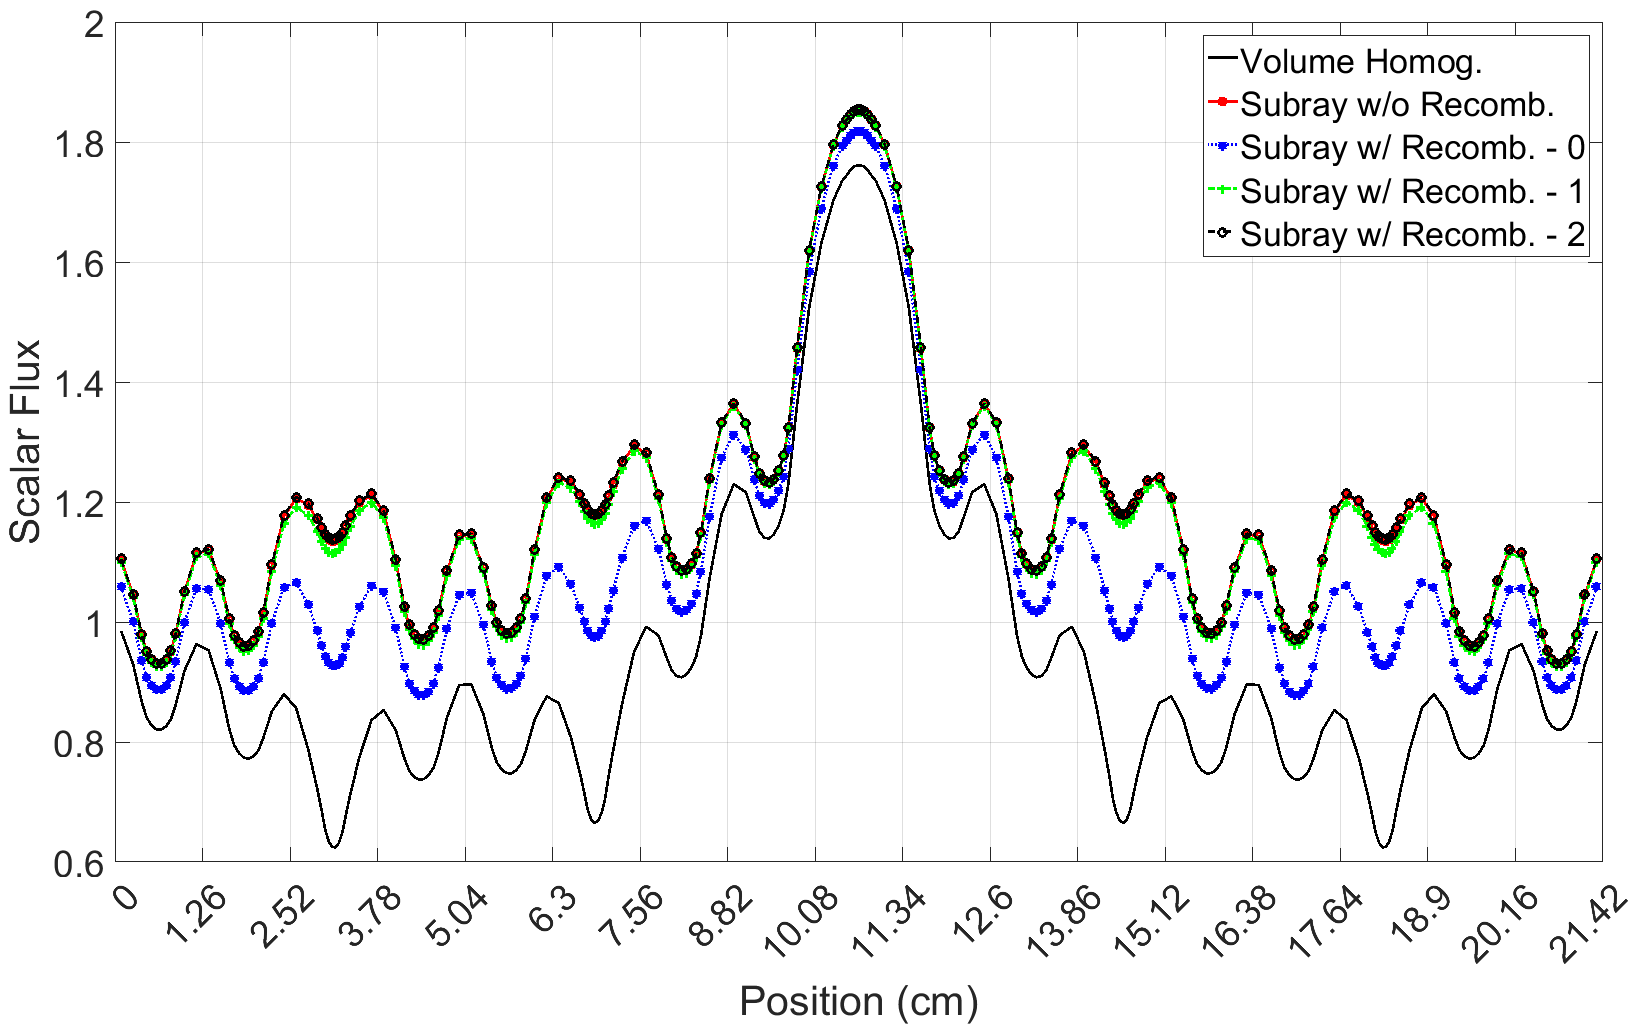
\includegraphics[width=0.8\textwidth]{scalflux7.png}
\end{center}

\end{frame}

\section*{References}
\renewcommand{\bibname}{References}
\bibliographystyle{../bibliography}
\bibliography{../bibliography}

\end{document}